\section{第4章\quad Smith圆图与阻抗匹配}
\begin{frame}
  Smith圆图是1939年由Phillip Smith在贝尔电话实验室工作时开发的,Smith圆图全面反映了反射系数与阻抗/导纳之间的相互换算关系,求解传输线问题是非常有用的。主要用在以下方面:
  \begin{itemize}
    \item 无耗传输线的分析
    \item 传输线的阻抗匹配
  \end{itemize}
\end{frame}

\subsection{Smith圆图}
\begin{frame}{Smith圆图的基本构成}
  上一章分析都是围绕如下公式及相互关系展开的:
  \begin{empheq}[box=\widefbox]{align*}
    Z_{in}(d)=\frac{V_L\cosh\gamma d+I_LZ_0\sinh\gamma d}{I_L\cosh\gamma d+\dfrac{V_L\sinh\gamma d}{Z_0}} & =Z_0\frac{Z_L+Z_0\tanh\gamma d}{Z_0+Z_L\tanh\gamma d}\\
    \text{无耗传输线:}& =Z_0\frac{Z_L+\mathrm{j}Z_0\tan\beta d}{Z_0+\mathrm{j}Z_L\tan\beta d}
  \end{empheq}
  \begin{columns}
    \begin{column}{0.45\linewidth}
      \begin{empheq}[box=\widefbox]{align*}
        \Gamma_L &=\frac{A_2}{A_1}=\frac{Z_L-Z_0}{Z_L+Z_0}\\
        &=\left\lvert\frac{Z_L-Z_0}{Z_L+Z_0}\right\rvert \mathrm{e}^{\mathrm{j}\phi_L}\\
        &=\lvert\Gamma_L\rvert \mathrm{e}^{\mathrm{j}\phi_L}
      \end{empheq}
    \end{column}
    \begin{column}{0.55\linewidth}
      \begin{empheq}[box=\widefbox]{align*}
        \rho=VSWR=\frac{\lvert V\rvert_{\mathrm{max}}}{\lvert V\rvert_{\mathrm{min}}}=\frac{1+\lvert\Gamma_L\rvert}{1-\lvert\Gamma_L\rvert}
      \end{empheq}
    \end{column}
  \end{columns}
\end{frame}

\begin{frame}{Smith圆图的基本构成}
  \begin{enumerate}
    \item 圆图概念
          \begin{itemize}
            \item 圆图是求解均匀传输线有关阻抗计算和阻抗匹配问题的一类曲线坐标图;
            \item 图上有两组坐标曲线:归一化阻抗或者导纳的实部和虚部的等值线簇,与反射系数的模和辐角的等值线簇;
            \item 所有这些等值线簇都是圆或圆弧(直线是圆的特例),故称为阻抗圆图或者导纳圆图,简称圆图。
          \end{itemize}
          \saveenum
  \end{enumerate}
  \begin{align*}
    z(d)=\frac{Z(d)}{Z_0}=\frac{1+\Gamma(d)}{1-\Gamma(d)}\quad\text{or}\quad\Gamma(d)=\frac{z(d)-1}{z(d)+1} \\
    z(d)=r(d)+\mathrm{j}x(d)=\lvert z\rvert \mathrm{e}^{\mathrm{j}\theta}                                   \\
    \Gamma(d)=\Gamma_{\mathrm{Re}}(d)+\mathrm{j}\Gamma_{\mathrm{Im}}(d)=\lvert\Gamma(d)\rvert \mathrm{e}^{\mathrm{j}\phi(d)}
  \end{align*}
\end{frame}

\begin{frame}{Smith圆图的基本构成}
  \begin{enumerate}
    \resume
    \item Smith圆图
          \begin{itemize}
            \item Smith圆图是通过双线性变换式,将$z$复平面上的$r=$常数和$x=$常数的二簇相互正交的直线分别变换成$\Gamma$复平面上的二簇相互正交的圆,并同$\Gamma$极坐标等值线簇$\lvert\Gamma\rvert=$常数和$\phi=$常数套印在一起而得到的圆图。
            \item 该图表是由\textbf{Phillip Smith}于1939年发明的,当时他在美国的RCA公司工作。Smith也许不是图表的第一位发明者,一位名叫Kurakawa的日本工程师声称早于其一年发明了这种图表。
          \end{itemize}
  \end{enumerate}
  \begin{align*}
    z(d)=\frac{Z(d)}{Z_0}=\frac{1+\Gamma(d)}{1-\Gamma(d)}\quad\text{or}\quad\Gamma(d)=\frac{z(d)-1}{z(d)+1} \\
    z(d)=r(d)+\mathrm{j}x(d)=\lvert z\rvert \mathrm{e}^{\mathrm{j}\theta}                                   \\
    \Gamma(d)=\Gamma_{\mathrm{Re}}(d)=\mathrm{j}\Gamma_{\mathrm{Im}}(d)=\lvert\Gamma(d)\rvert \mathrm{e}^{\mathrm{j}\phi(d)}
  \end{align*}
\end{frame}

\begin{frame}{Smith圆图的基本构成}
  \begin{itemize}
    \item 阻抗圆图\\
          阻抗圆图是由等反射系数圆和归一化等阻抗圆组成。
          \begin{enumerate}
            \item 等反射系数圆\\
                  距离终端$d$处的反射系数为
                  \begin{empheq}[box=\widefbox]{align*}
                    \Gamma(d)=\lvert\Gamma\rvert \mathrm{e}^{\mathrm{j}\phi(d)}=\lvert\Gamma_L\rvert \mathrm{e}^{\mathrm{j}(\phi_L-2\beta d)}=\Gamma_{\mathrm{Re}}+\mathrm{j}\Gamma_{\mathrm{Im}}
                  \end{empheq}
                  \saveenum
          \end{enumerate}
          表明,在复平面上等反射系数模$\lvert\Gamma\rvert$的轨迹是以坐标原点为圆心、$\lvert\Gamma_L\rvert$为半径的圆,这个圆称为等反射系数$\lvert\Gamma\rvert$圆。由于反射系数的模与驻波比是一一对应的,故又称为\textbf{等驻波比圆}。
  \end{itemize}
\end{frame}

\begin{frame}{Smith圆图的基本构成}
  线上移动的距离与转动角度之间的关系为
  \begin{columns}
    \begin{column}{0.4\linewidth}
      \begin{empheq}[box=\widefbox]{align*}
        \Gamma(d) &=\lvert\Gamma\rvert \mathrm{e}^{\mathrm{j}\phi}\\
        &=\lvert\Gamma_L\rvert \mathrm{e}^{\mathrm{j}(\phi_L-2\beta d)}\\
        \Delta\phi &=2\beta\Delta d\\
        &=\frac{4\pi}{\lambda}\Delta d
      \end{empheq}
      为了使用方便,有的圆图上标有两个方向的波长数数值,如图所示。向负载方向移动读里圈读数,向波源方向移动读外圈读数。
    \end{column}
    \begin{column}{0.6\linewidth}
      \begin{figure}
        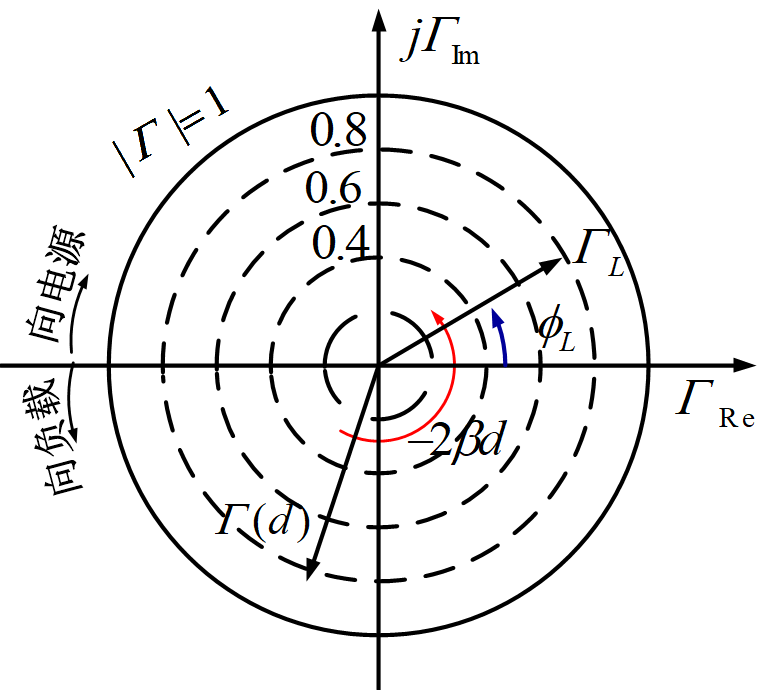
\includegraphics[width=6cm]{Cha4//reflect_coeff.png}
        \caption{反射系数圆}
      \end{figure}
    \end{column}
  \end{columns}
\end{frame}

\begin{frame}{Smith圆图的基本构成}
  \textbf{相角相等的反射系数的轨迹是单位圆内的径向线}
  \begin{columns}
    \begin{column}{0.4\linewidth}
      线上移动长度$\lambda/2$时,对应反射系数矢量转动一周。一般转动的角度用波长数(或电长度)$\Delta d/\lambda$表示,且标度波长数的零点位置通常选在$\phi=\pi$处。
    \end{column}
    \begin{column}{0.6\linewidth}
      \begin{figure}
        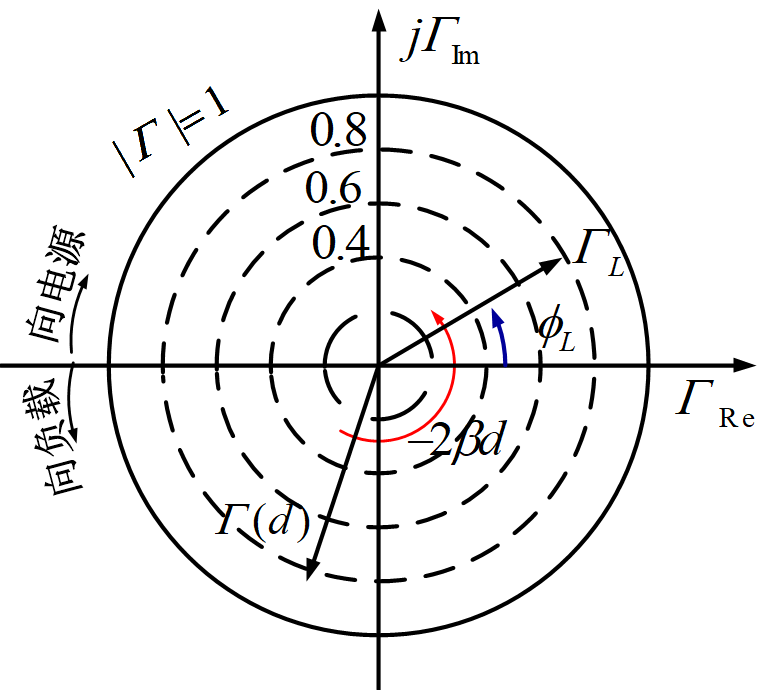
\includegraphics[width=5cm]{Cha4//reflect_coeff.png}
        \caption{等反射系数圆的波长数标度}
      \end{figure}
    \end{column}
  \end{columns}
  $\phi=0$\textbf{的径向线为各种不同负载阻抗情况下电压波腹点反射系数的轨迹;}\\
  $\phi=\pi$\textbf{的径向线为各种不同负载阻抗情况下电压波节点反射系数的轨迹。}
\end{frame}

\begin{frame}{Smith圆图的基本构成}
  \begin{itemize}
    \item 阻抗圆图
          \begin{enumerate}
            \resume
            \item 归一化阻抗圆
          \end{enumerate}
          \begin{empheq}[box=\widefbox]{align*}
            z_{in}(d)=\frac{Z_{in}(d)}{Z_0}=\frac{1+\Gamma(d)}{1-\Gamma(d)}
          \end{empheq}
  \end{itemize}
  \begin{align*}
    z_{in}(d) & =\frac{1+(\Gamma_{\mathrm{Re}}+\mathrm{j}\Gamma_{\mathrm{Im}})}{1-(\Gamma_{\mathrm{Re}}+\mathrm{j}\Gamma_{\mathrm{Im}})}                                                                                                     \\
              & =\frac{1-(\Gamma^{2}_{\mathrm{Re}}+\Gamma^{2}_{\mathrm{Im}})}{(1-\Gamma_{\mathrm{Re}})^2+\Gamma_{\mathrm{Im}}^{2}}+\mathrm{j}\frac{2\Gamma_{\mathrm{Im}}}{(1-\Gamma_{\mathrm{Re}})^2+\Gamma_{\mathrm{Im}}^{2}}=r+\mathrm{j}x
  \end{align*}
  \begin{empheq}[box=\widefbox]{align*}
    \left(\Gamma_{\mathrm{Re}}-\frac{r}{r+1}\right)^2+\Gamma_{\mathrm{Im}}^{2}=\frac{1}{(r+1)^2}\quad \text{归一化电阻轨迹方程}\\
    (\Gamma_{\mathrm{Re}}-1)^2+\left(\Gamma_{\mathrm{Im}}-\frac{1}{x}\right)^2=\left(\frac{1}{x}\right)^2\quad \text{归一化电抗轨迹方程}
  \end{empheq}
  \footnotesize{特征参数,是形成统一Smith圆图的最关键点,它包含了阻抗归一和电长度归一。}
\end{frame}

\begin{frame}{Smith圆图的基本构成}
  \only<1>{\begin{columns}
      \begin{column}{0.55\linewidth}
        \begin{empheq}[box=\widefbox]{align*}
          (\Gamma_{\mathrm{Re}}-1)^2+\left(\Gamma_{\mathrm{Im}}-\frac{1}{x}\right)^2=\left(\frac{1}{x}\right)^2
        \end{empheq}
      \end{column}
      \begin{column}{0.45\linewidth}
        \begin{figure}
          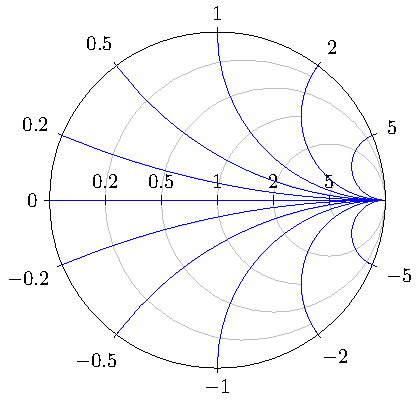
\includegraphics[width=5cm]{Cha4//fig4-4.pdf}
          \caption{归一化电抗圆}
        \end{figure}
      \end{column}
    \end{columns}}
  \only<2>{\begin{columns}
      \begin{column}{0.45\linewidth}
        \begin{figure}
          \includegraphics[width=5cm]{Cha4//fig4-3.pdf}
          \caption{归一化电阻圆}
        \end{figure}
      \end{column}
      \begin{column}{0.55\linewidth}
        \begin{empheq}[box=\widefbox]{align*}
          \left(\Gamma_{\mathrm{Re}}-\frac{r}{r+1}\right)^2+\Gamma_{\mathrm{Im}}^2=\frac{1}{(r+1)^2}
        \end{empheq}
      \end{column}
    \end{columns}}
\end{frame}

\begin{frame}{Smith圆图的基本构成}
  电阻圆始终和直线$\Gamma_r=1$相切
  \begin{columns}
    \begin{column}{0.42\linewidth}
      \begin{figure}
        \includegraphics[width=4.55cm]{Cha4//fig4-3.pdf}
        \caption{归一化电阻圆}
      \end{figure}
    \end{column}

    \begin{column}{0.58\linewidth}
      \begin{table}
        \caption{电阻圆圆心位置及半径}
        \begin{tabular}{|c|c|c|c|}
          \hline
          \multirow{2}*{$r$}                       &
          \multicolumn{2}{c|}{\footnotesize{圆心坐标}} &
          \multirow{2}*{\footnotesize{半径} $\left(\frac{1}{1+r}\right)$}                            \\ \cline{2-3}
                                                   & $\Gamma_r=\frac{r}{1+r}$ & $\Gamma_i=0$ &     \\ \hline
          0                                        & 0                        & 0            & 1   \\ \hline
          1                                        & 1/2                      & 0            & 1/2 \\ \hline
          2                                        & 2/3                      & 0            & 1/3 \\ \hline
        \end{tabular}
        %\label{table1}
      \end{table}
    \end{column}
  \end{columns}
  \begin{empheq}[box=\widefbox]{align*}
    \left(\Gamma_{\mathrm{Re}}-\frac{r}{r+1}\right)^2+\Gamma_{\mathrm{Im}}^2=\frac{1}{(r+1)^2}
  \end{empheq}
\end{frame}

\begin{frame}{Smith圆图的基本构成}
  电抗圆圆心坐标和半径
  \begin{empheq}[box=\widefbox]{align*}
    (\Gamma_{\mathrm{Re}}-1)^2+\left(\Gamma_{\mathrm{Im}}-\frac{1}{x}\right)^2=\left(\frac{1}{x}\right)^2
  \end{empheq}
  \begin{columns}
    \begin{column}{0.58\linewidth}
      \begin{table}
        \caption{电抗圆圆心位置及半径}
        \begin{tabular}{|c|c|c|c|}
          \hline
          \multirow{2}*{$x$}                       &
          \multicolumn{2}{c|}{\footnotesize{圆心坐标}} &
          \multirow{2}*{\footnotesize{半径} $\left(\frac{1}{x}\right)$}                               \\ \cline{2-3}
                                                   & $\Gamma_r=1$ & $\Gamma_i=\frac{1}{x}$ &        \\ \hline
          0                                        & 1            & \infty                 & \infty \\ \hline
          \pm0.5                                   & 1            & \pm2                   & 2      \\ \hline
          \pm1                                     & 1            & \pm1                   & 1      \\ \hline
        \end{tabular}
      \end{table}
    \end{column}

    \begin{column}{0.42\linewidth}
      \begin{figure}
        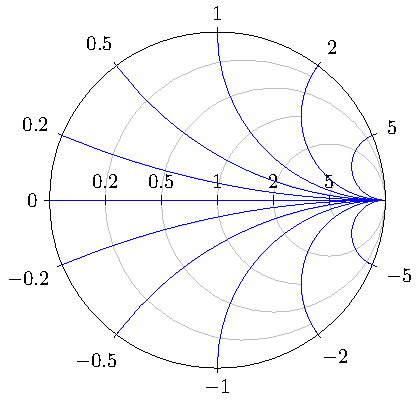
\includegraphics[width=4.55cm]{Cha4//fig4-4.pdf}
        \caption{归一化电抗圆}
      \end{figure}
    \end{column}
  \end{columns}
\end{frame}

\begin{frame}{Smith圆图的基本构成}
  将等电阻圆和等电抗圆绘制在同一张图上,得到阻抗圆图。
  \centering
  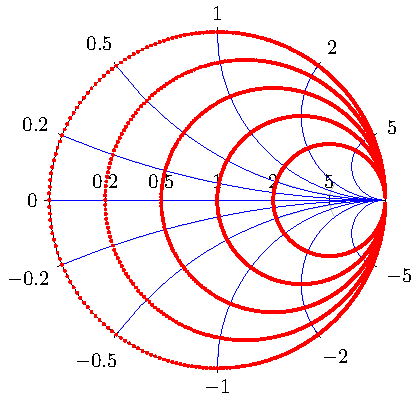
\includegraphics[width=8cm]{Cha4//fig4-5.pdf}
\end{frame}

\begin{frame}{Smith圆图的特点}
  \begin{columns}
    \begin{column}{0.4\linewidth}
      \textbf{阻抗圆图有如下几个特点}
      \begin{itemize}
        \item 圆图上有三个特殊点:
              \footnotesize{\textbf{匹配点}(O点)\\
                其坐标为(0,0)\\
                $r=1,x=0$ \\
                $\lvert\Gamma\rvert=0,\rho=1$\\
                \textbf{短路点}(C点)\\
                其坐标为(-1,0)\\
                $r=0,x=0,\lvert\Gamma\rvert=1$ \\
                $\rho=\infty,\phi=\pi$ \\
                \textbf{开路点}(D点)\\
                其坐标为(1,0)\\
                $r=\infty,x=\infty,\lvert\Gamma\rvert=1$ \\
                $\rho=\infty,\phi=0$}
      \end{itemize}

    \end{column}
    \begin{column}{0.6\linewidth}
      \only<1>{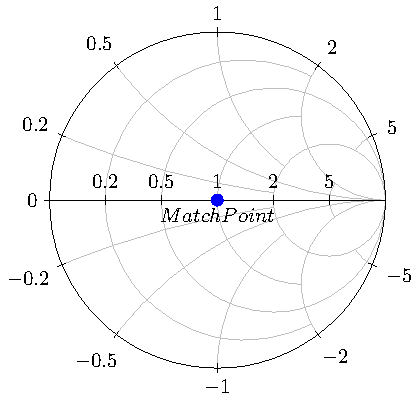
\includegraphics[width=7cm]{Cha4//MatchShortOpen1.pdf}}
      \only<2>{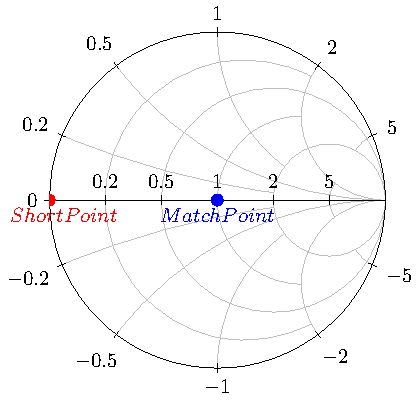
\includegraphics[width=7cm]{Cha4//MatchShortOpen2.pdf}}
      \only<3>{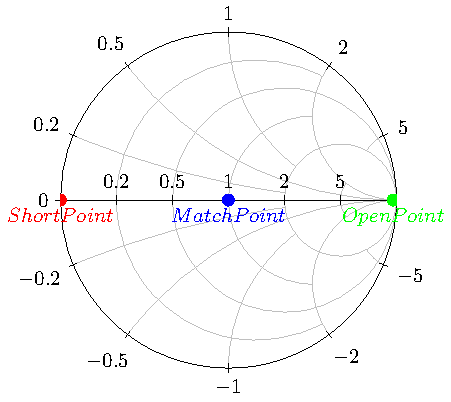
\includegraphics[width=7cm]{Cha4//MatchShortOpen3.pdf}}
    \end{column}
  \end{columns}
\end{frame}

\begin{frame}{Smith圆图的特点}
  \begin{columns}
    \begin{column}{0.4\linewidth}
      \begin{itemize}
        \item 圆图上有三条特殊线:
              \footnotesize{圆图上实轴为$x=0$的轨迹,\\
                \textbf{正半实轴}为电压波腹点的轨迹,线上$R$值为驻波比读数。\\
                \textbf{负半实轴}为电压波节点的轨迹,线上的$R$值为行波系数$K$的读数。\\
                \textbf{最外面的单位圆}为$R=0$的纯电抗轨迹,即为$\lvert\Gamma\rvert=1$的全反射系数圆的轨迹.\\}
        \item 圆上有两个特殊面
              \footnotesize{圆图实轴以上的上半平面是\textbf{感性}阻抗的轨迹;实轴以下的下半平面是\textbf{容性}阻抗的轨迹。}
      \end{itemize}
    \end{column}
    \begin{column}{0.6\linewidth}
      \only<1>{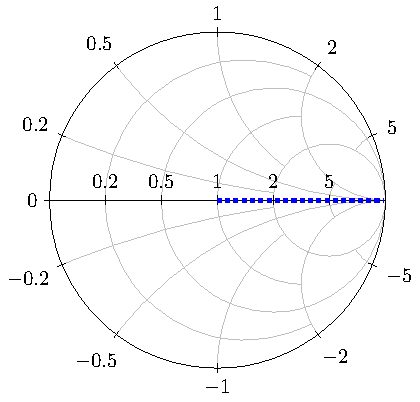
\includegraphics[width=7cm]{Cha4//bofubojie1.pdf}}
      \only<2>{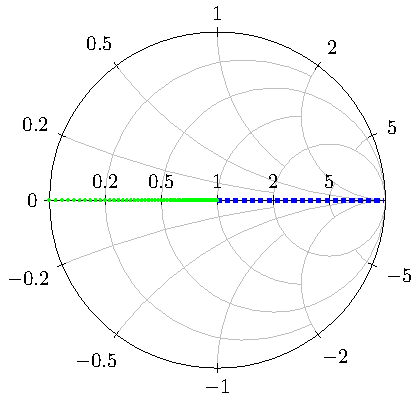
\includegraphics[width=7cm]{Cha4//bofubojie2.pdf}}
      \only<3>{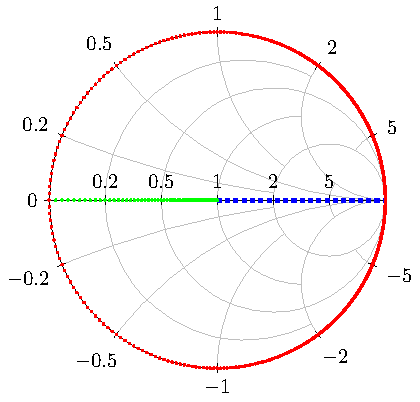
\includegraphics[width=7cm]{Cha4//bofubojie3.pdf}}
    \end{column}
  \end{columns}
\end{frame}

\begin{frame}{Smith圆图的特点}
  \begin{columns}
    \begin{column}{0.4\linewidth}
      \begin{itemize}
        \item \footnotesize{圆图上有两个旋转方向,在传输线上向负载方向移动时,则在圆图上沿等反射系数圆逆时针方向旋转;反之,在传输线上向波源方向移动时,
                则在圆图上沿等反射系数圆顺时针方向旋转。}
        \item \footnotesize{圆图上任意一点对应四个参量:$x$,$r$,$\lvert\Gamma\rvert$和$\phi$,知道前两个参量或后两个参量
                均可确定该点在圆图上的位置。}
        \item \footnotesize{若传输线上某一位置对应于圆图上的A点,则A点的读数即为该位置的输入阻抗归一化值$r=\mathrm{j}x$;若关
                于O点的A点对称点为B点,则B点的读数即为该位置的输入导纳归一化值$g+\mathrm{j}b$。}
      \end{itemize}
    \end{column}

    \begin{column}{0.6\linewidth}
      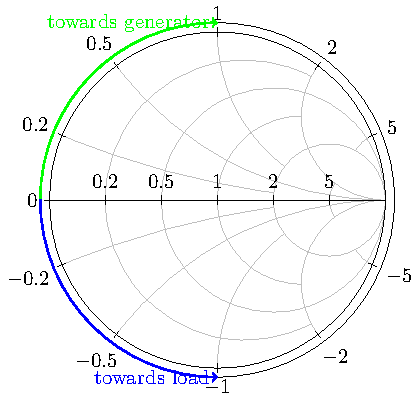
\includegraphics[width=7cm]{Cha4//xuanxiang.pdf}
    \end{column}

  \end{columns}
\end{frame}

\begin{frame}{Smith圆图的特点}
  \textbf{使用圆图应注意以下特点}\\
  \begin{columns}
    \begin{column}{0.4\linewidth}
      \begin{itemize}
        \item \footnotesize{当圆图作为阻抗圆图时,相角为0的反射系数位于OD上,相角增大,反射系数矢量沿逆时针方向转动;当圆图作为
                导纳圆图时,相角为0的反射系数位于OC上,相角增大,反射系数矢量仍沿逆时针方向转动。}
        \item \footnotesize{与阻抗圆图相反,作为导纳圆图使用时,D点为短路点,C点为开路点,线段OD为电压波节点归一化阻抗的轨迹,线
                段OC为电压波腹点归一化阻抗的轨迹}
        \item \footnotesize{$z(d)$与$y(d)$在同一反射系数圆上,相应位置差$180^{\circ}$}
      \end{itemize}
    \end{column}
    \begin{column}{0.6\linewidth}
      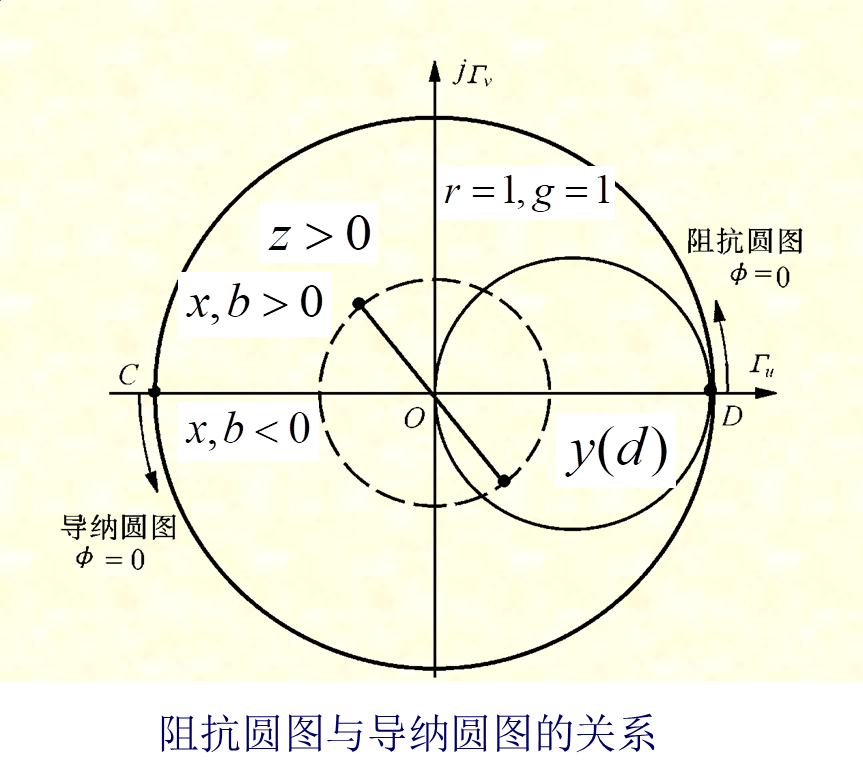
\includegraphics[width=7cm]{Cha4//Z_Yyuantu.png}
    \end{column}
  \end{columns}
\end{frame}

\begin{frame}{Smith圆图的应用}
  Smith圆图的基本功能
  \begin{center}
    \begin{tabular}{|c|c|}
      \hline
      1 & 已知阻抗$Z$,求导纳$Y$(或逆问题)                  \\
      \hline
      2 & 已知阻抗$Z$,求反射系数$\Gamma$和$\rho$(或逆问题)    \\
      \hline
      3 & 已知阻抗$Z$和$\phi$求输入阻抗$Z_{in}$(或逆问题)     \\
      \hline
      4 & 已知驻波比和最小点$d_{\mathrm{min}}$,求$Z_{in}$ \\
      \hline
    \end{tabular}
  \end{center}
\end{frame}

\begin{frame}{Smith圆图的应用}
  例1 \quad 特性阻抗$Z_0=50\Omega$,负载阻抗$Z_L=100+j50\Omega$,求距负载$0.24\lambda$处输入阻抗。\\
  解:归一化负载阻抗$z_L=2+\mathrm{j}1$\\
  \begin{columns}
    \begin{column}{0.4\linewidth}
      1)\quad 向电源方向旋转$0.213\lambda$
      \begin{flalign*}
        \phi=\arctan(1/2)                         &  & \\
        \frac{2\pi}{\lambda/2}=\frac{\pi-\phi}{l} &  & \\
        l =(\pi-0.4636)\lambda/4\pi               &  & \\
        =0.213\lambda                             &  &
      \end{flalign*}
      2)\quad 旋转$0.24\lambda$到$z_{in}$
      \begin{align*}
        z_{in}=0.42-j0.25\rightarrow\times 50 \\
        \rightarrow 21-j12.5\Omega
      \end{align*}
    \end{column}
    \begin{column}{0.6\linewidth}

      \only<1>{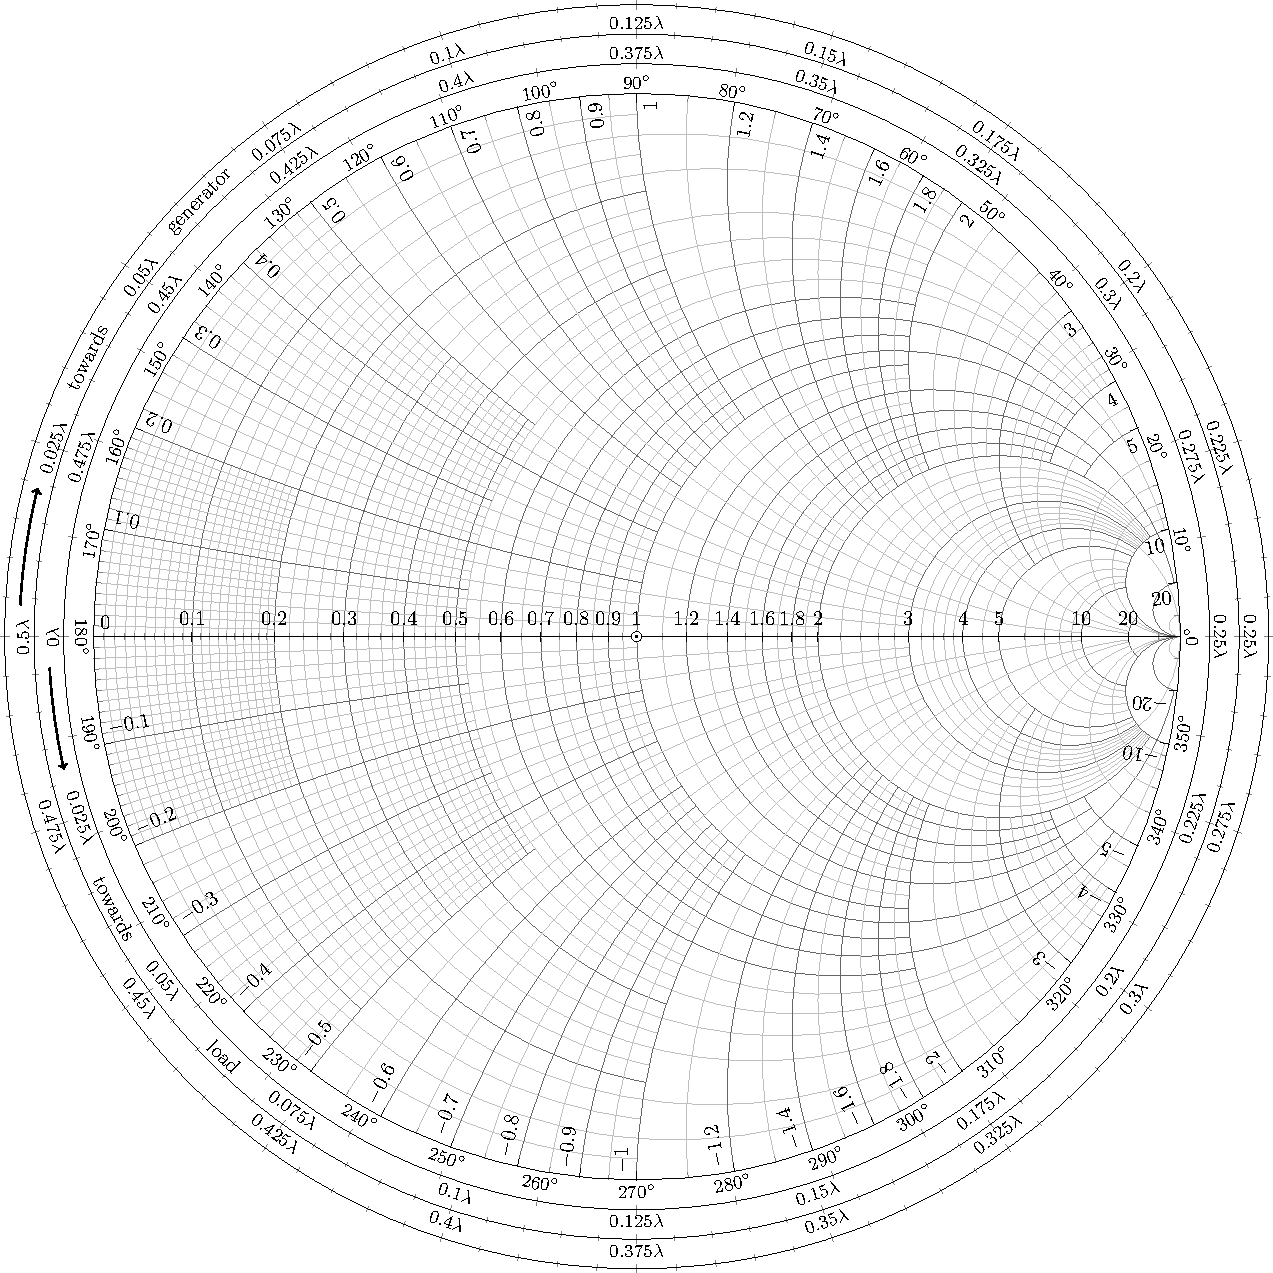
\includegraphics[width=6.5cm]{Cha4//SCexample1-eps-converted-to.pdf}}
      \only<2>{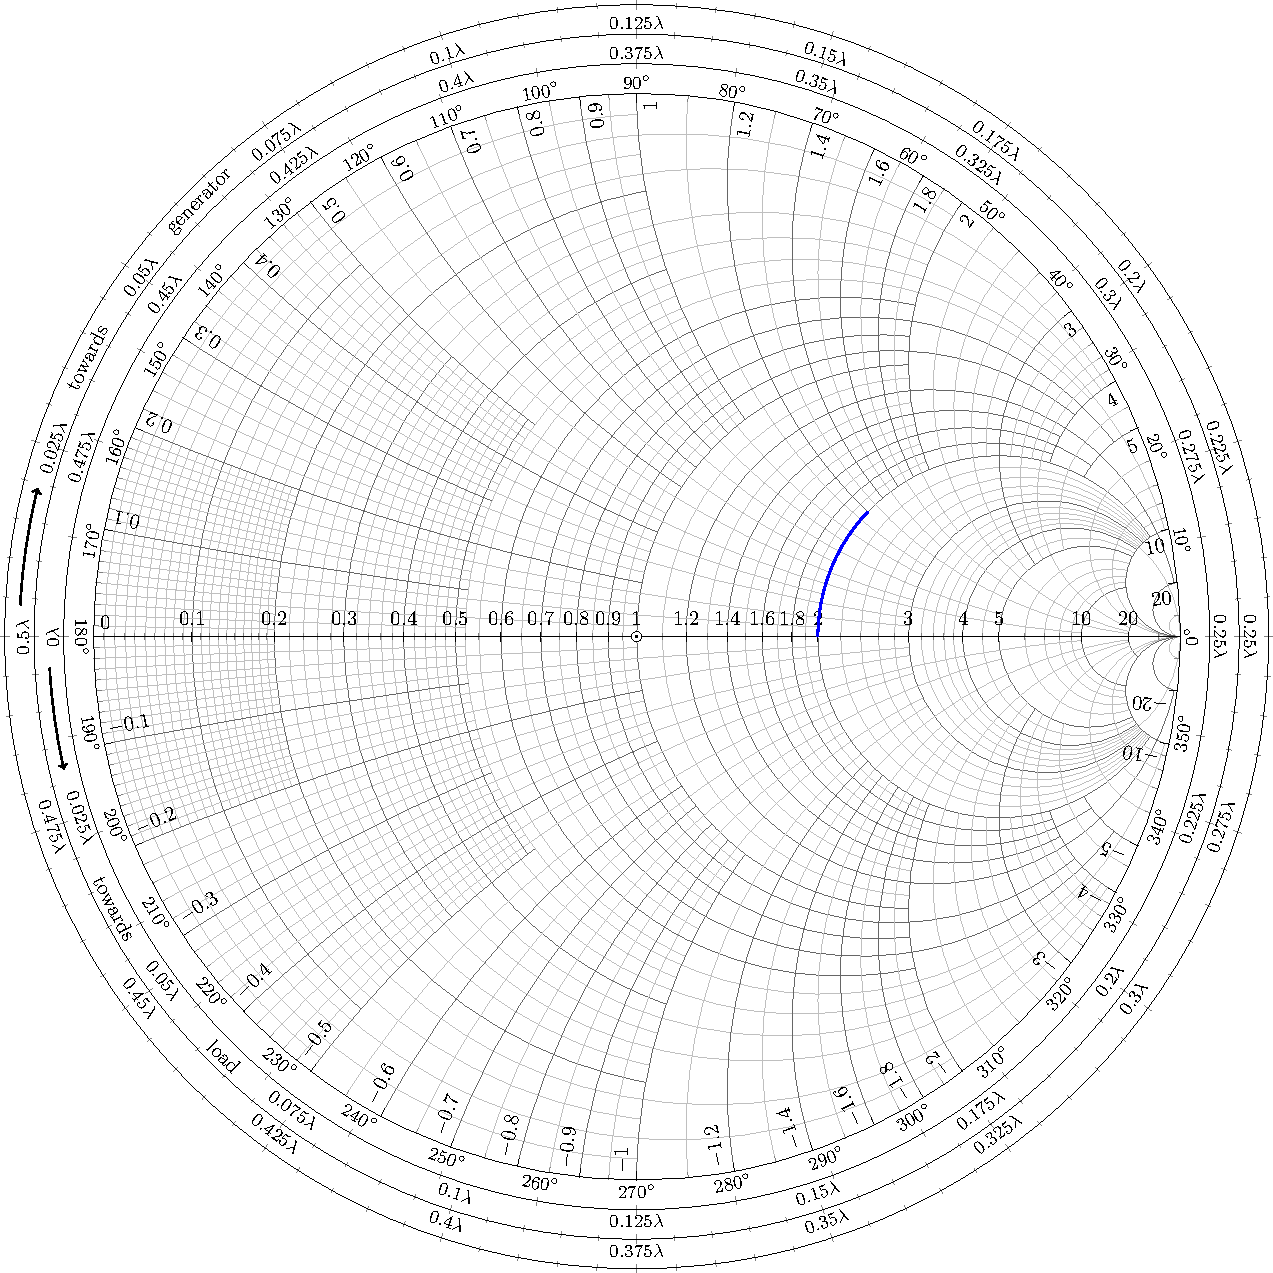
\includegraphics[width=6.5cm]{Cha4//SCexample2-eps-converted-to.pdf}}
      \only<3>{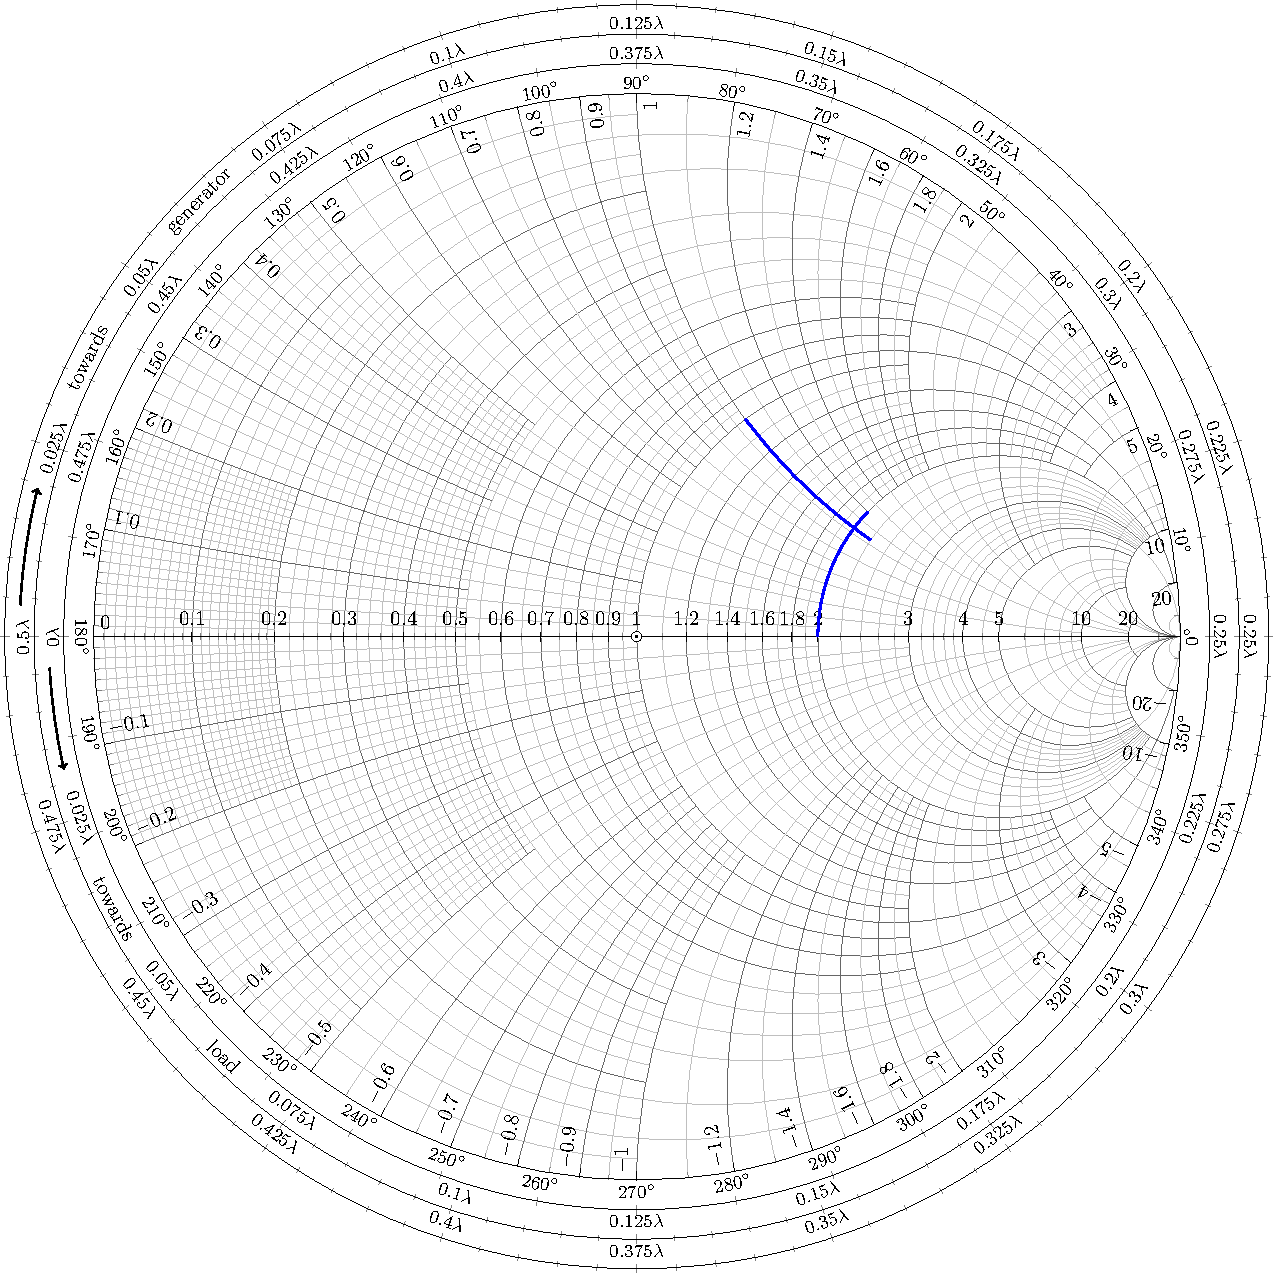
\includegraphics[width=6.5cm]{Cha4//SCexample3-eps-converted-to.pdf}}
      \only<4>{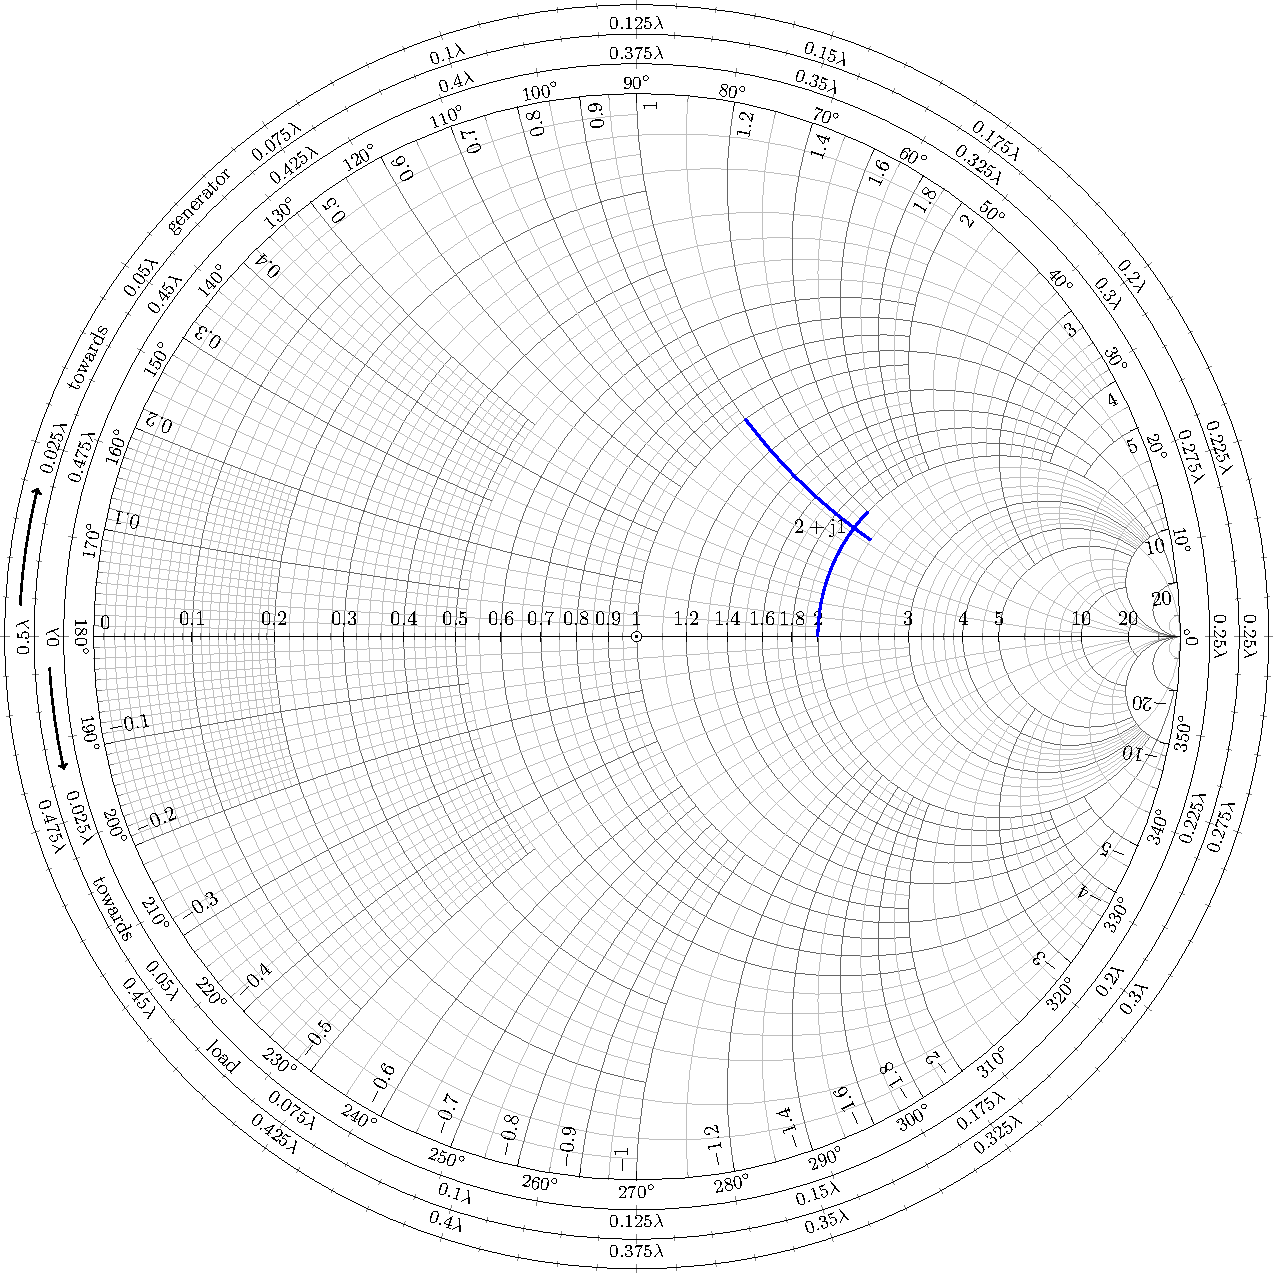
\includegraphics[width=6.5cm]{Cha4//SCexample4-eps-converted-to.pdf}}
      \only<5>{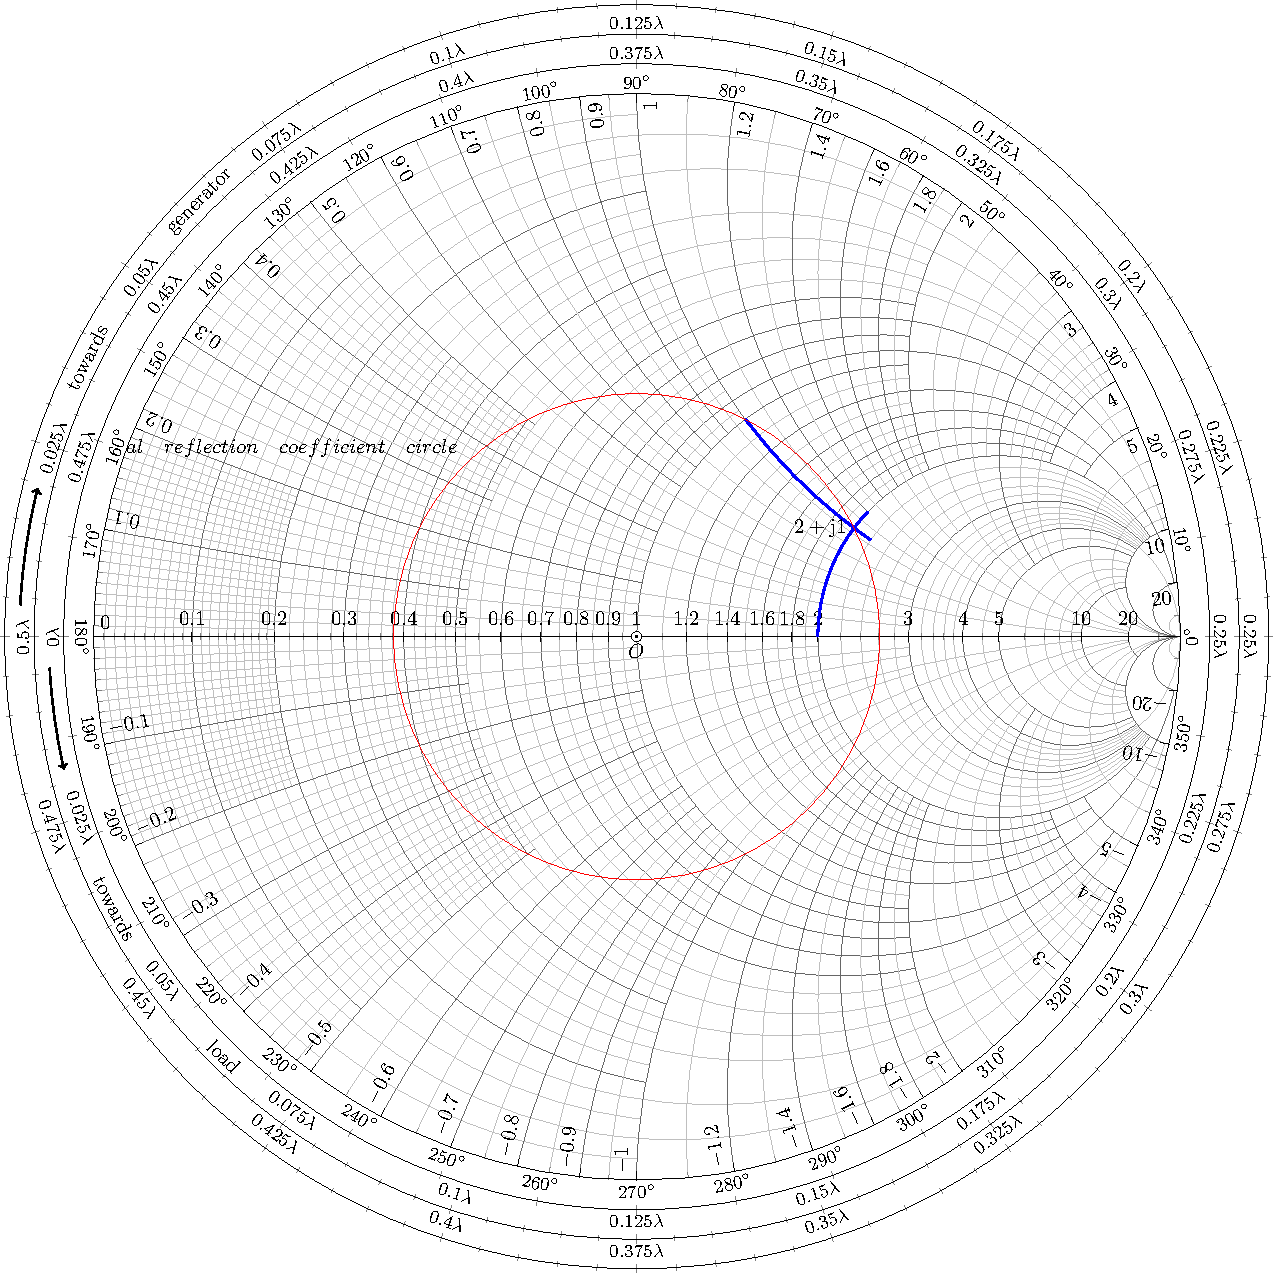
\includegraphics[width=6.5cm]{Cha4//SCexample5-eps-converted-to.pdf}}
      \only<6>{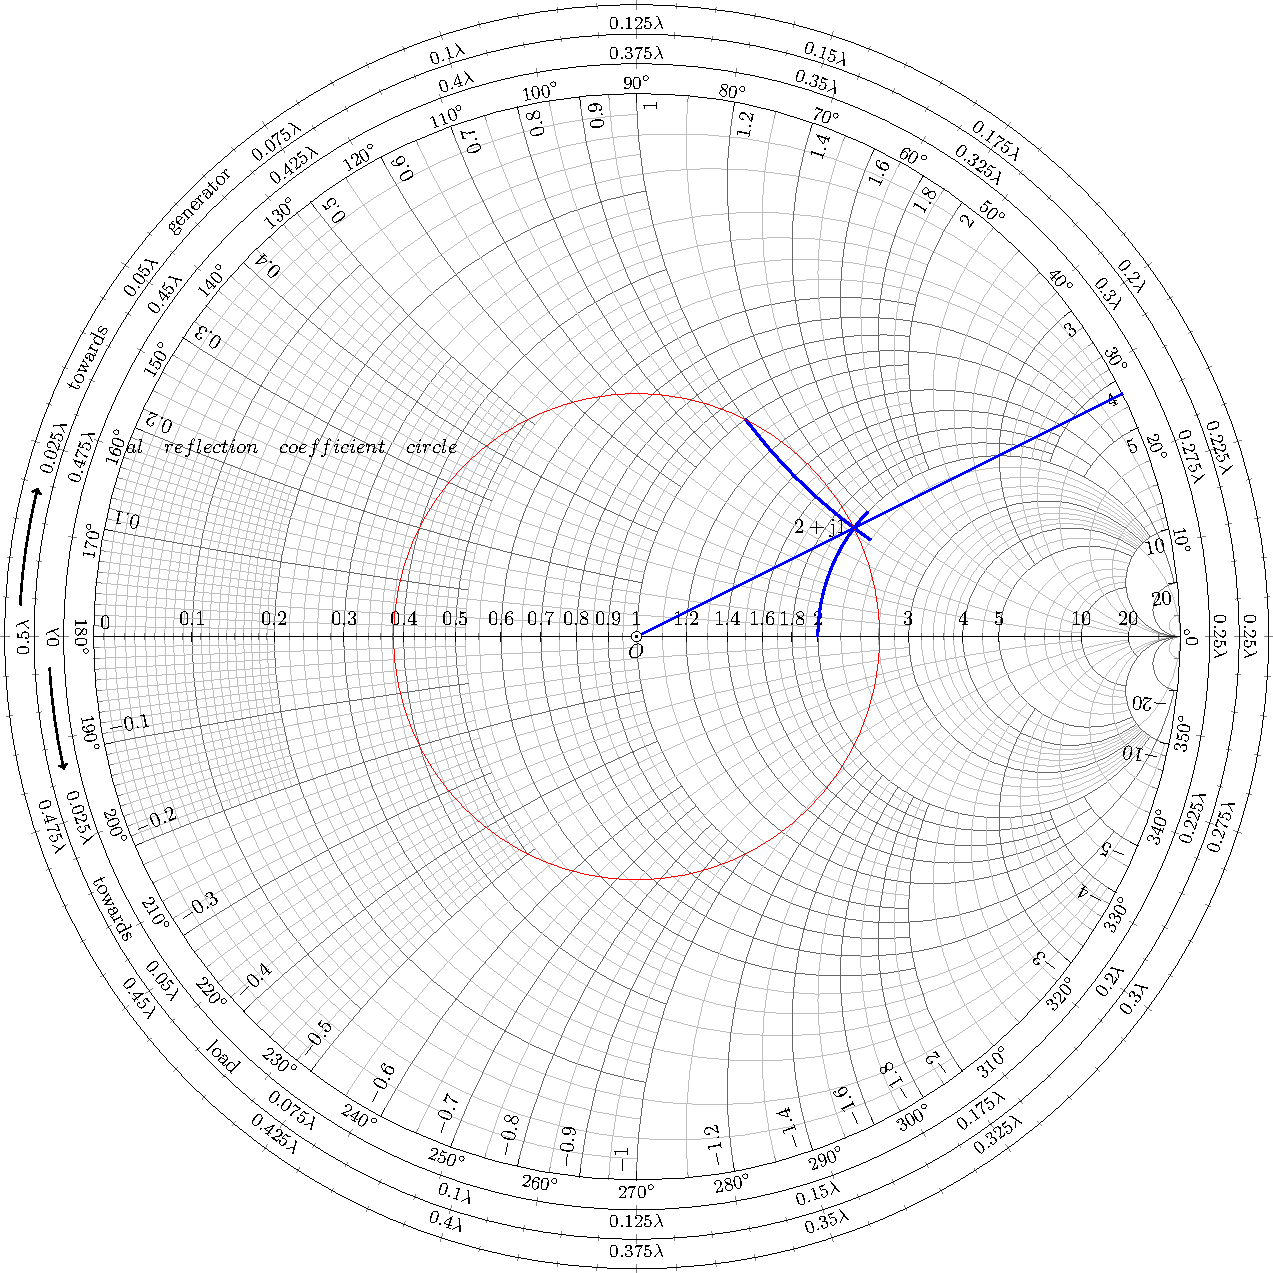
\includegraphics[width=6.5cm]{Cha4//SCexample6-eps-converted-to.pdf}}
      \only<7>{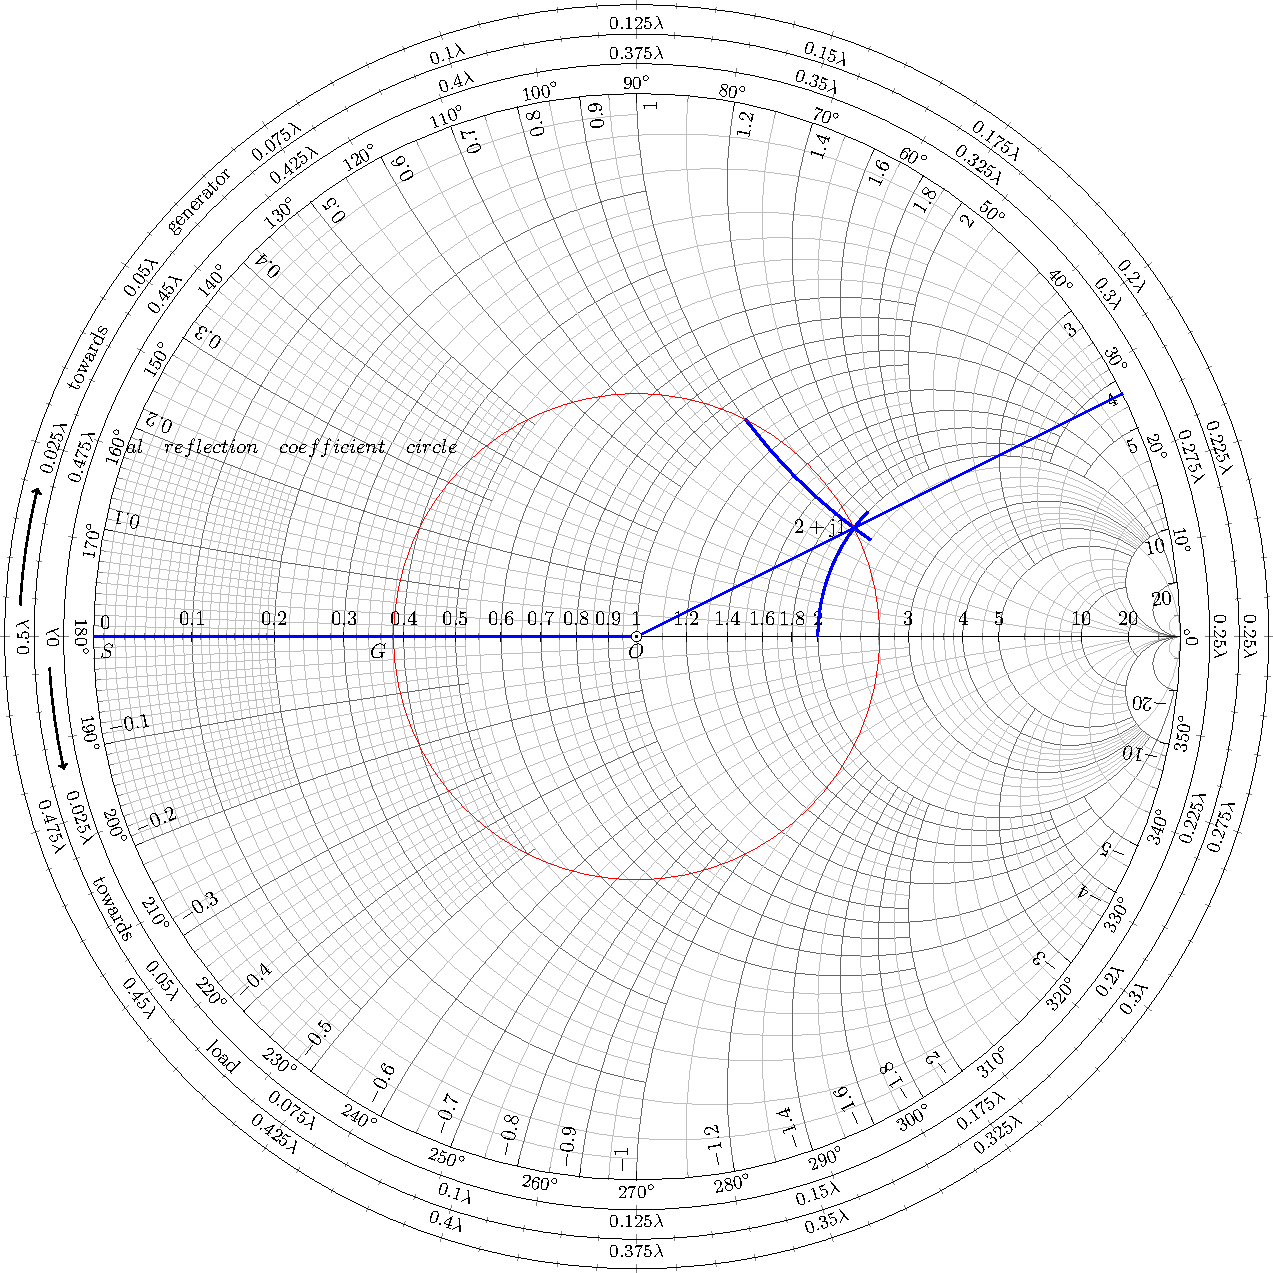
\includegraphics[width=6.5cm]{Cha4//SCexample7-eps-converted-to.pdf}}
      \only<8>{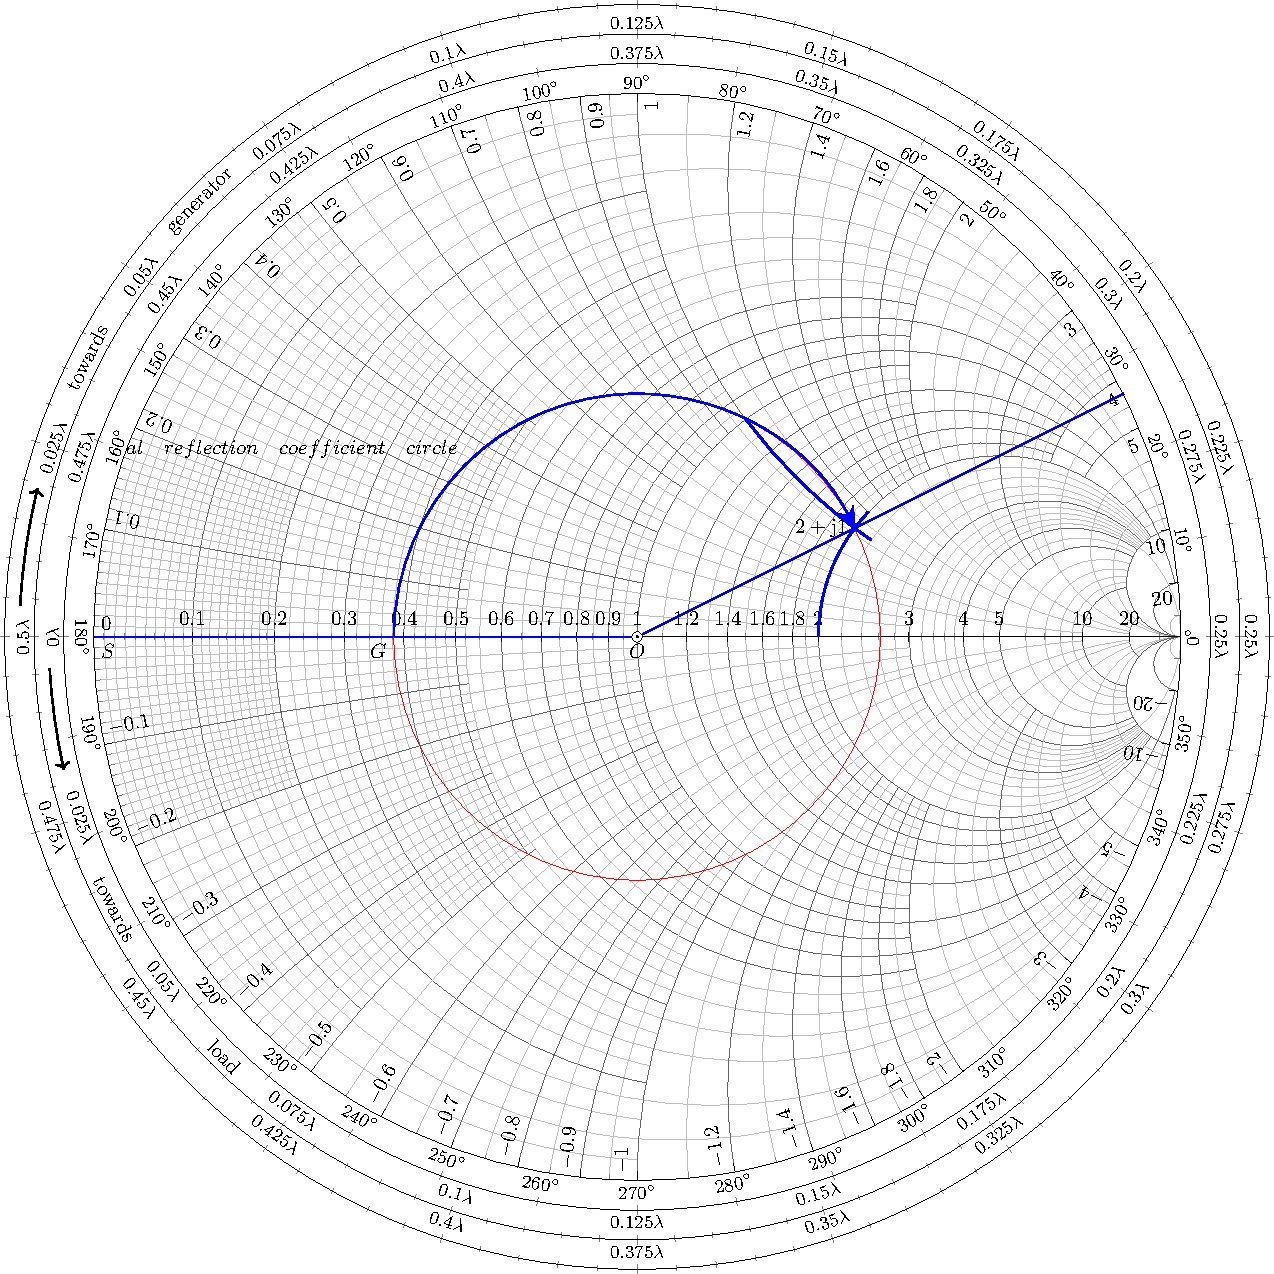
\includegraphics[width=6.5cm]{Cha4//fig4-10-8.pdf}}
      \only<9>{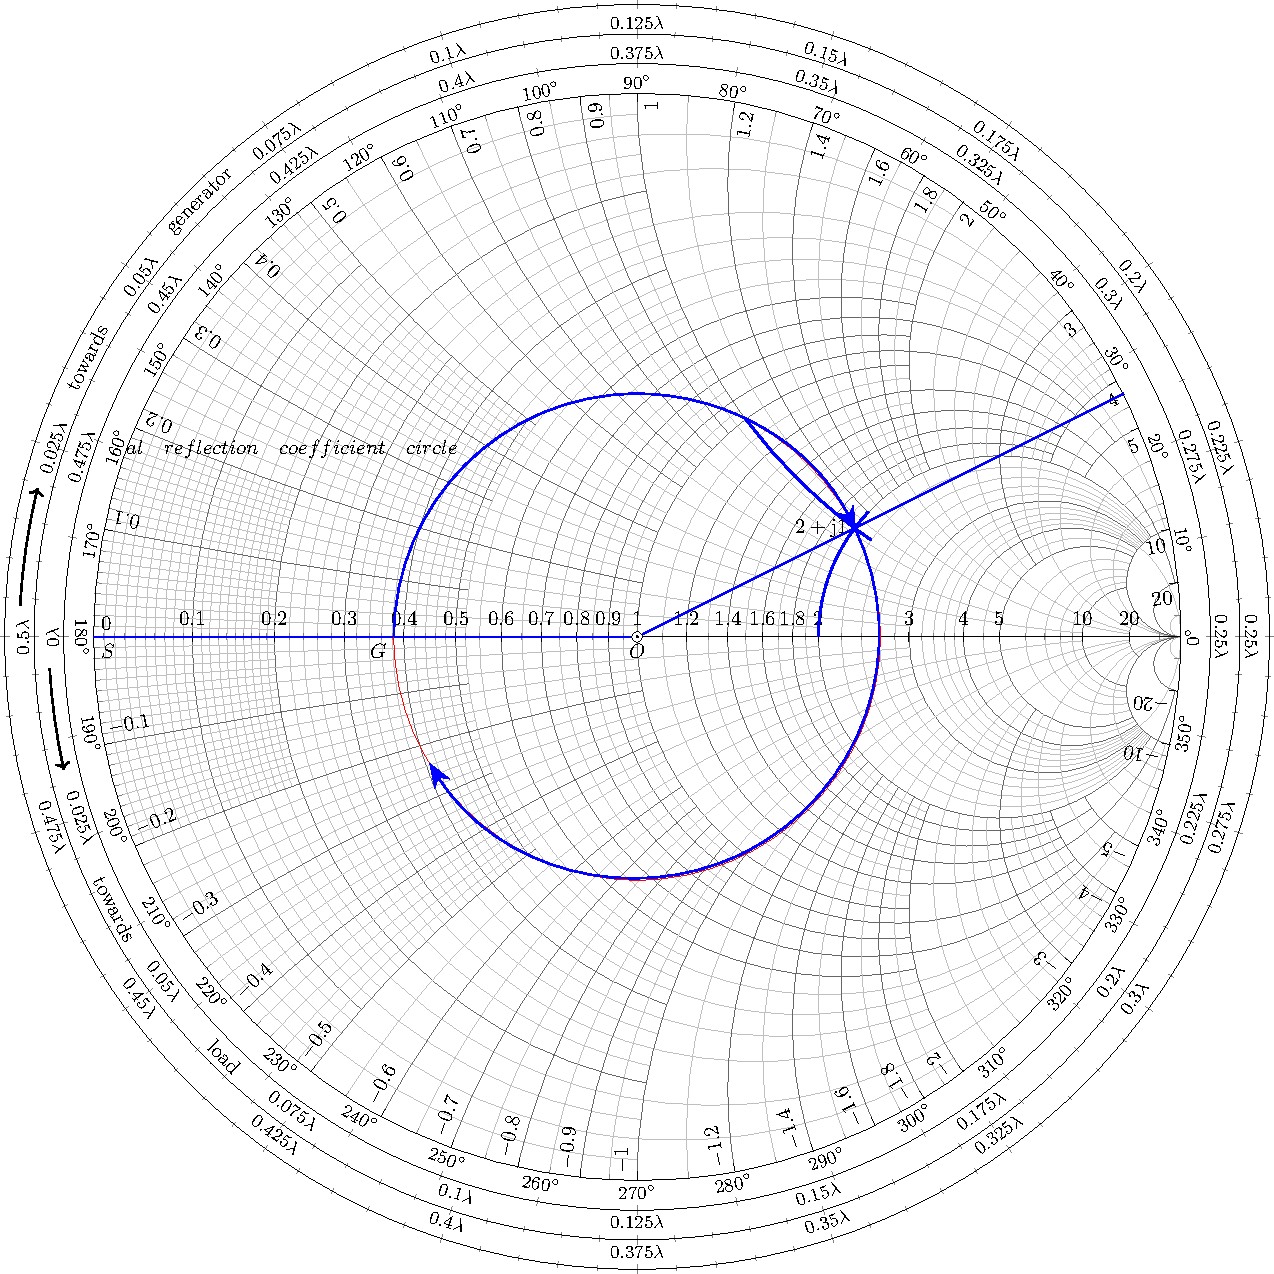
\includegraphics[width=6.5cm]{Cha4//fig4-10-9.pdf}}
      \only<10>{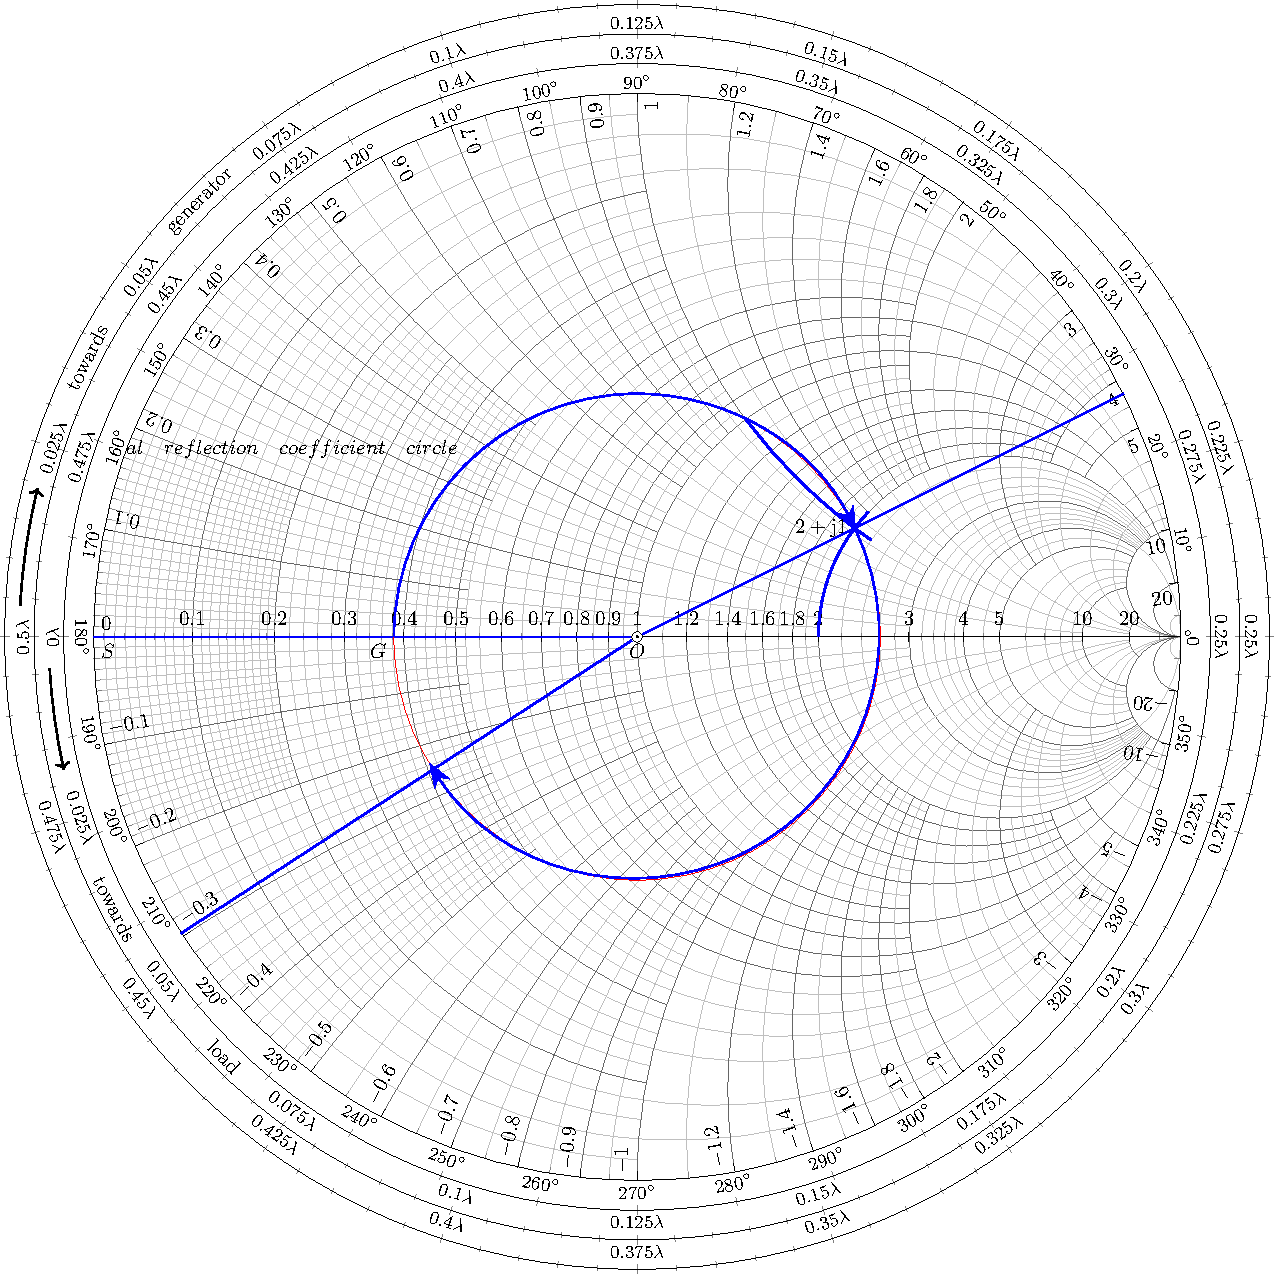
\includegraphics[width=6.5cm]{Cha4//fig4-10-10.pdf}}
      \only<11>{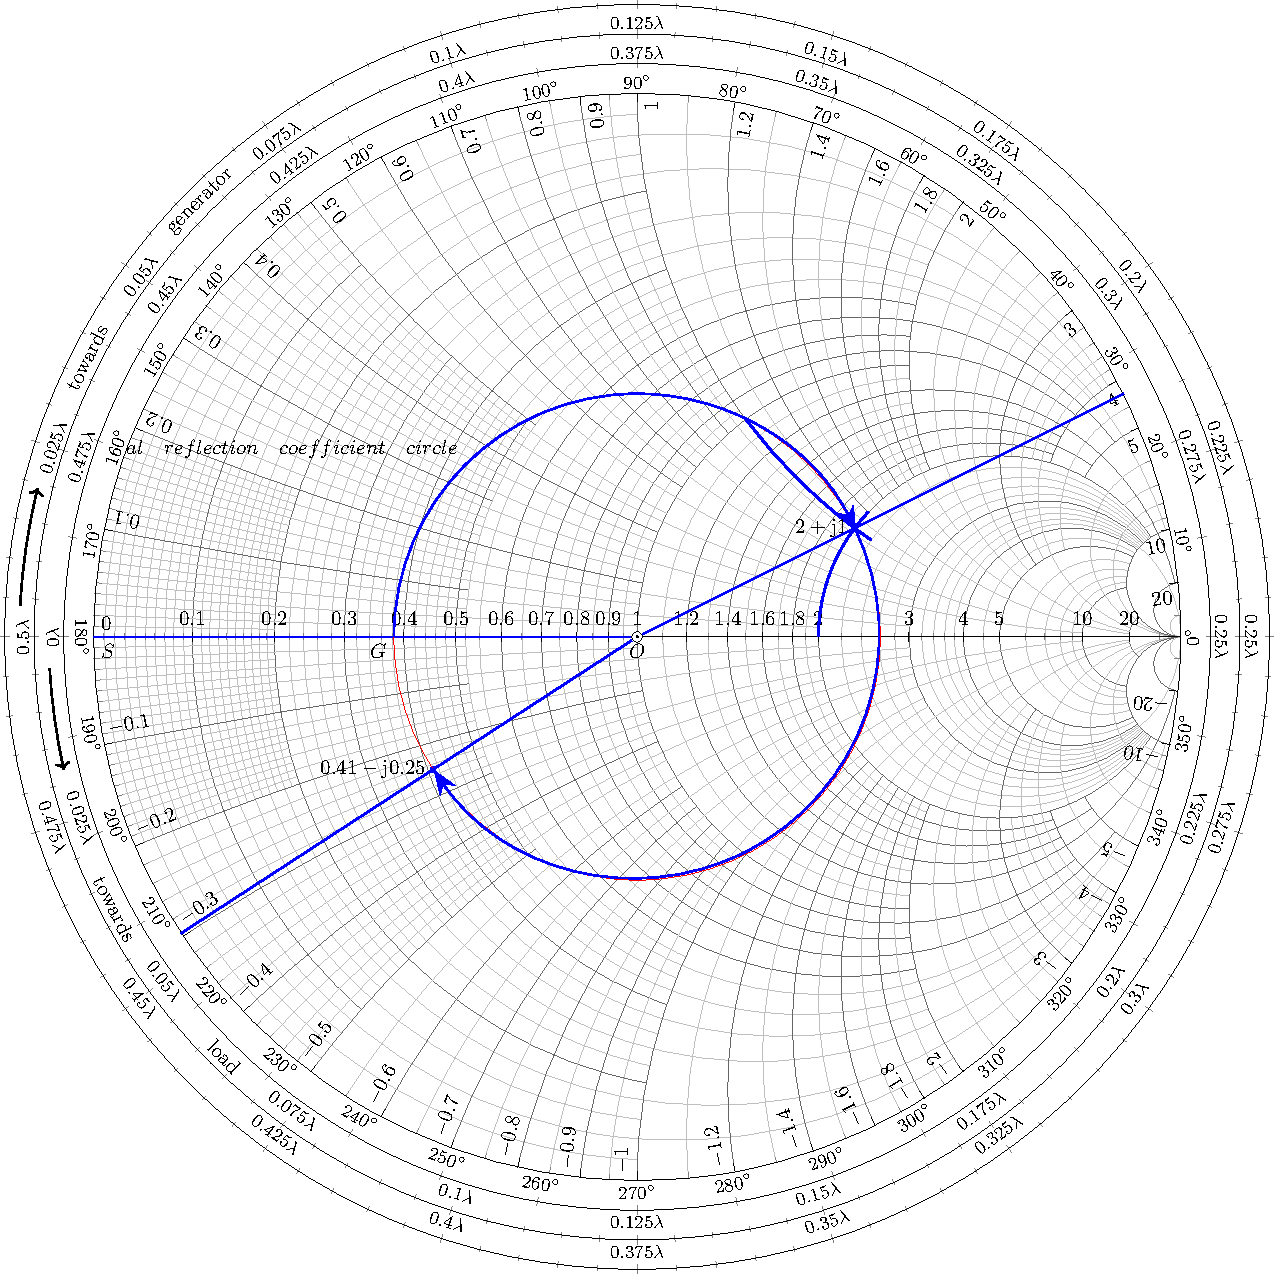
\includegraphics[width=6.5cm]{Cha4//fig4-10-11.pdf}}

      %\only<1>{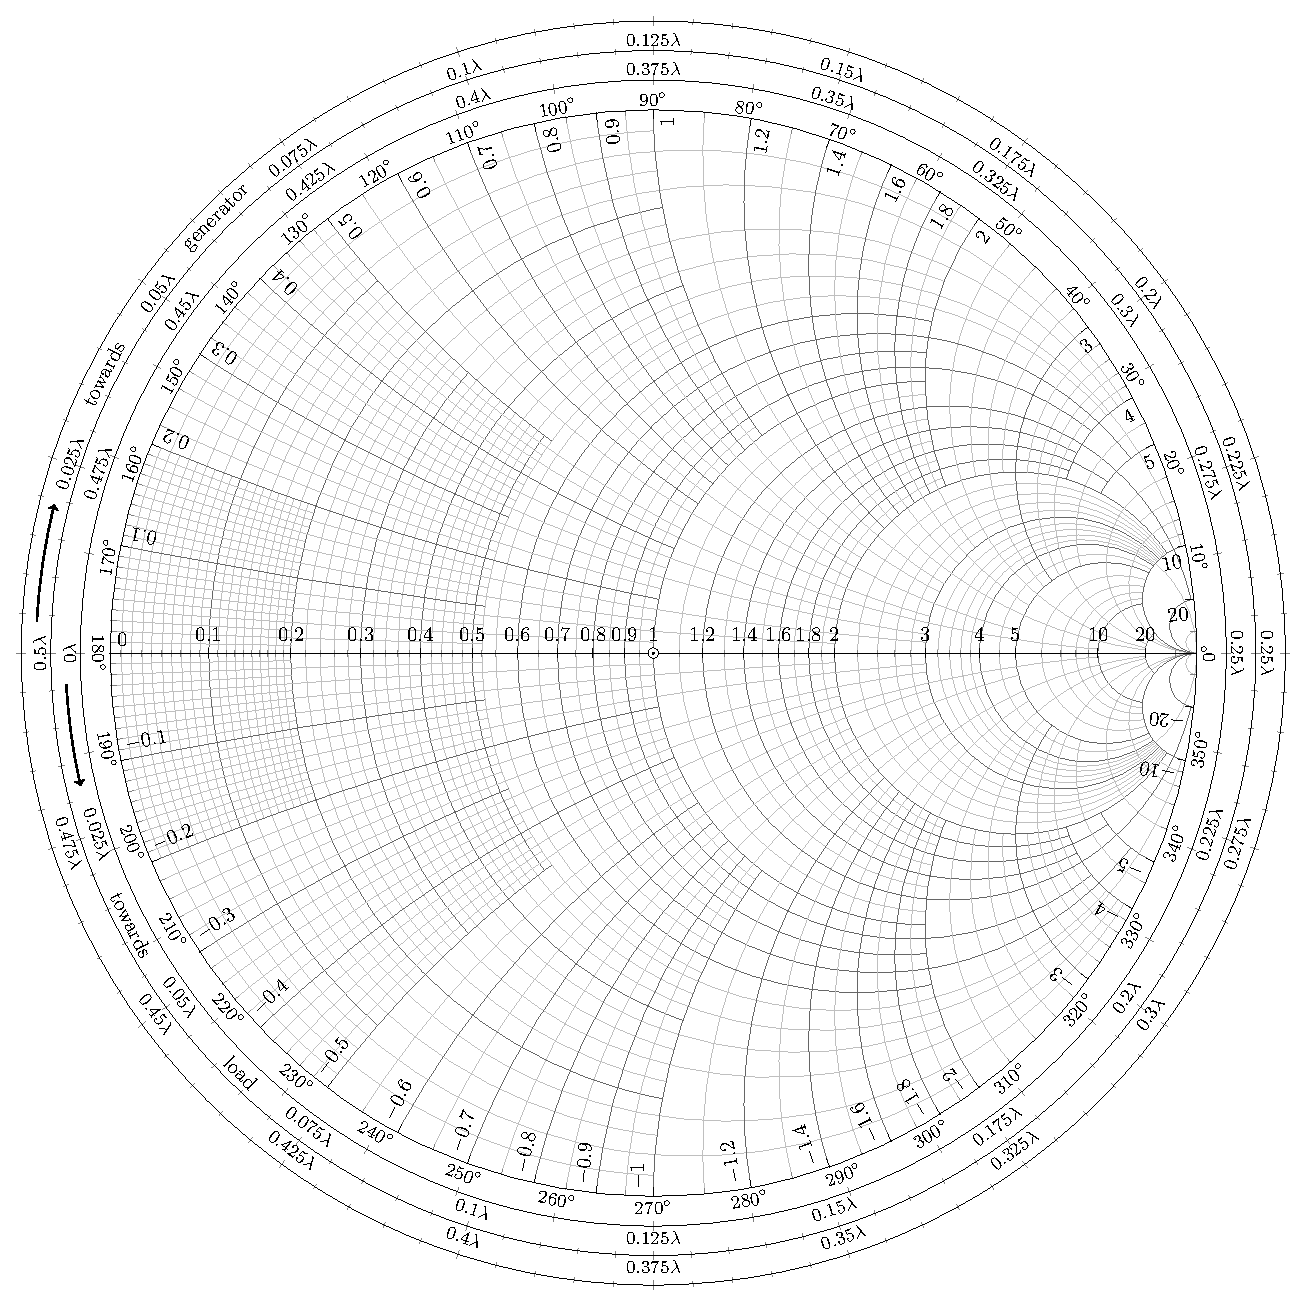
\includegraphics[width=6cm]{SCexample1.eps}}
    \end{column}
  \end{columns}
\end{frame}

\begin{frame}{Smith圆图的应用}
  例2 \quad 已知无耗传输线的特征阻抗为$50\Omega$,长度为$0.1\lambda$,终端短路,求输入阻抗。
  \begin{columns}
    \begin{column}{0.4\linewidth}
      1)\quad 先找出终端短路点$S$\\
      2)\quad 向源方向旋转$0.1\lambda$,到圆图上$A$点,读出$x=0.72$
      \begin{flalign*}
        Z_{in}=Z_0z_{in} & =50\times\mathrm{j}0.72 \\
                         & =\mathrm{j}36\Omega
      \end{flalign*}
    \end{column}
    \begin{column}{0.6\linewidth}
      \only<1>{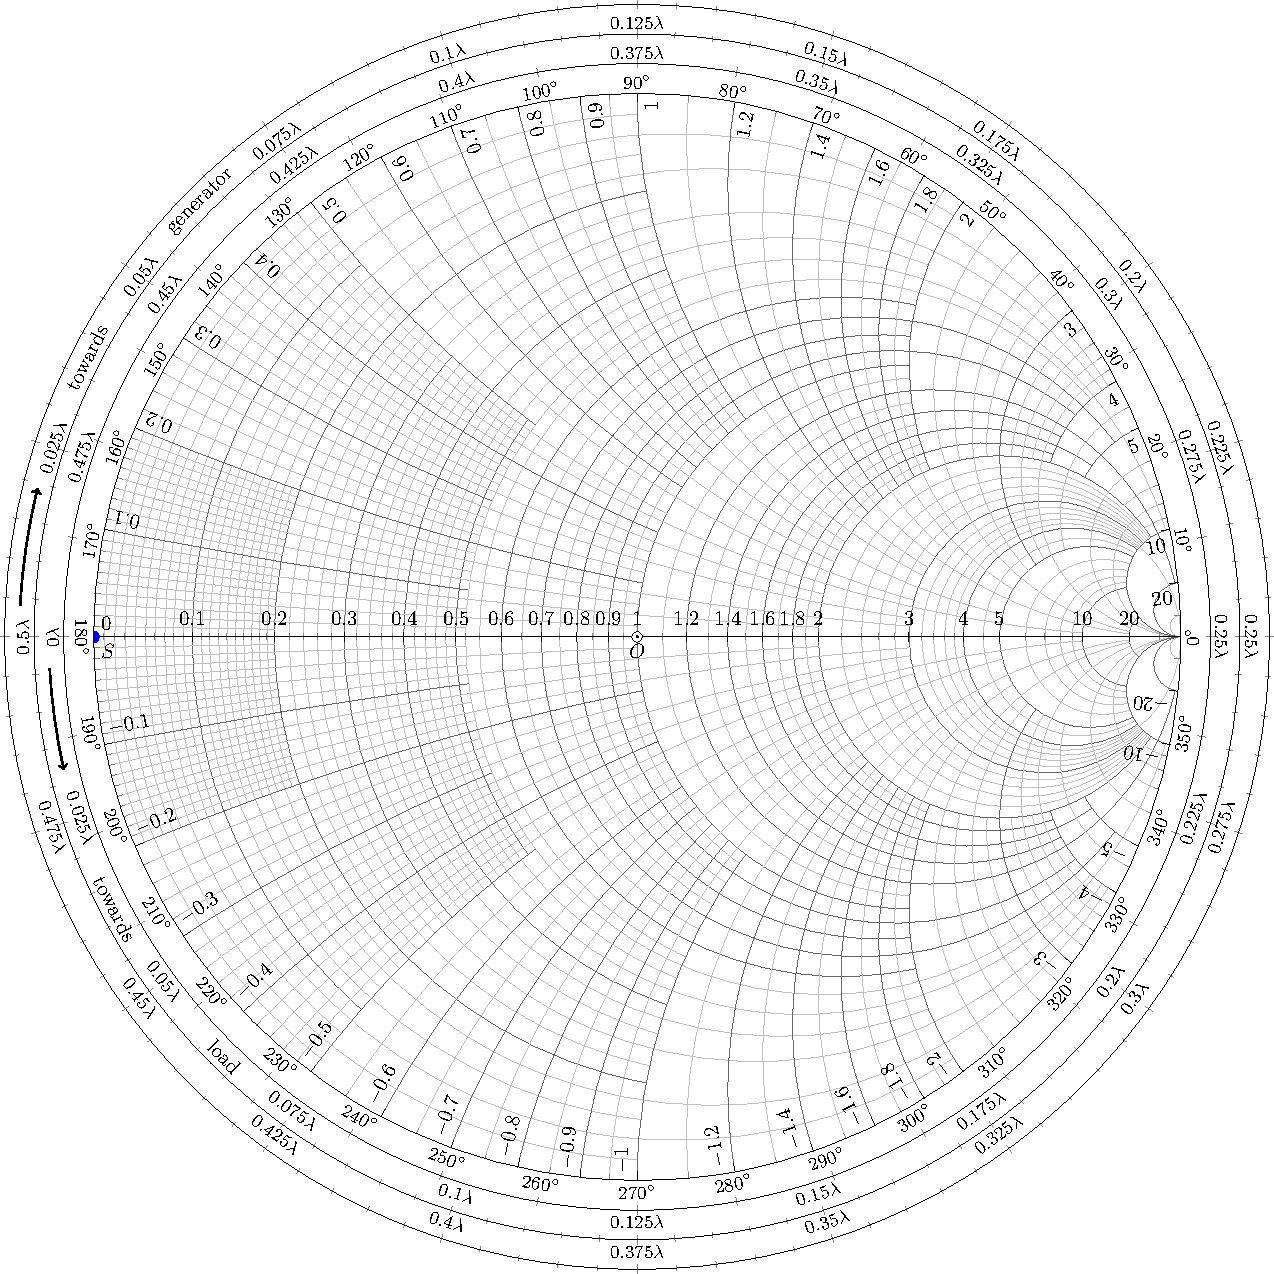
\includegraphics[width=6.5cm]{Cha4//fig4-11-1.pdf}}
      \only<2>{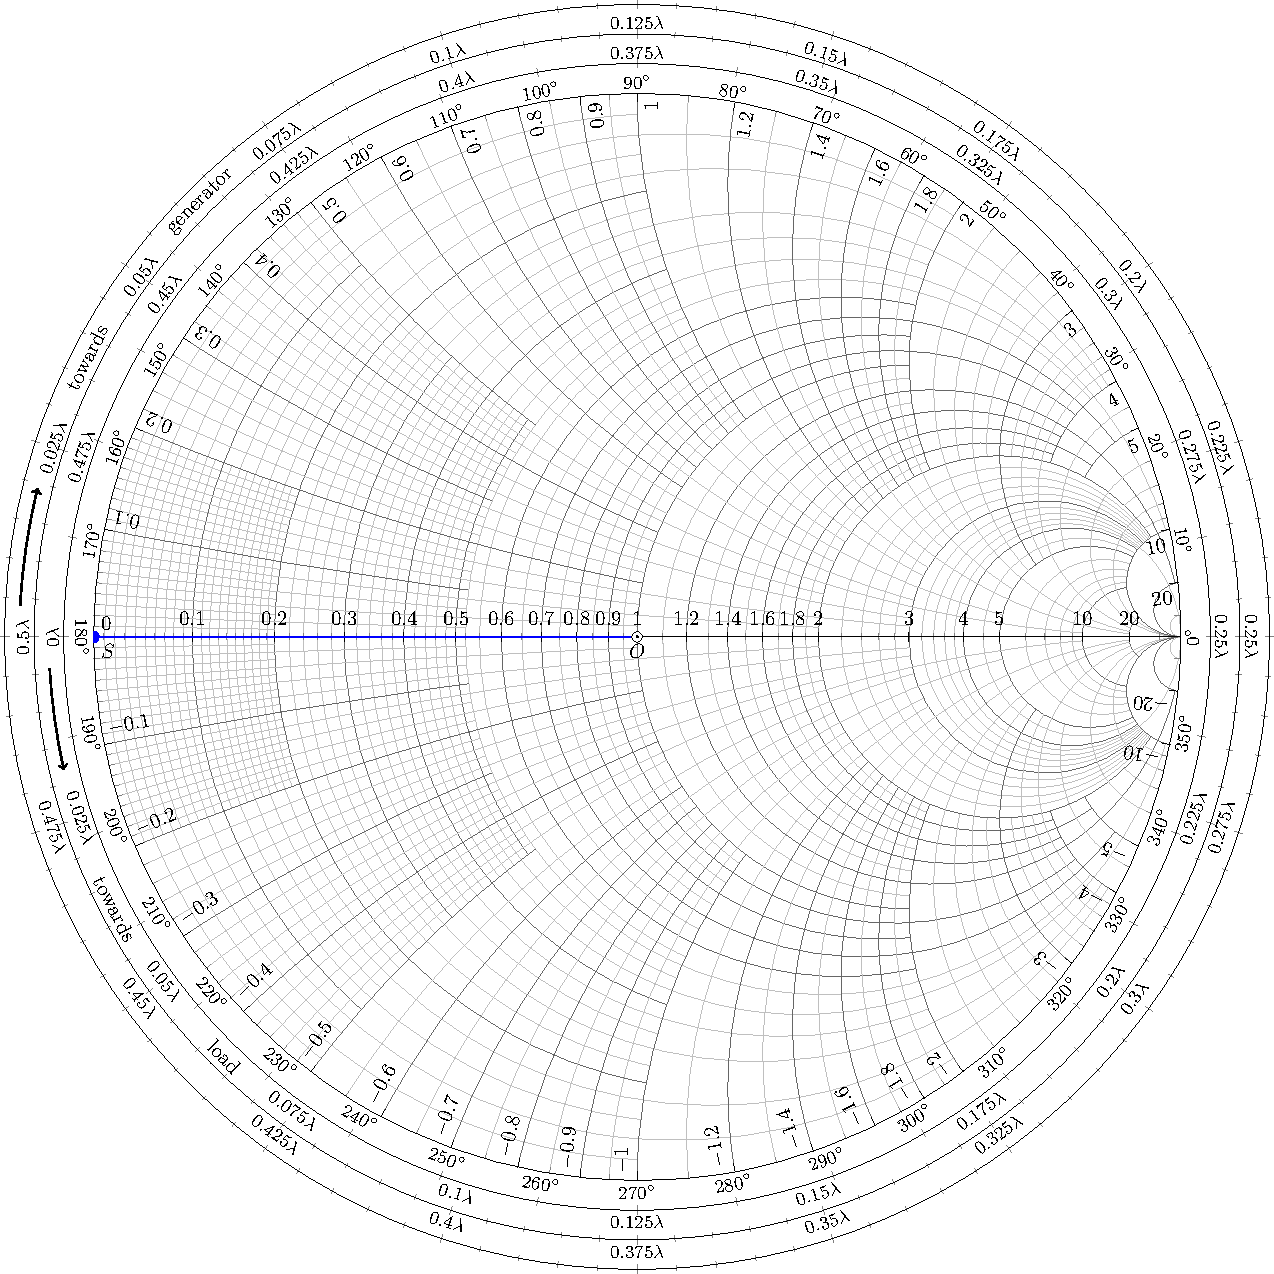
\includegraphics[width=6.5cm]{Cha4//fig4-11-2.pdf}}
      \only<3>{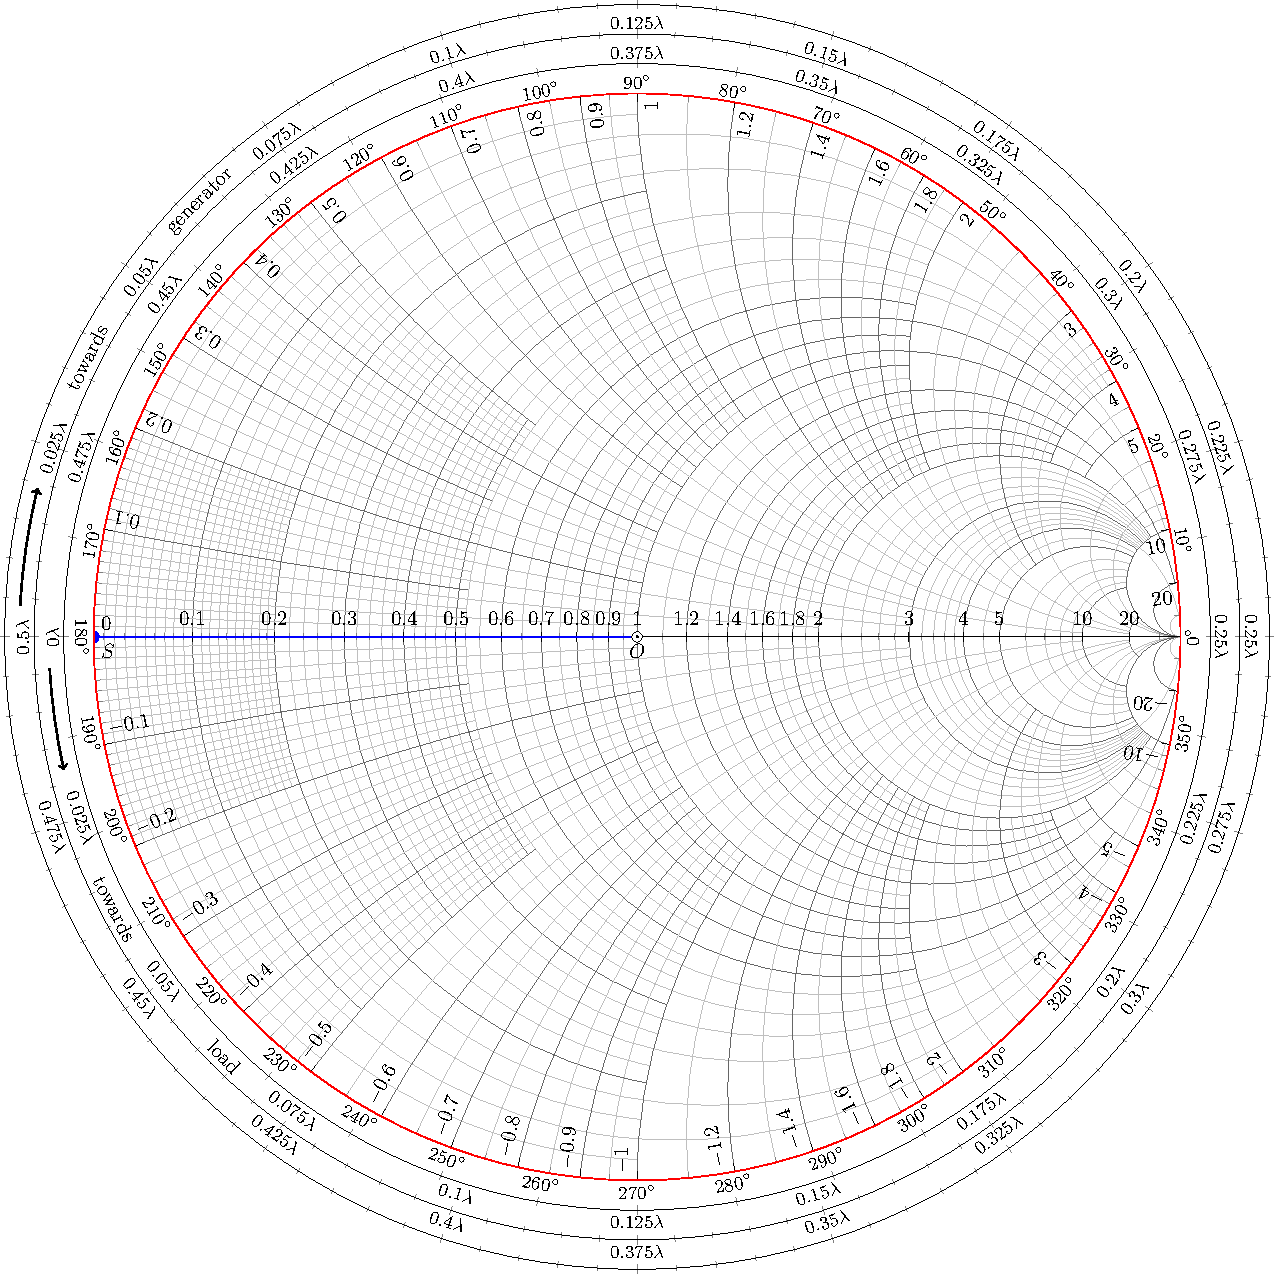
\includegraphics[width=6.5cm]{Cha4//fig4-11-3.pdf}}
      \only<4>{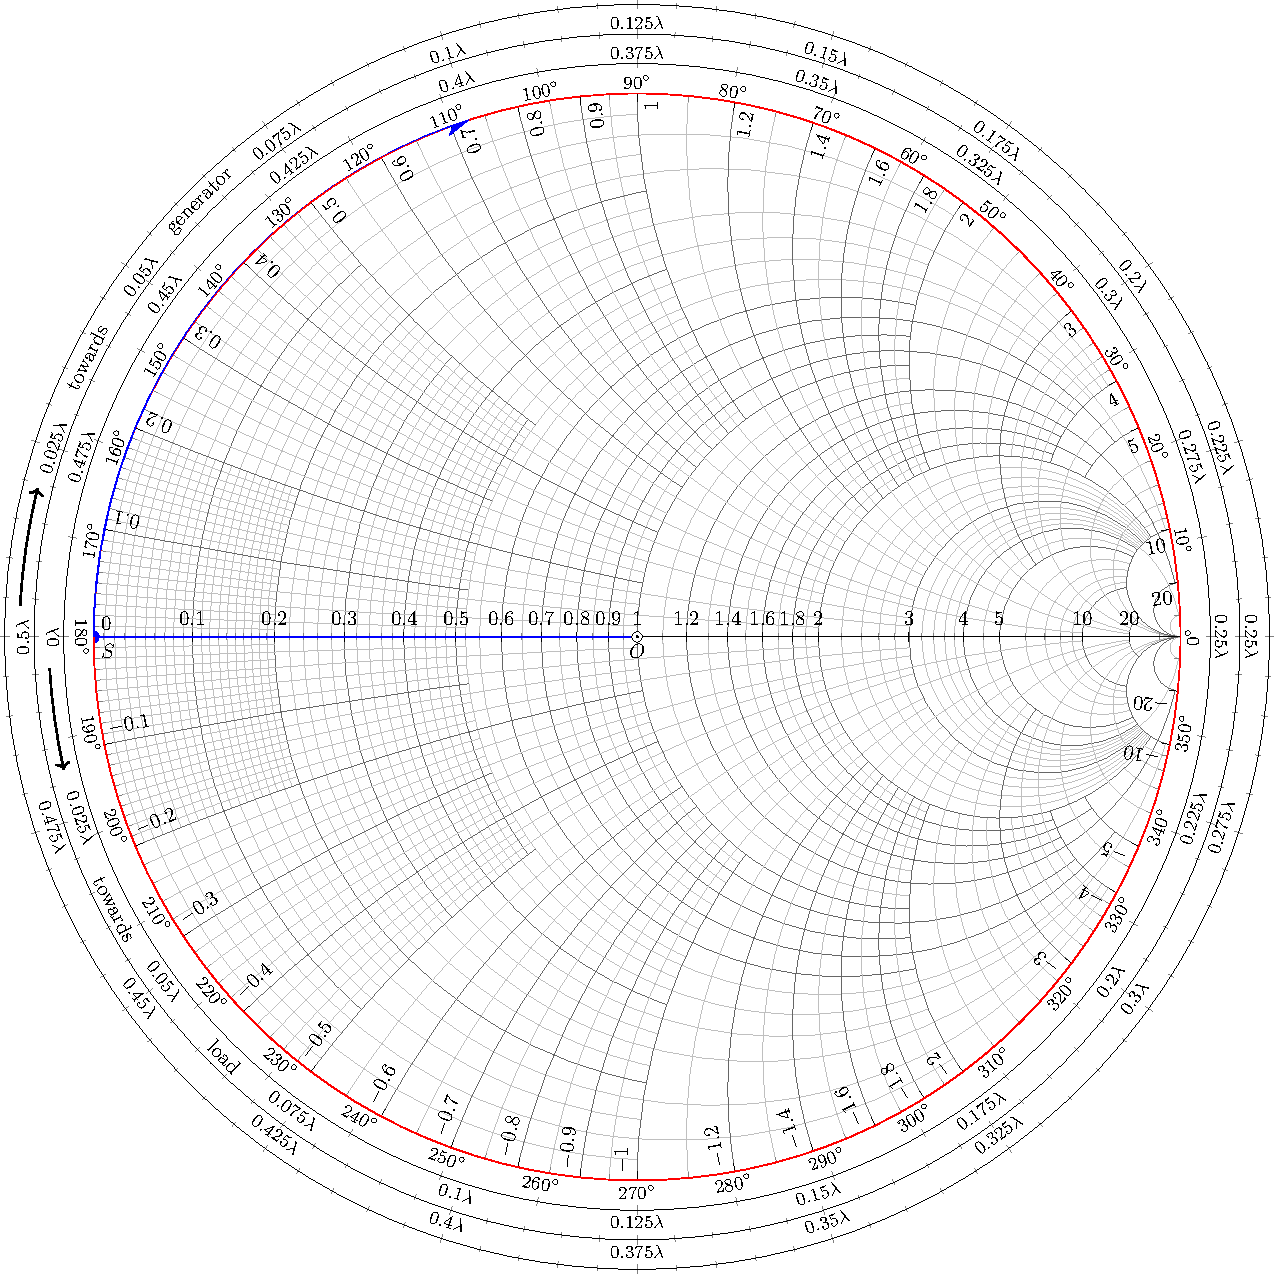
\includegraphics[width=6.5cm]{Cha4//fig4-11-4.pdf}}
      \only<5>{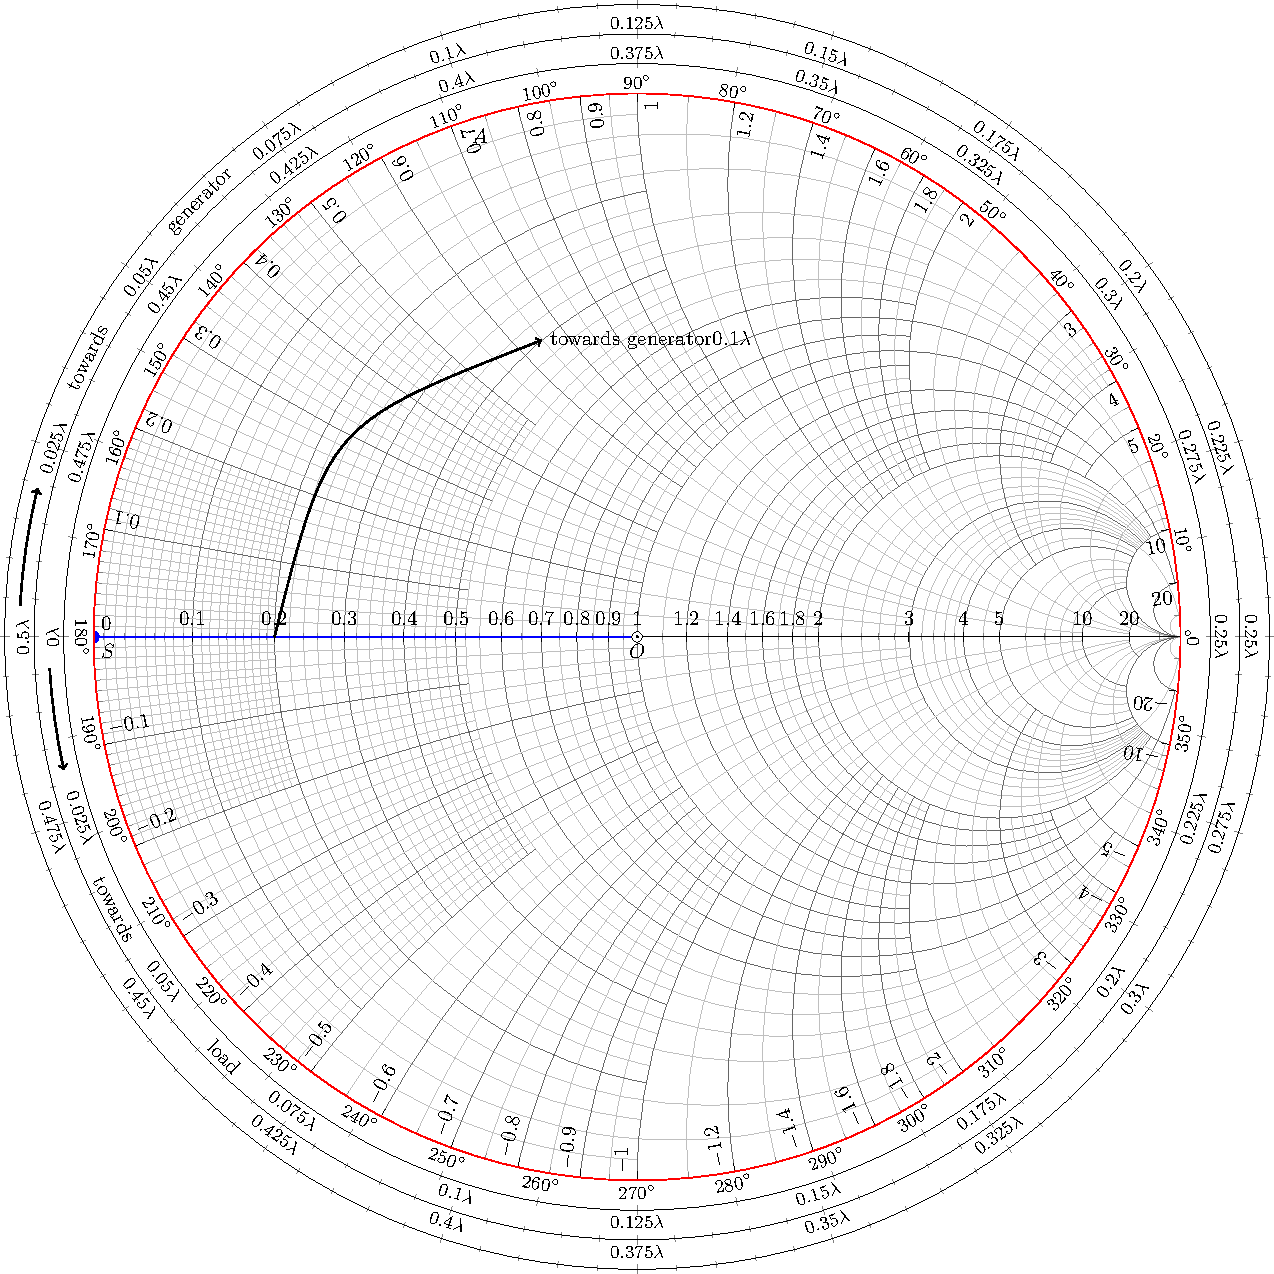
\includegraphics[width=6.5cm]{Cha4//fig4-11-5.pdf}}
      \only<6>{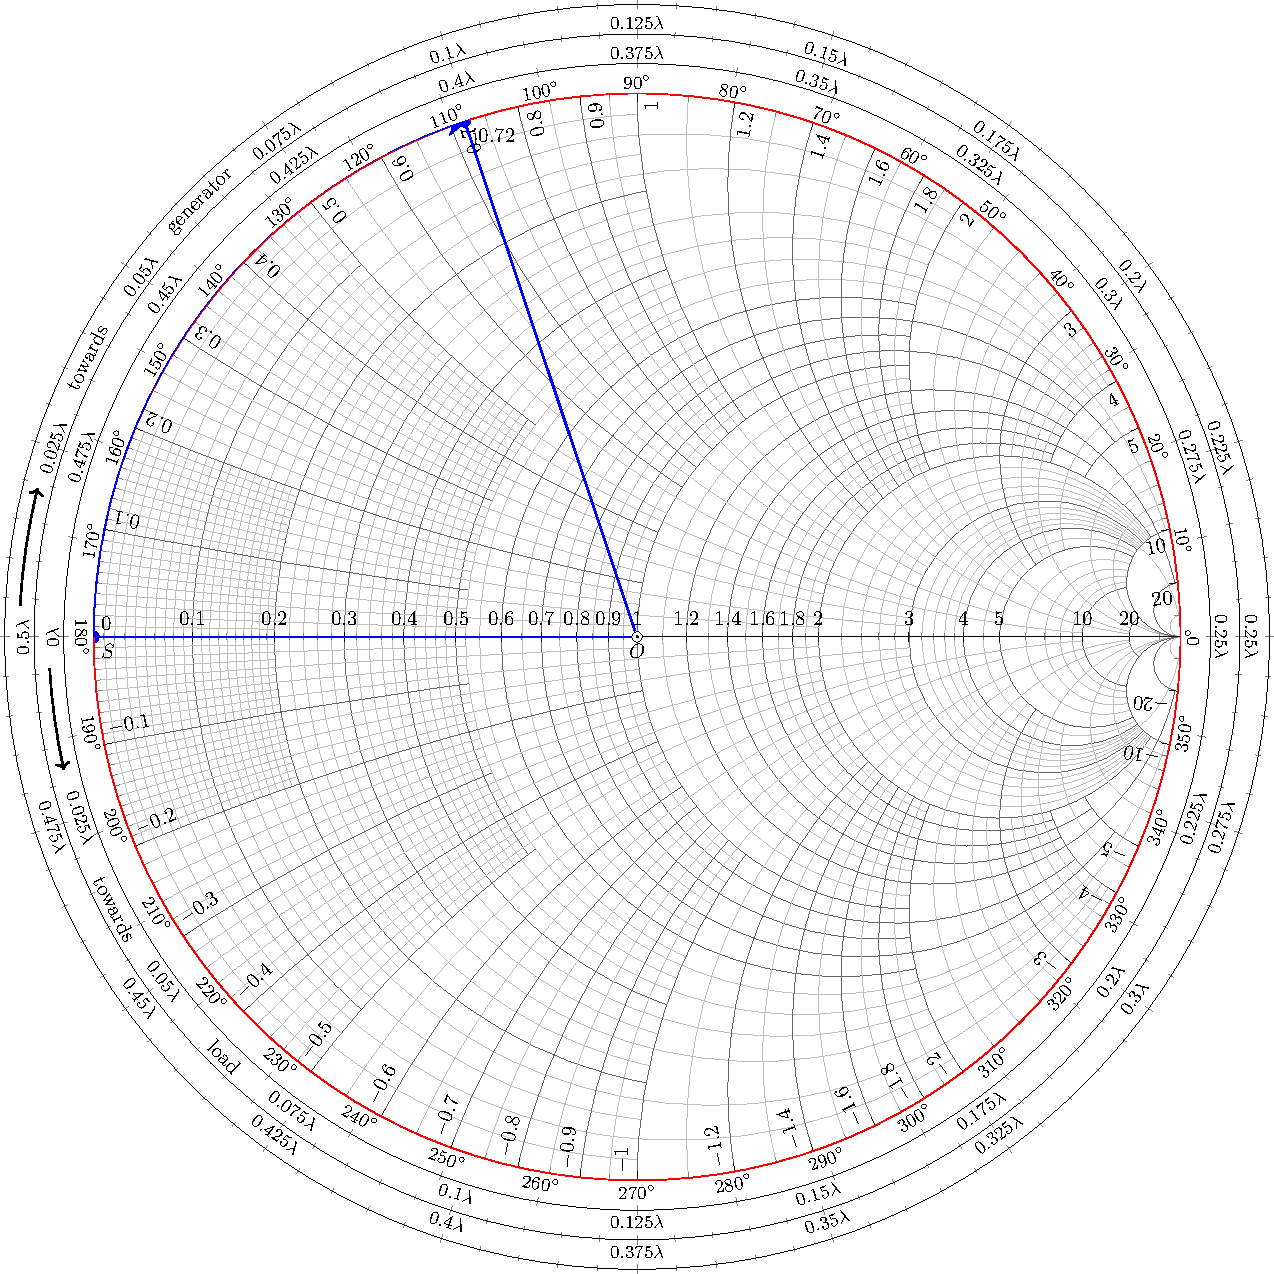
\includegraphics[width=6.5cm]{Cha4//fig4-11-6.pdf}}
    \end{column}
  \end{columns}
\end{frame}

\begin{frame}{Smith圆图的应用}
  例3 \quad 已知无耗传输线的特征阻抗为$Z_0=50\Omega$,端接负载阻抗为$Z_L=(85+\mathrm{j}30)\Omega$,利用圆图求驻波比。
  \begin{columns}
    \begin{column}{0.4\linewidth}
      1)\quad 首先对负载归一化
      \begin{flalign*}
        z_L=\frac{Z_L}{Z_0}=1.7+\mathrm{j}0.6
      \end{flalign*}
      2)\quad 在$Smith$圆图中确定负载位置$A$点:$r=1.7,x=0.6$,并画出负载所在的等反射系数圆\\
      3)\quad 由图读出与等反射系数圆相切的电阻圆的$r$值即为驻波比 $\rho=2.0$
    \end{column}
    \begin{column}{0.6\linewidth}
      \only<1>{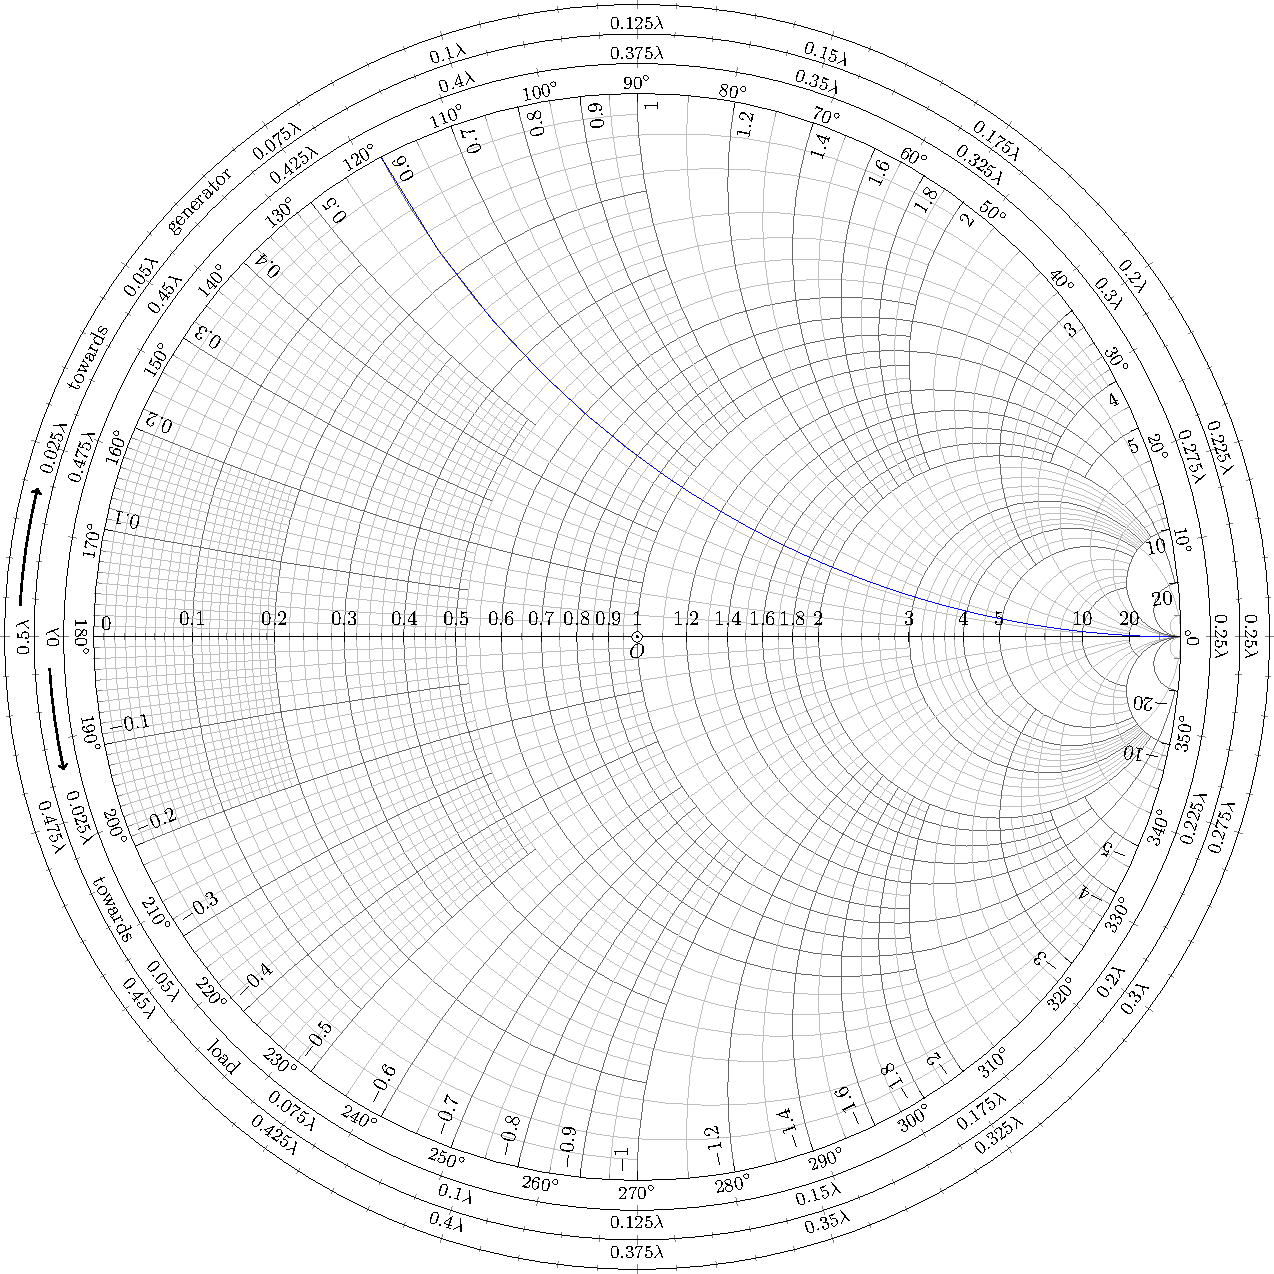
\includegraphics[width=7cm]{Cha4//fig4-12-1.pdf}}
      \only<2>{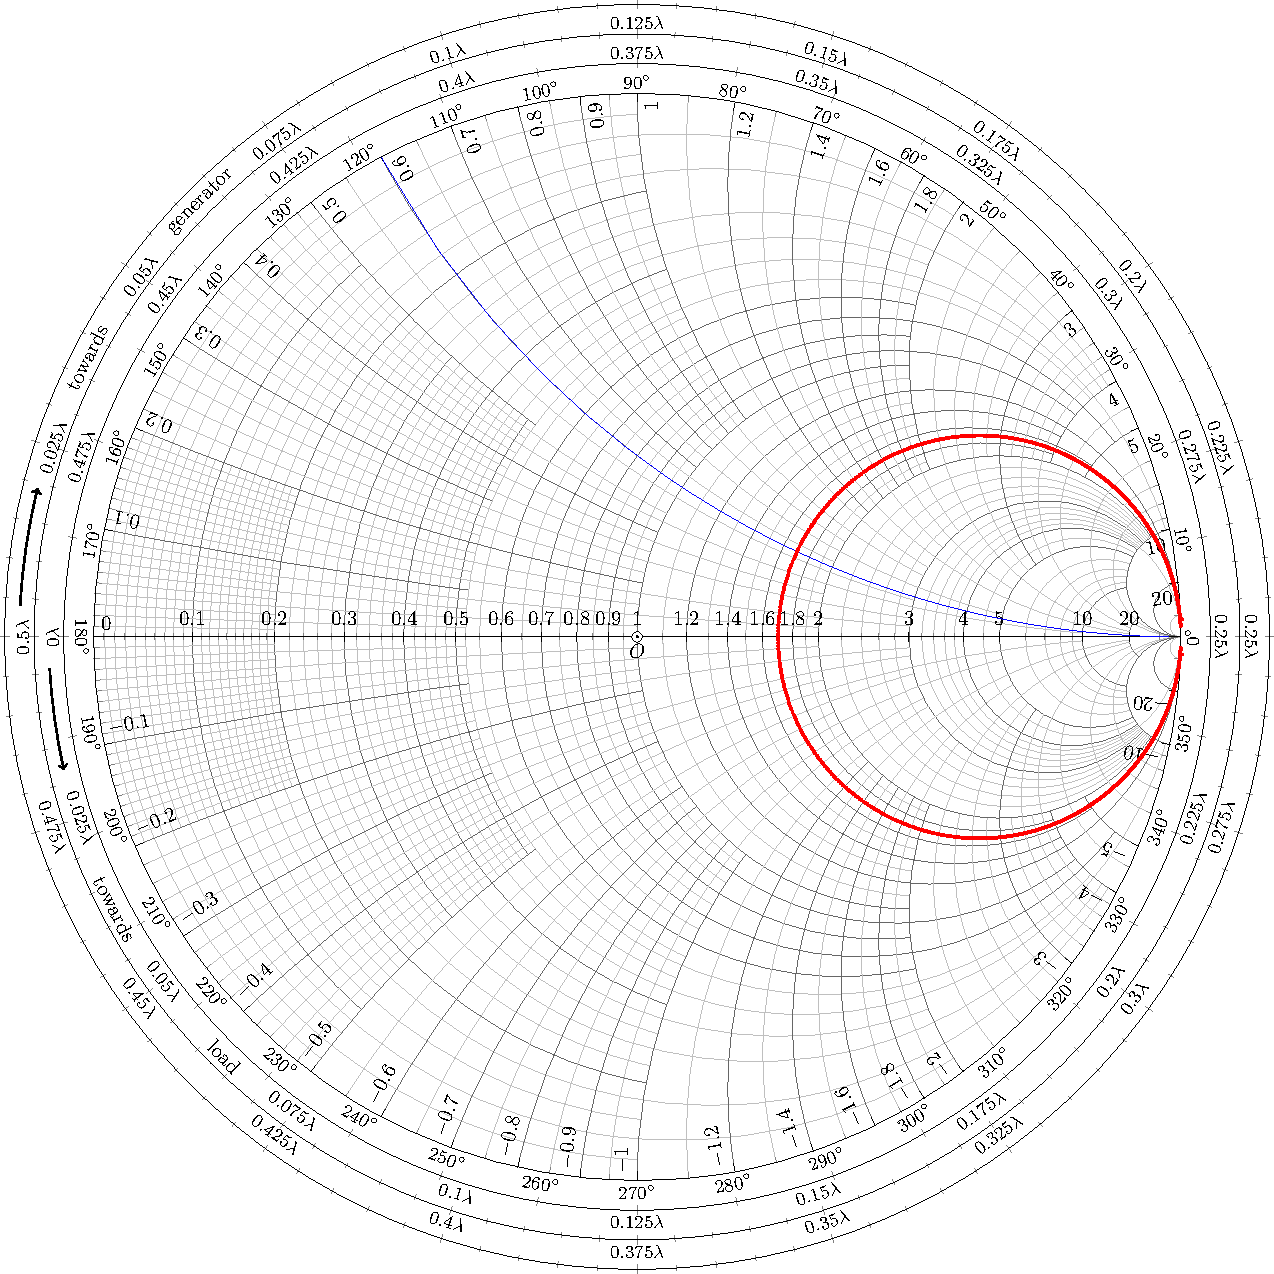
\includegraphics[width=7cm]{Cha4//fig4-12-2.pdf}}
      \only<3>{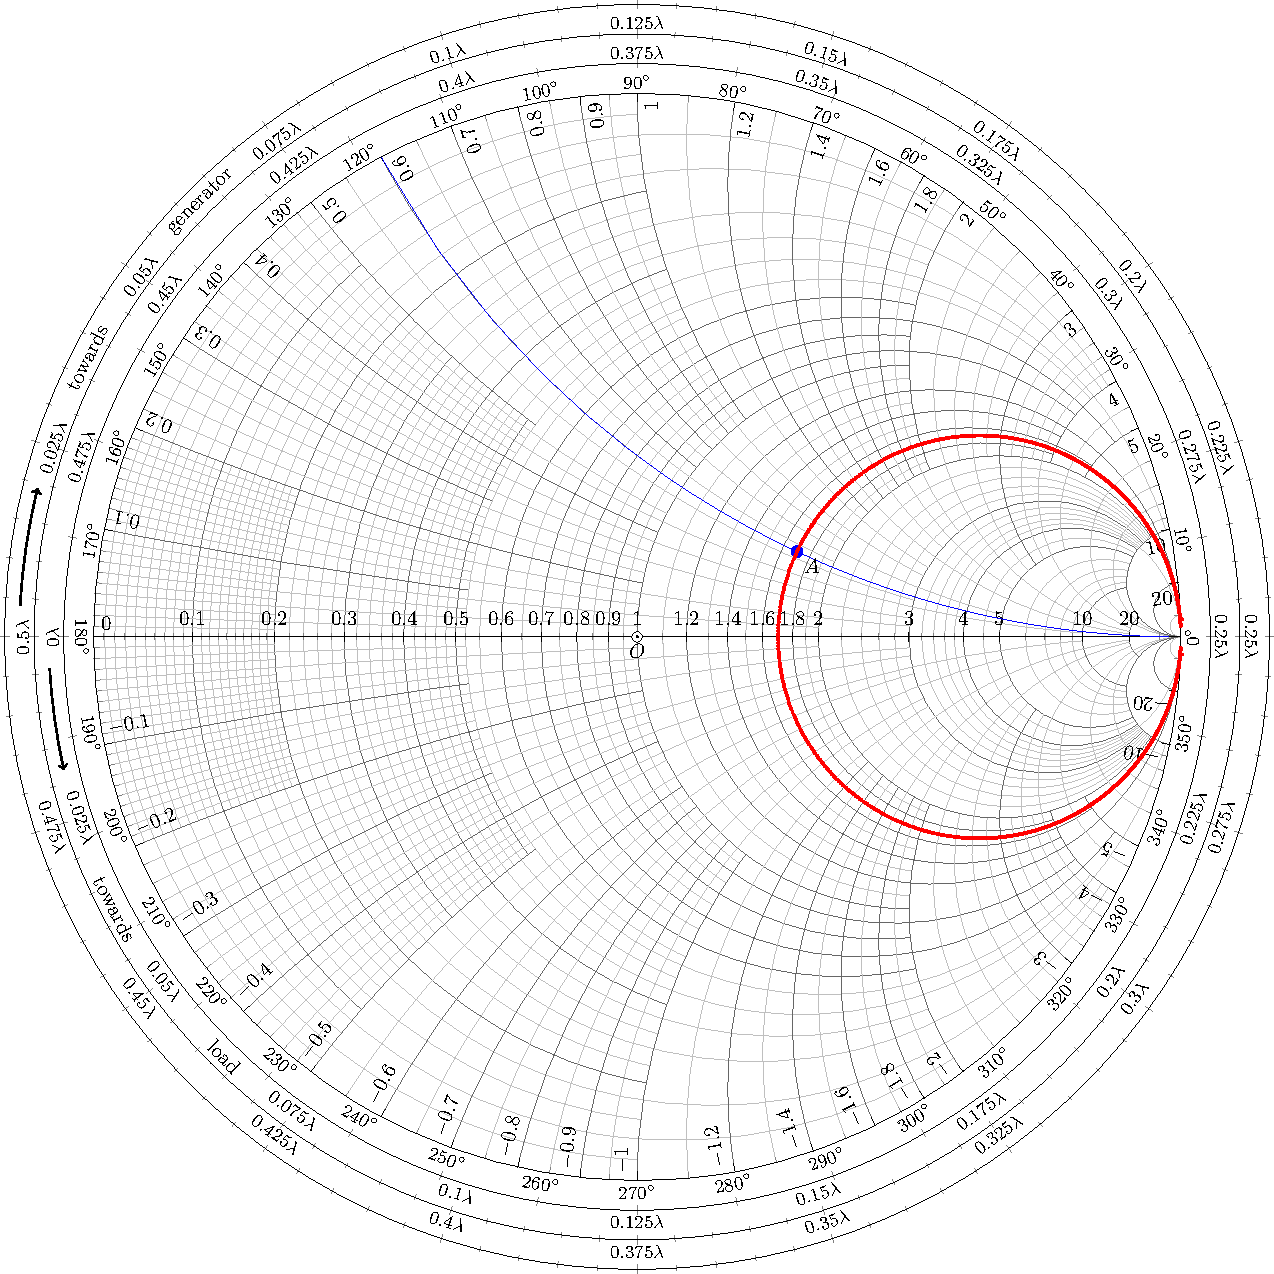
\includegraphics[width=7cm]{Cha4//fig4-12-3.pdf}}
      \only<4>{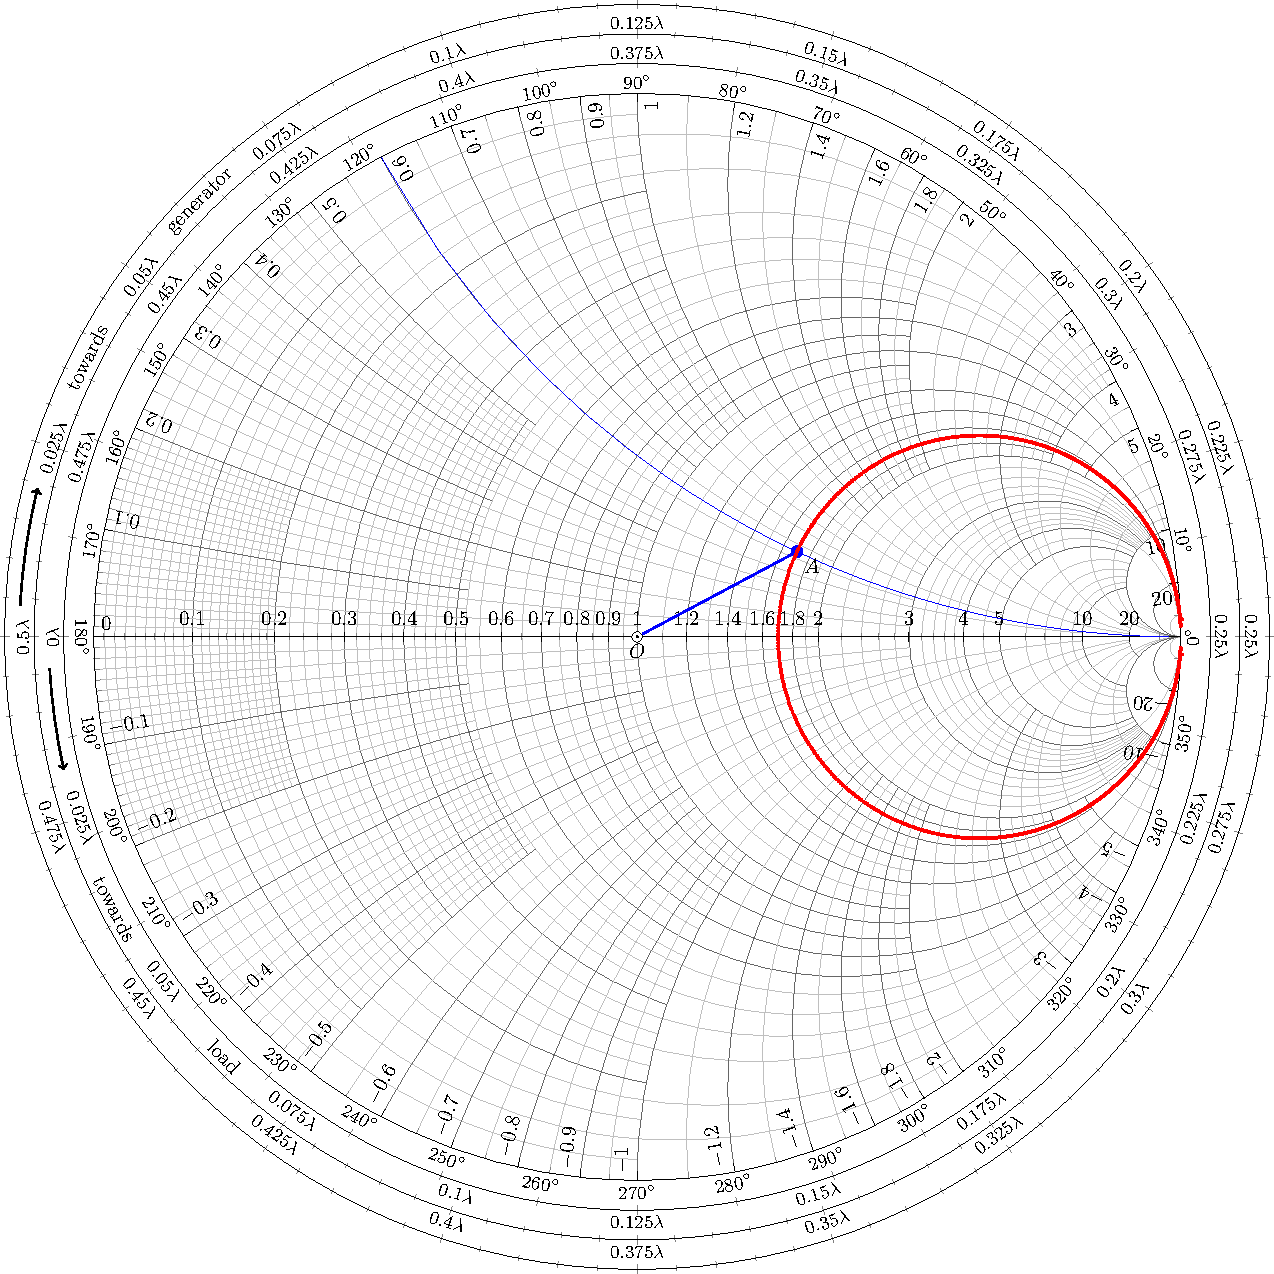
\includegraphics[width=7cm]{Cha4//fig4-12-4.pdf}}
      \only<5>{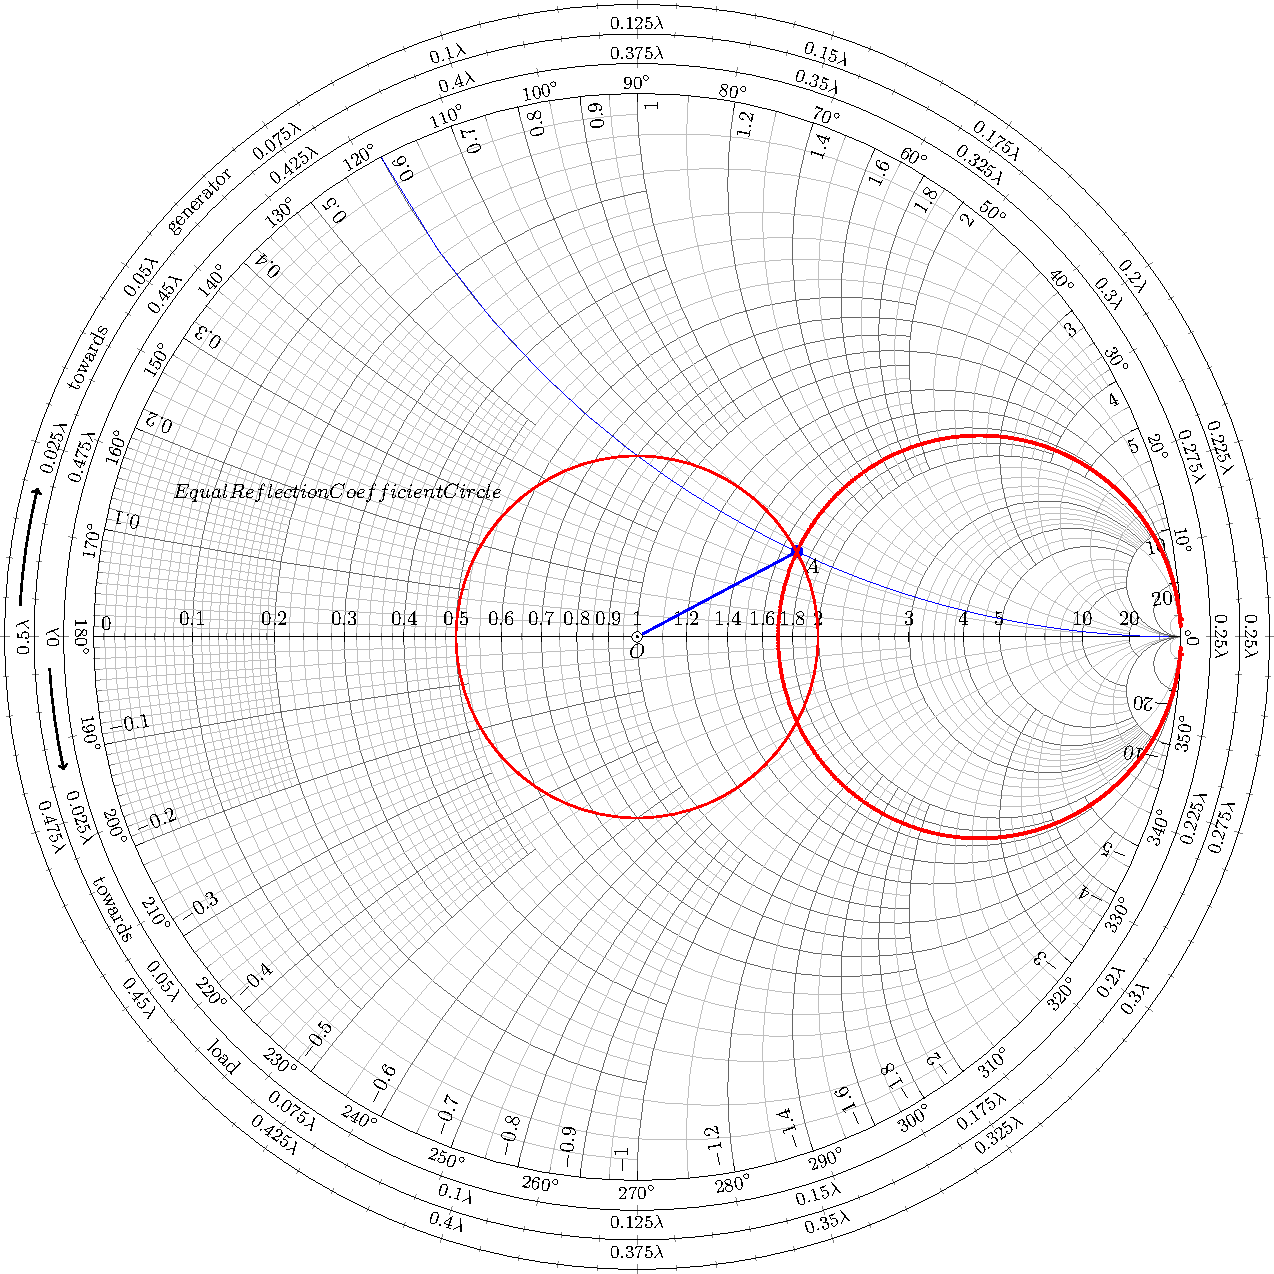
\includegraphics[width=7cm]{Cha4//fig4-12-5.pdf}}
      \only<6>{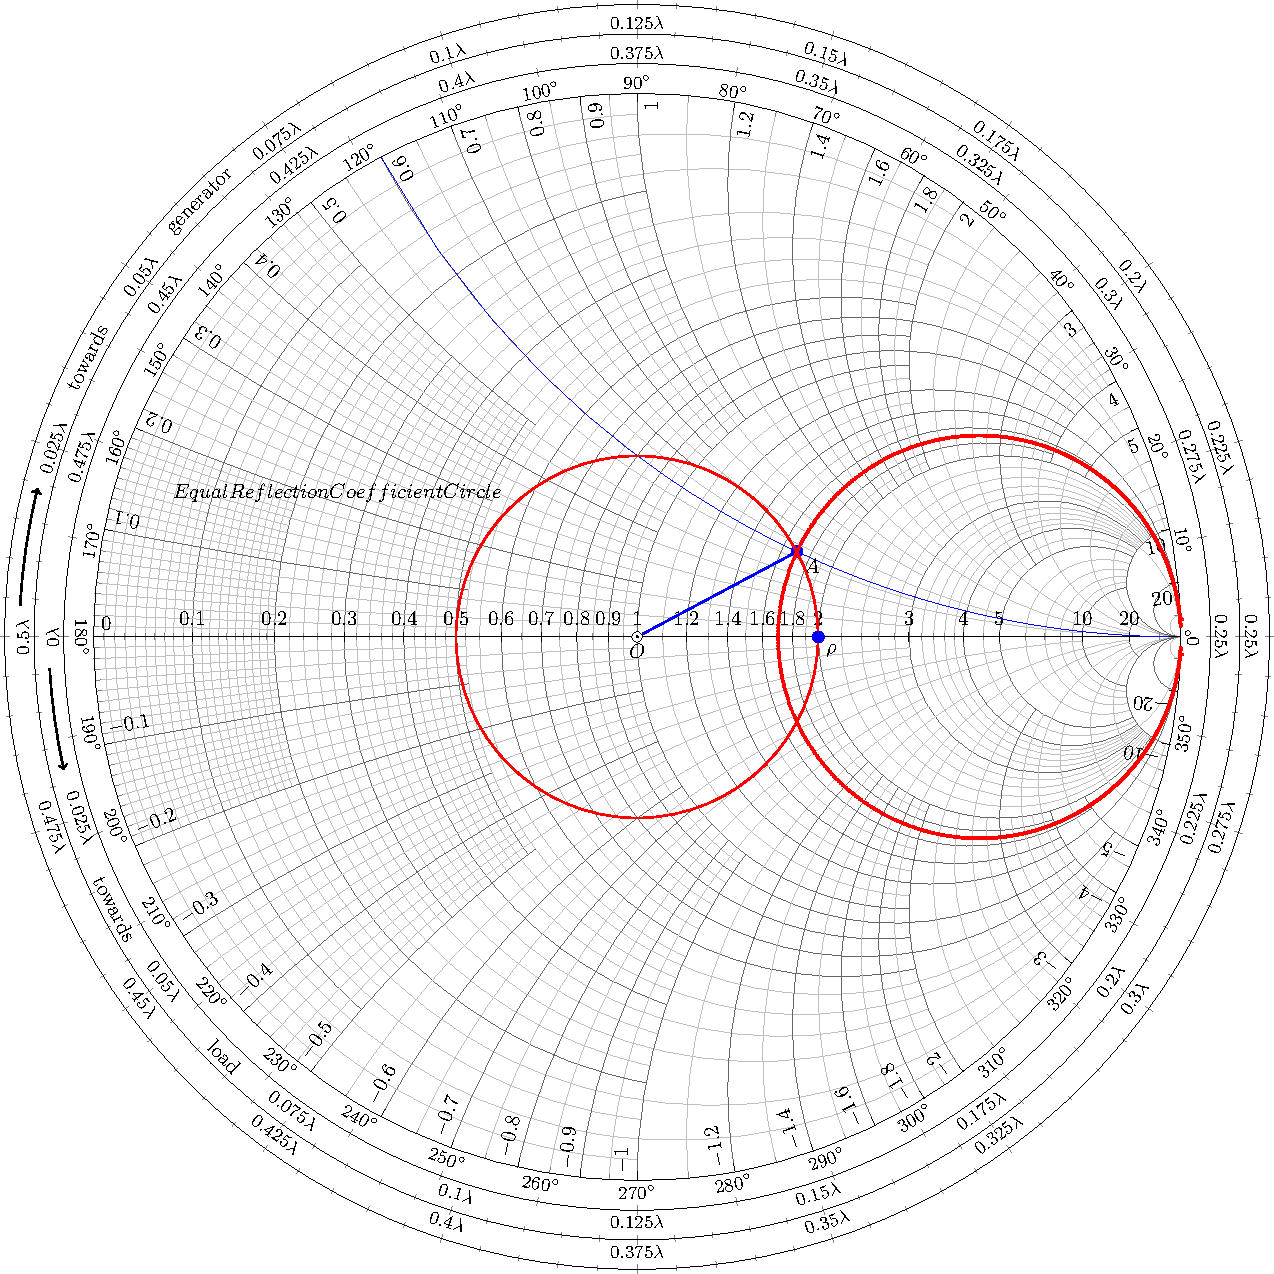
\includegraphics[width=7cm]{Cha4//fig4-12-6.pdf}}
      \only<7>{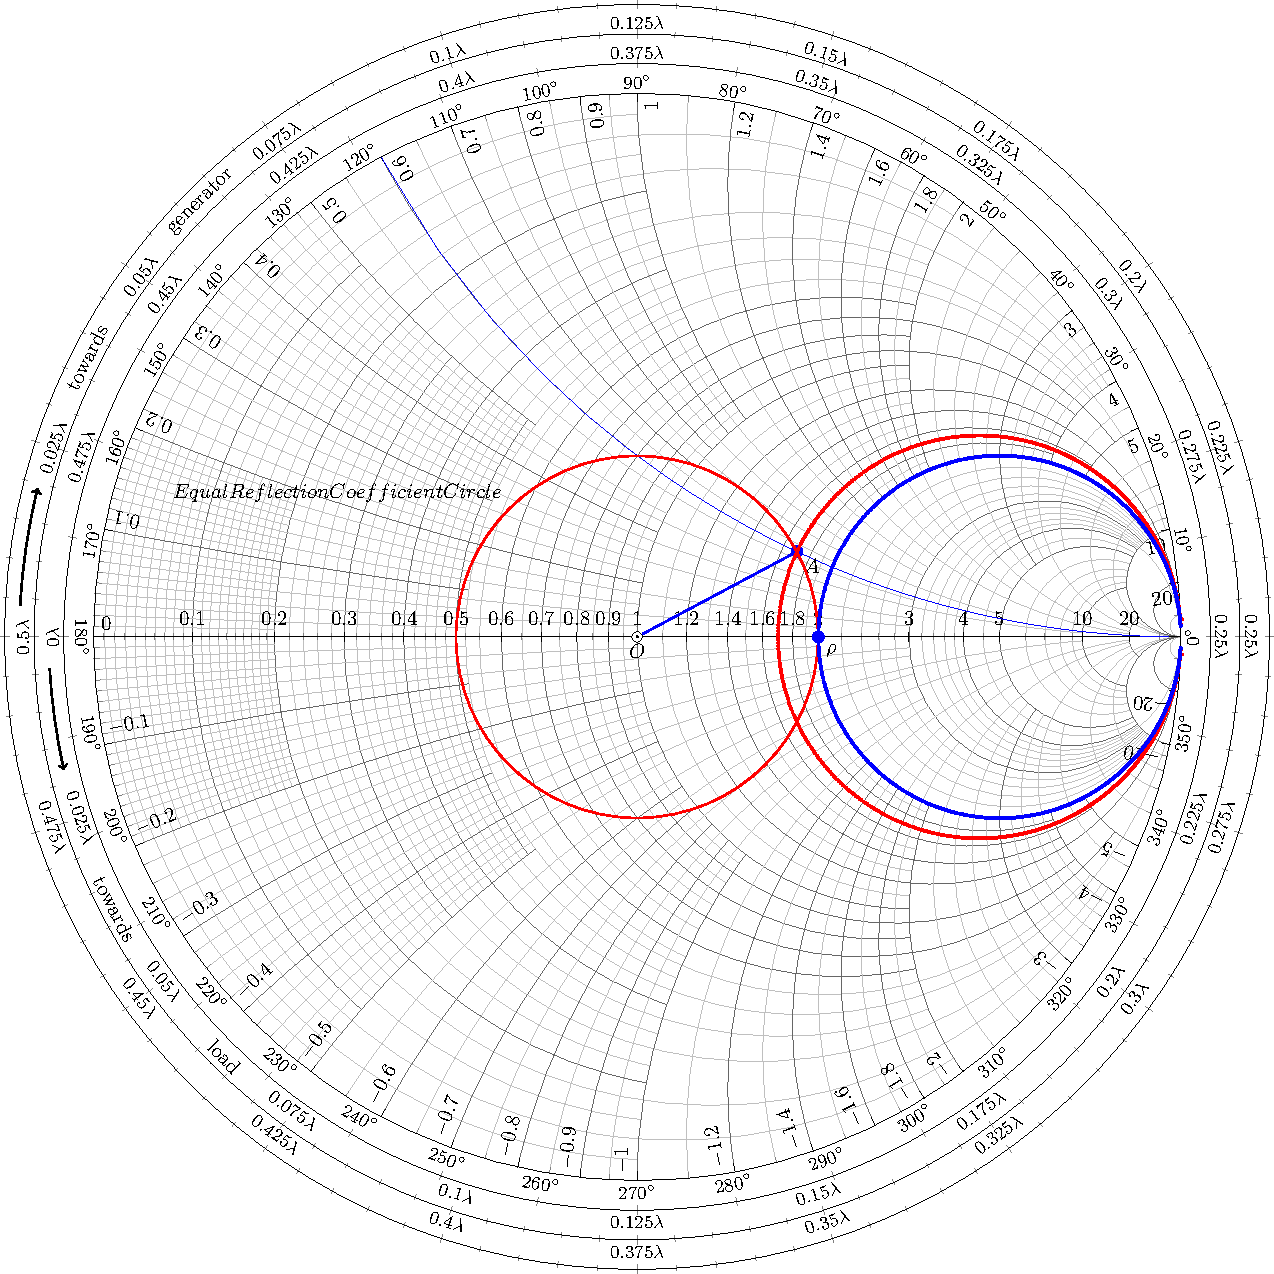
\includegraphics[width=7cm]{Cha4//fig4-12-7.pdf}}
    \end{column}
  \end{columns}
\end{frame}

\begin{frame}{Smith圆图的应用}
  例4 \quad 已知传输线长$l=25m$,特征阻抗为$100\Omega$,端接负载阻抗为$Z_L=(100-\mathrm{j}200)\Omega$,信号源频率为$f=10MHz$,利用Smith圆图求输入阻抗及导纳。
  \begin{columns}
    \begin{column}{0.4\linewidth}
      1)\quad 首先对负载归一化
      \begin{flalign*}
        z_L=\frac{Z_L}{Z_0}=1-\mathrm{j}2
      \end{flalign*}
      2)\quad 图中定位$A$点:$r=1,x=-2$,由题知$\lambda=30m$,传输线长$l=25m$,所以由$A$点沿等反射系数圆顺时针转动
      \begin{flalign*}
        \frac{l}{\lambda}=\frac{5}{6}=0.833=0.5+0.333
      \end{flalign*}
      到输入阻抗点,而
    \end{column}
    \begin{column}{0.6\linewidth}
      \only<1>{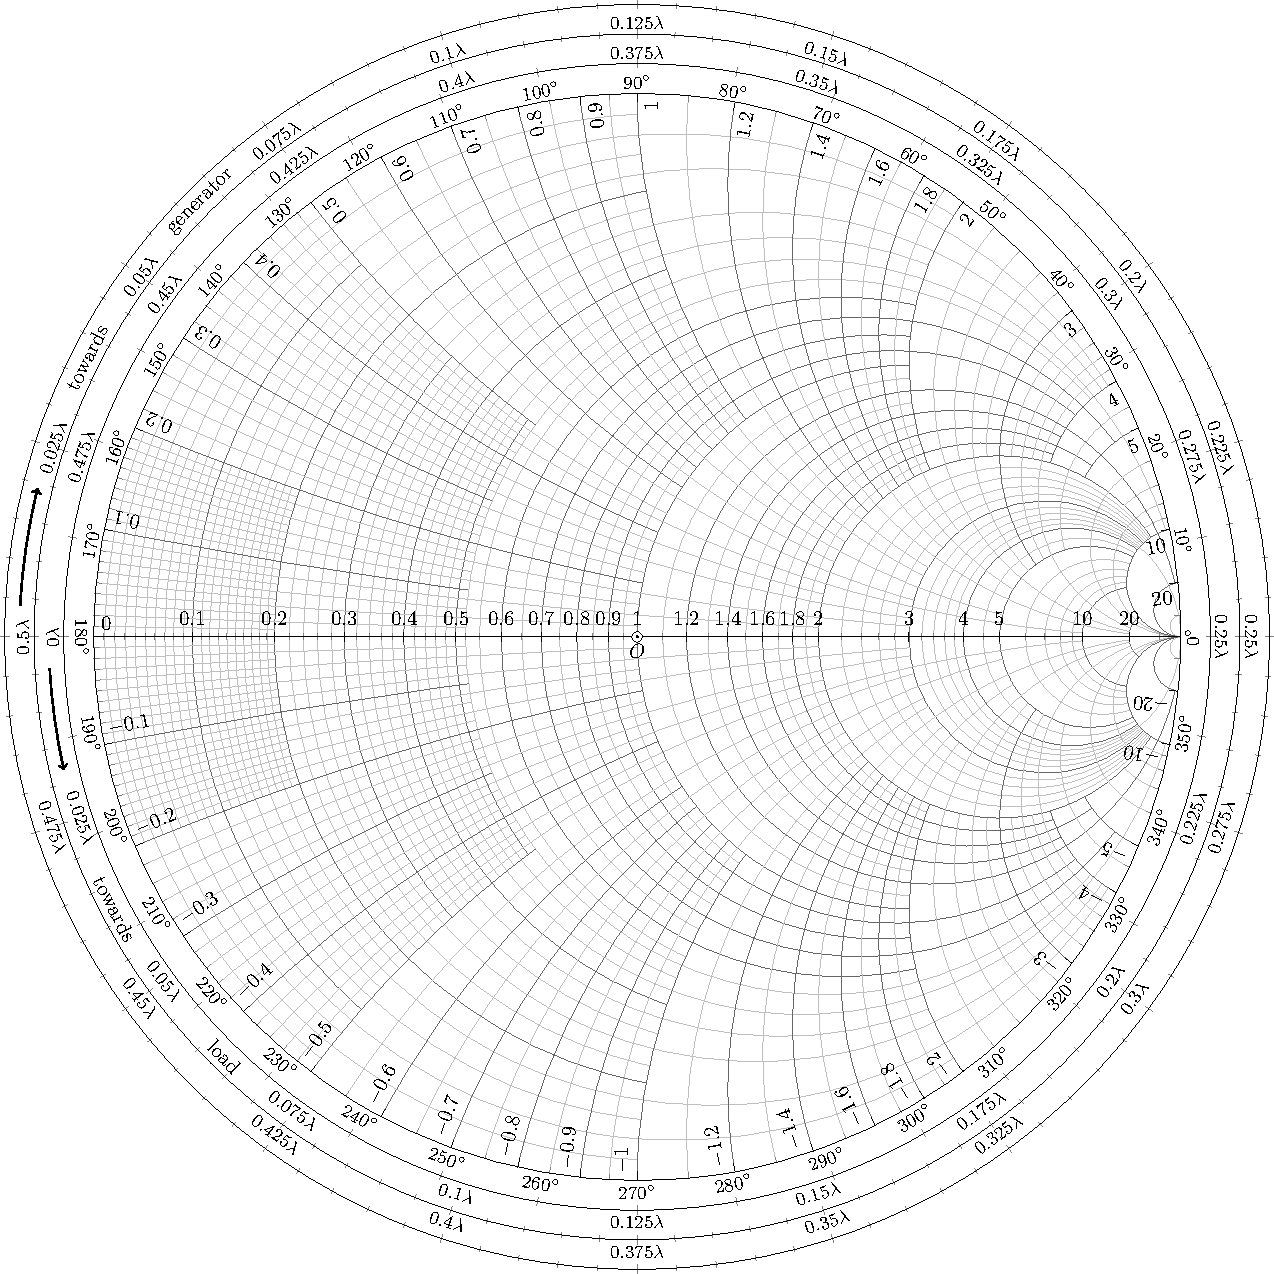
\includegraphics[width=6.5cm]{Cha4//fig4-13-1.pdf}}
      \only<2>{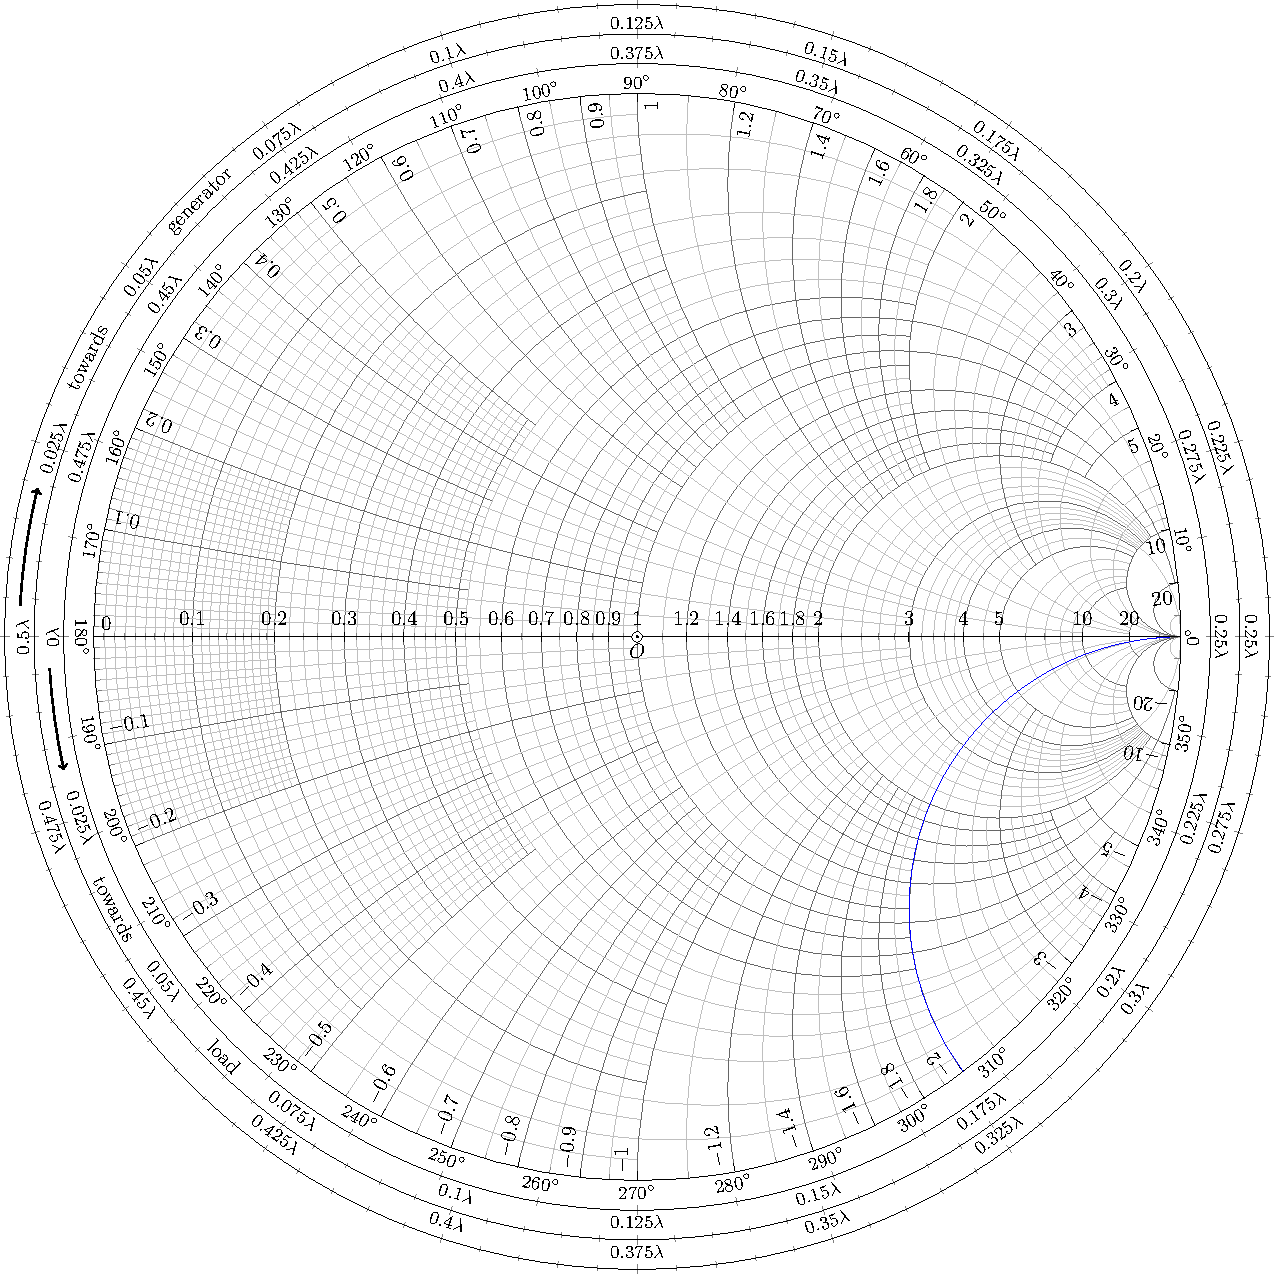
\includegraphics[width=6.5cm]{Cha4//fig4-13-2.pdf}}
      \only<3>{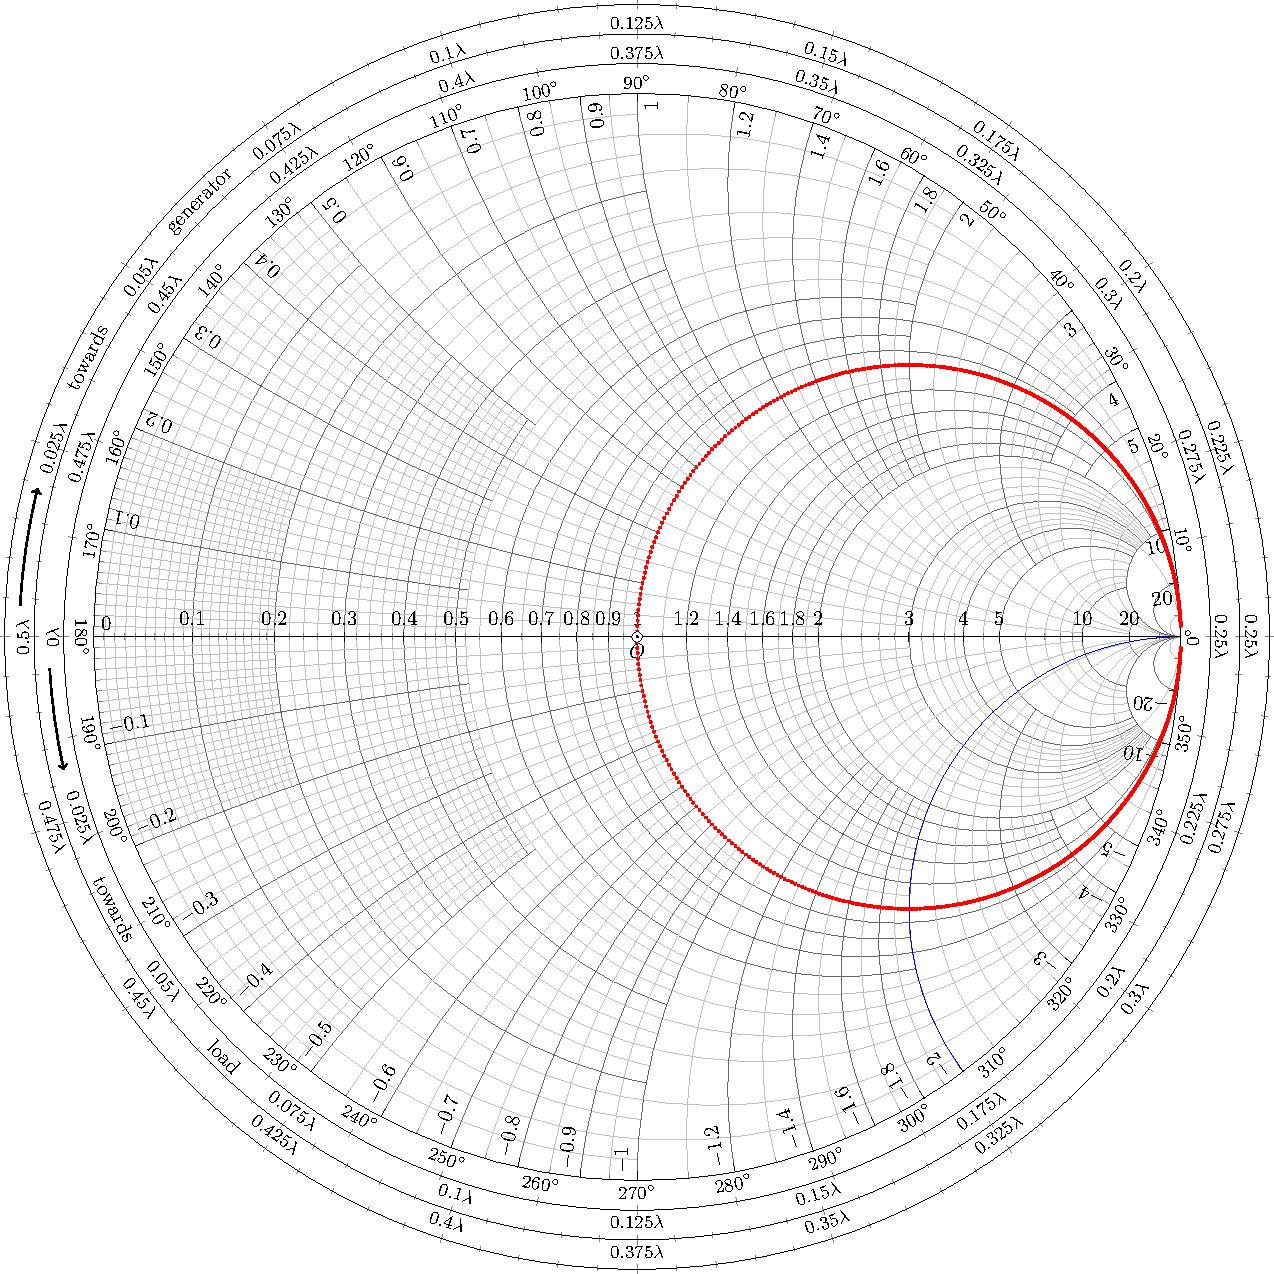
\includegraphics[width=6.5cm]{Cha4//fig4-13-3.pdf}}
      \only<4>{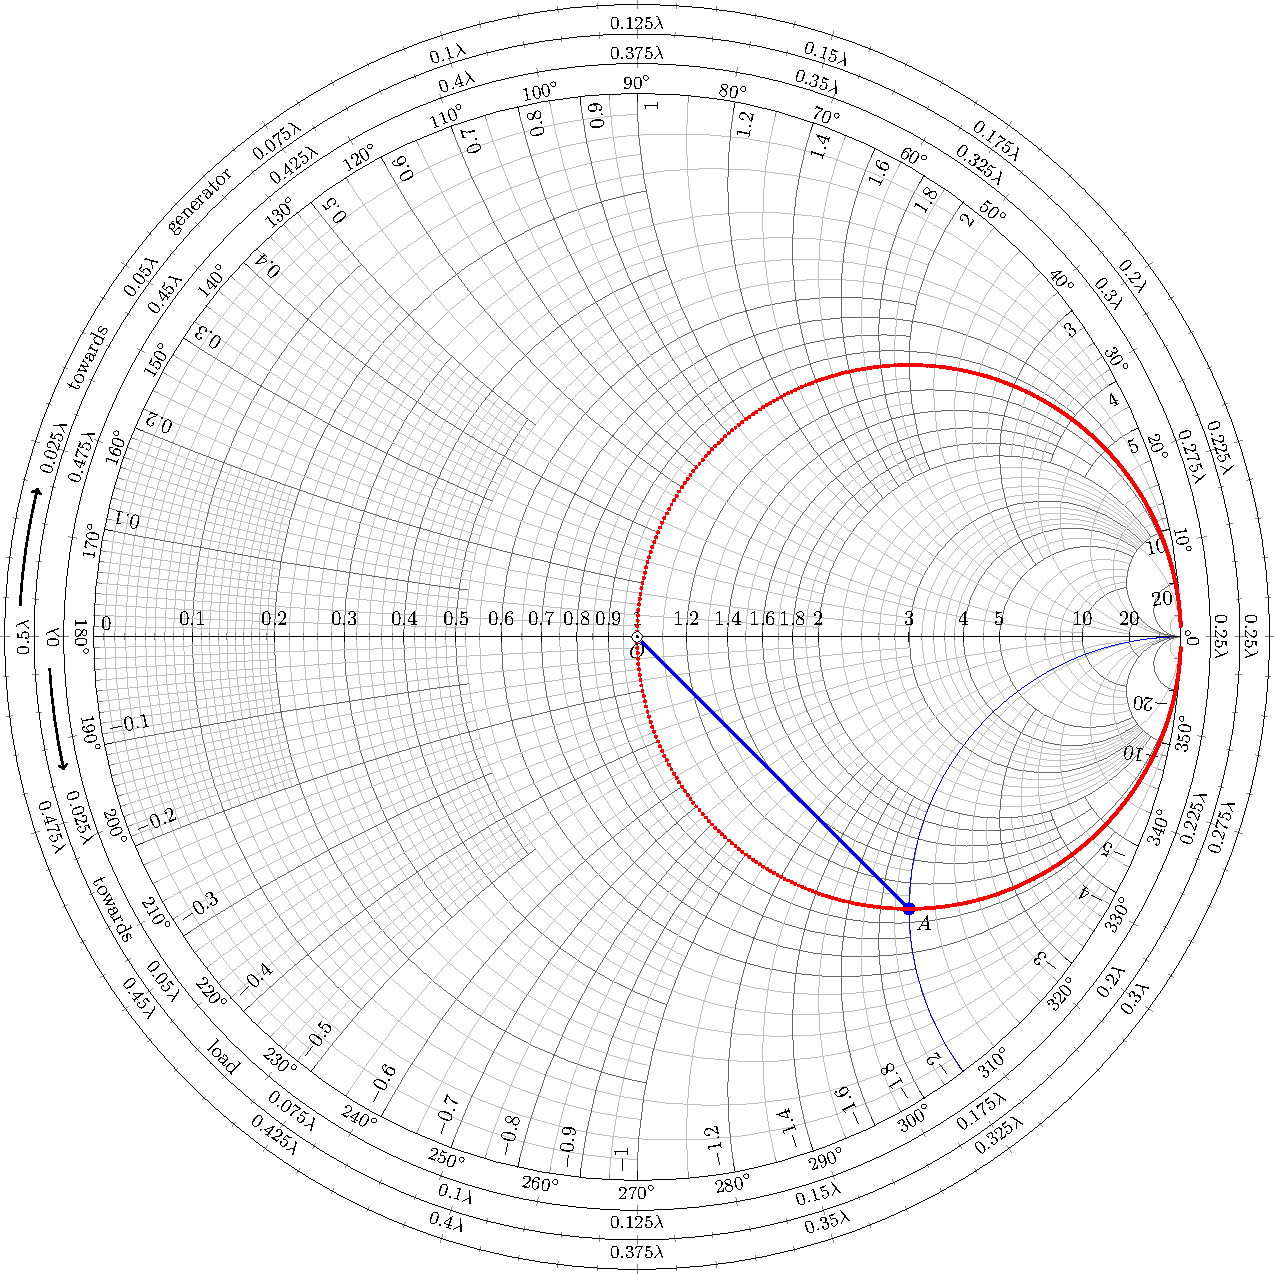
\includegraphics[width=6.5cm]{Cha4//fig4-13-4.pdf}}
      \only<5>{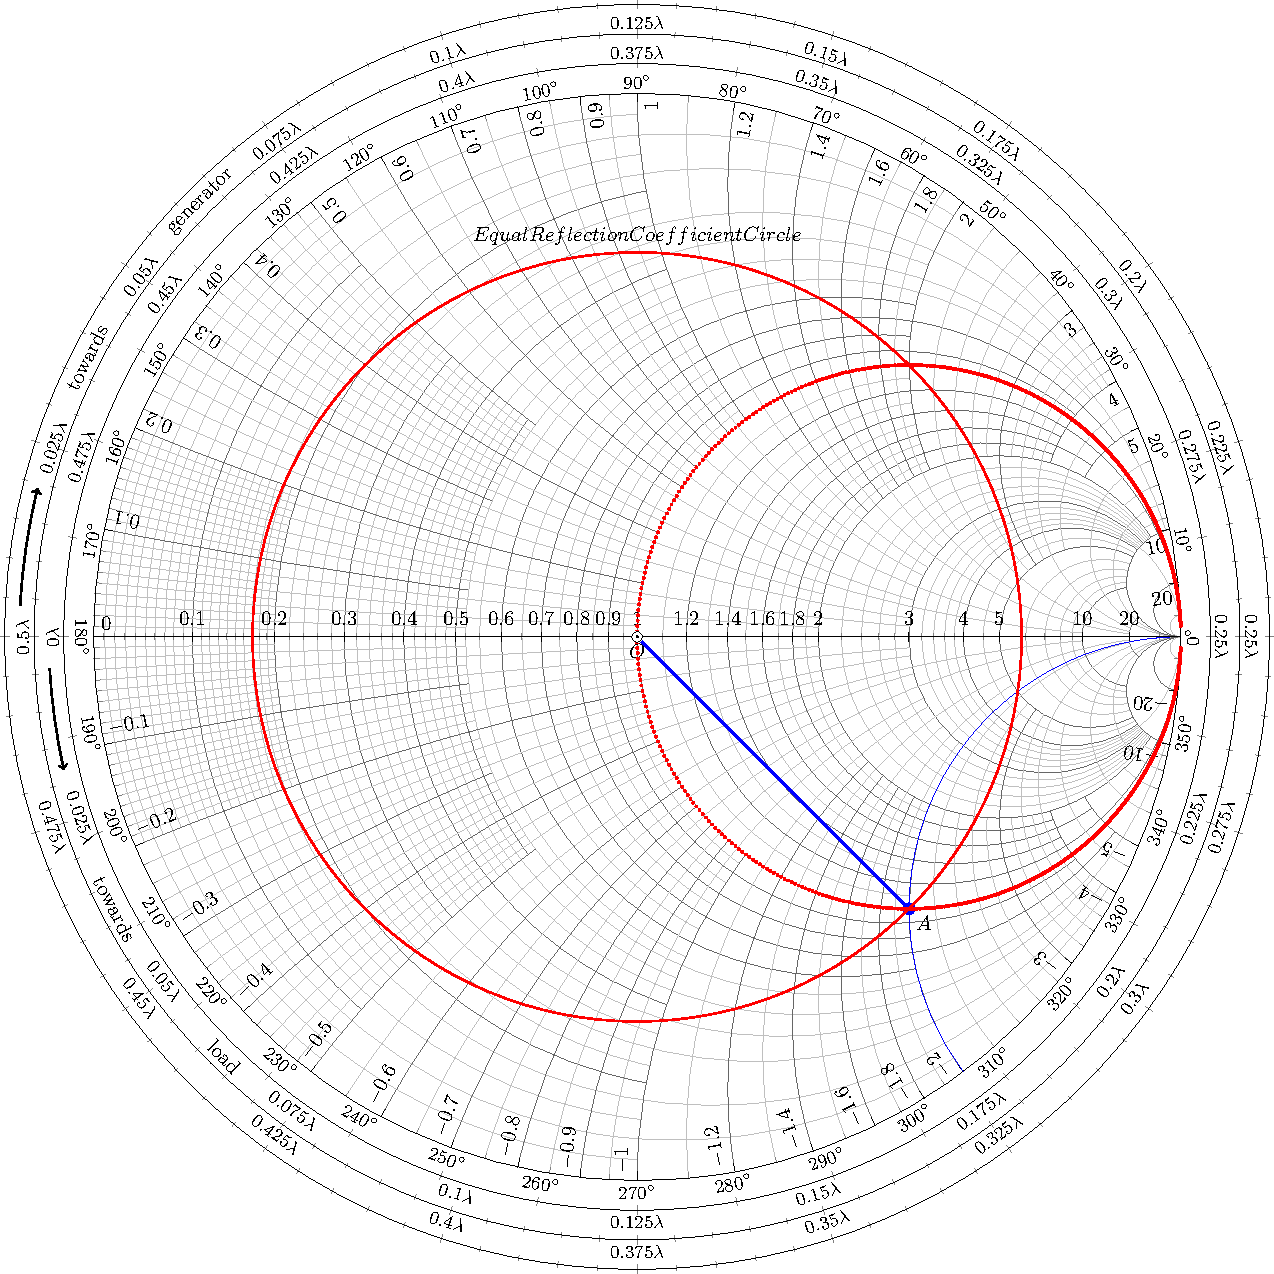
\includegraphics[width=6.5cm]{Cha4//fig4-13-5.pdf}}
    \end{column}
  \end{columns}
\end{frame}


\begin{frame}{Smith圆图的应用}
  \begin{columns}
    \begin{column}{0.4\linewidth}
      \begin{flalign*}
        2\beta l=4\pi\frac{5}{6}=2\pi+\frac{4}{3}\pi
      \end{flalign*}
      3)\quad 由负载对应的$A$点先沿等反射系数圆顺时针转动0.5刻度,对应$2\pi$,再转$\dfrac{4}{3}\pi$,对应0.333刻度,到达$B$点,$B$点即为输入阻抗点。从图中读出该点读数:$0.45+\mathrm{j}1.2$,反归一化,得到输入阻抗
      \begin{flalign*}
        Z_{in} & =(0.45+\mathrm{j}1.2)\times 100 \\
               & =(45+\mathrm{j}120)\Omega
      \end{flalign*}
    \end{column}
    \begin{column}{0.6\linewidth}
      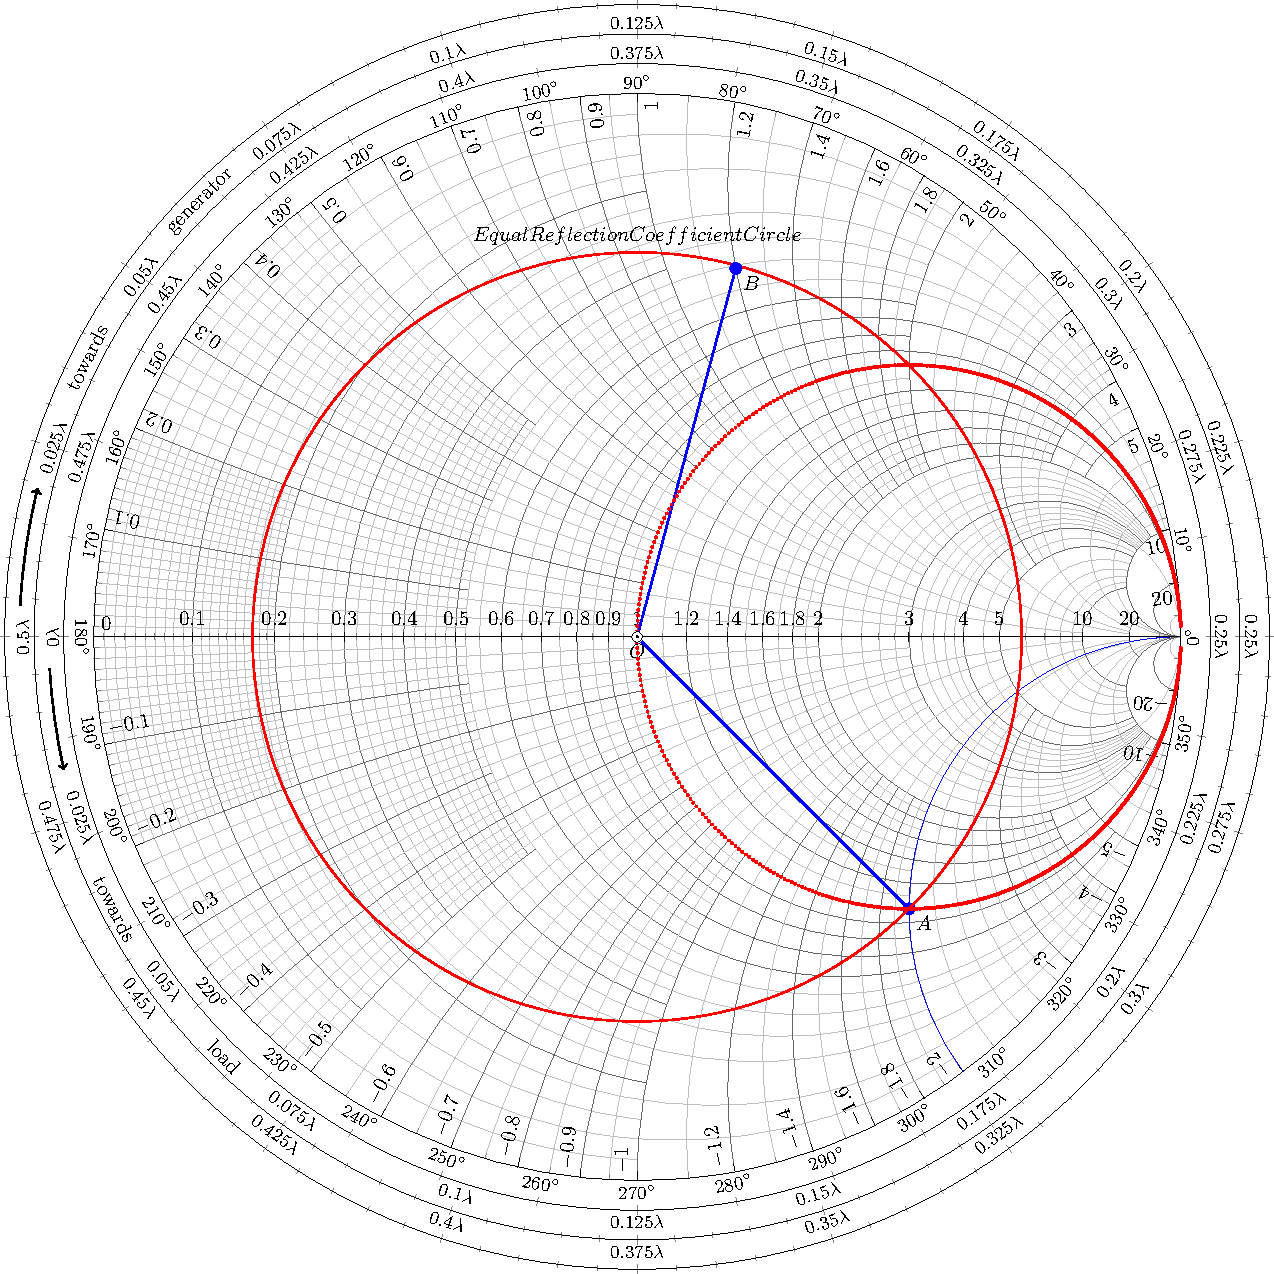
\includegraphics[width=6.5cm]{Cha4//fig4-13-6.pdf}
    \end{column}
  \end{columns}
\end{frame}

\begin{frame}{Smith圆图的应用}
  \begin{columns}
    \begin{column}{0.4\linewidth}
      4)\quad 再由$OB$反向延长到$C$点,为归一化导纳点,读出该点的值为$y_{in}=0.27-\mathrm{j}0.73$,所以输入导纳为
      \begin{flalign*}
        Y_{in} & =(0.27-\mathrm{j}0.73)/100 \\
               & =0.0027-\mathrm{j}0.0073
      \end{flalign*}
    \end{column}
    \begin{column}{0.6\linewidth}
      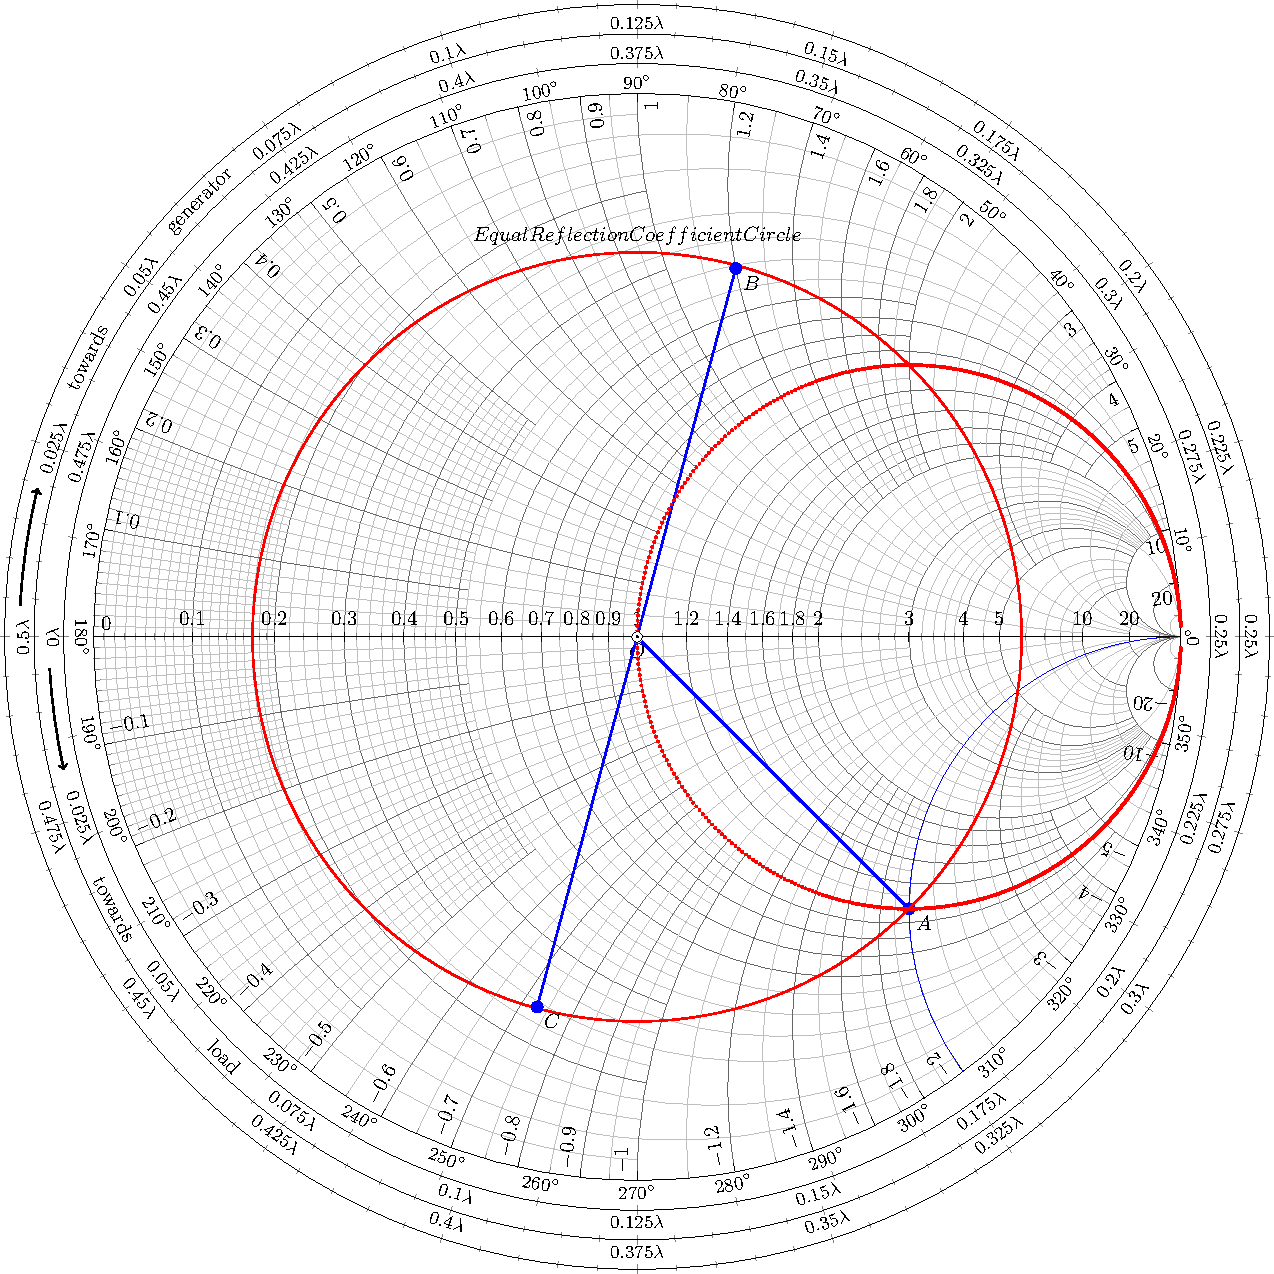
\includegraphics[width=6.5cm]{Cha4//fig4-13-7.pdf}
    \end{column}
  \end{columns}
\end{frame}

\begin{frame}{Smith圆图的应用}
  例5 \quad 如图所示,已知一无耗传输线的特性阻抗为$50\Omega$,驻波比$\rho=3$,相邻两个电压最小值点的距离为$0.2m$,距离负载最近的电压驻波最小值点距负载$0.05m$,求:(1)负载处反射系数;(2)负载阻抗
  \begin{columns}
    \begin{column}{0.4\linewidth}
      由题可知$\lambda/2=0.2m$,所以$\lambda=0.4m$,由已知条件有
      \begin{flalign*}
        \rho=\lvert V_{\mathrm{max}}\rvert / \lvert V_{\mathrm{min}}\rvert = 3
      \end{flalign*}
      因为$\rho=\dfrac{1+\lvert \Gamma \rvert}{1-\lvert \Gamma \rvert}$,所以
      \begin{flalign*}
        \lvert \Gamma_L \rvert = \lvert \Gamma \rvert = \frac{\rho-1}{\rho+1}=\frac{1}{2}
      \end{flalign*}
      1)\quad 绘出等反射系数圆

    \end{column}
    \begin{column}{0.6\linewidth}
      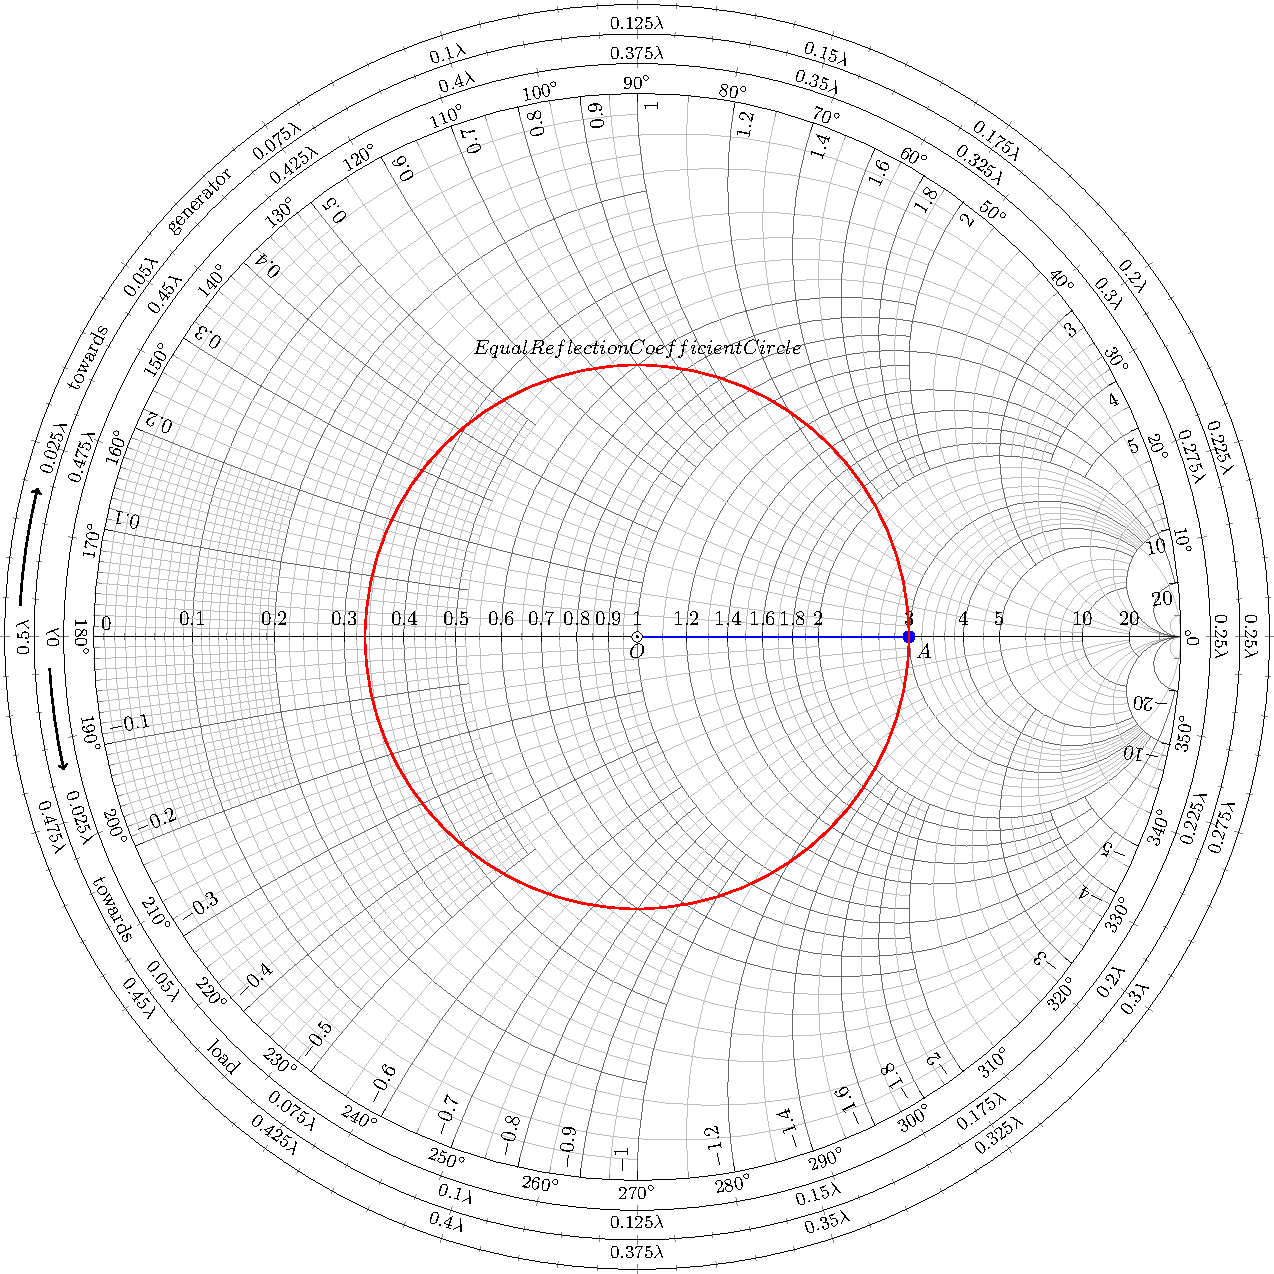
\includegraphics[width=6.5cm]{Cha4//fig4-16-1.pdf}
    \end{column}
  \end{columns}
\end{frame}

\begin{frame}{Smith圆图的应用}
  \begin{columns}
    \begin{column}{0.4\linewidth}
      2)\quad 第一个最小值点处反射波相位为$-\pi$,对应$E$点,延长$OE$,与单位圆交于点$H$,由$H$点向负载(逆时针)转动$\dfrac{d_{\mathrm{min}}}{\lambda}=\dfrac{1}{8}$刻度,得到点$F$。等反射系数圆与$OF$的交点
      为$G$点。由$G$点读出的即为归一化负载阻抗$0.6-\mathrm{j}0.8$,进行反归一化,得到负载阻抗为$(0.6-\mathrm{j}0.8)\times 50=30-\mathrm{j}40$\\
      3)\quad 由$G$点读出反射系数为:
      \begin{flalign*}
        \Gamma_L=-\mathrm{j}0.5
      \end{flalign*}
    \end{column}
    \begin{column}{0.6\linewidth}
      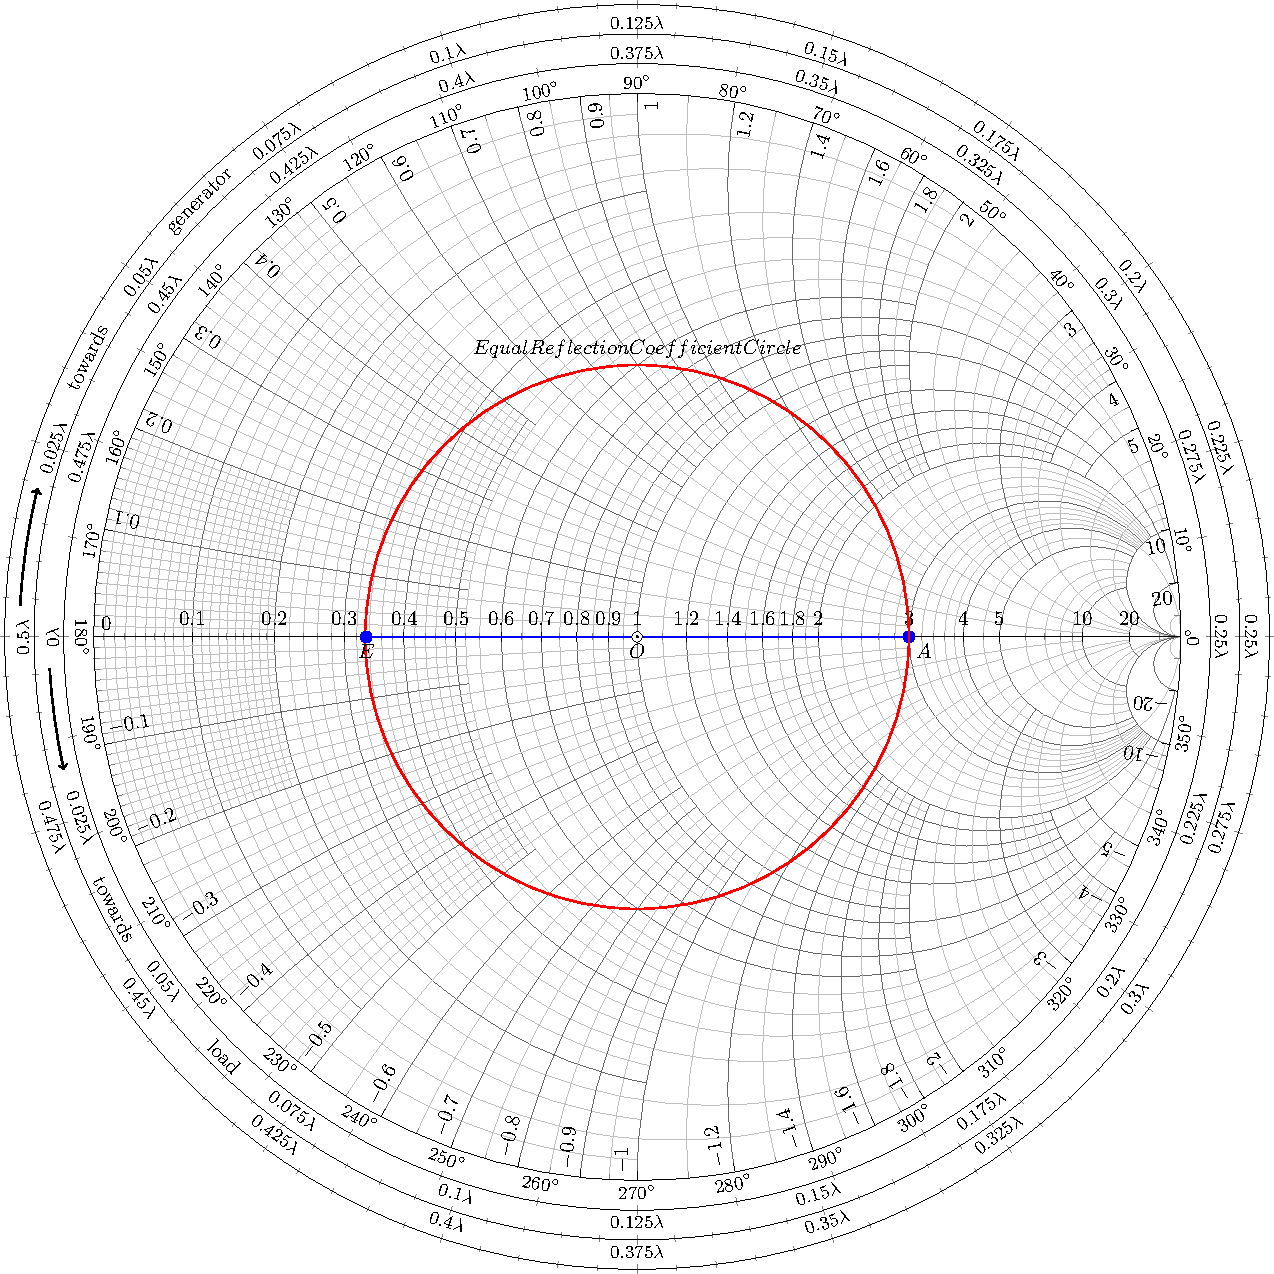
\includegraphics[width=6.5cm]{Cha4//fig4-16-2.pdf}
    \end{column}
  \end{columns}
\end{frame}

\begin{frame}{Smith圆图的应用}
  \begin{columns}
    \begin{column}{0.4\linewidth}
      2)\quad 第一个最小值点处反射波相位为$-\pi$,对应$E$点,延长$OE$,与单位圆交于点$H$,由$H$点向负载(逆时针)转动$\dfrac{d_{\mathrm{min}}}{\lambda}=\dfrac{1}{8}$刻度,得到点$F$。等反射系数圆与$OF$的交点
      为$G$点。由$G$点读出的即为归一化负载阻抗$0.6-\mathrm{j}0.8$,进行反归一化,得到负载阻抗为$(0.6-\mathrm{j}0.8)\times 50=30-\mathrm{j}40$\\
      3)\quad 由$G$点读出反射系数为:
      \begin{flalign*}
        \Gamma_L=-\mathrm{j}0.5
      \end{flalign*}
    \end{column}
    \begin{column}{0.6\linewidth}
      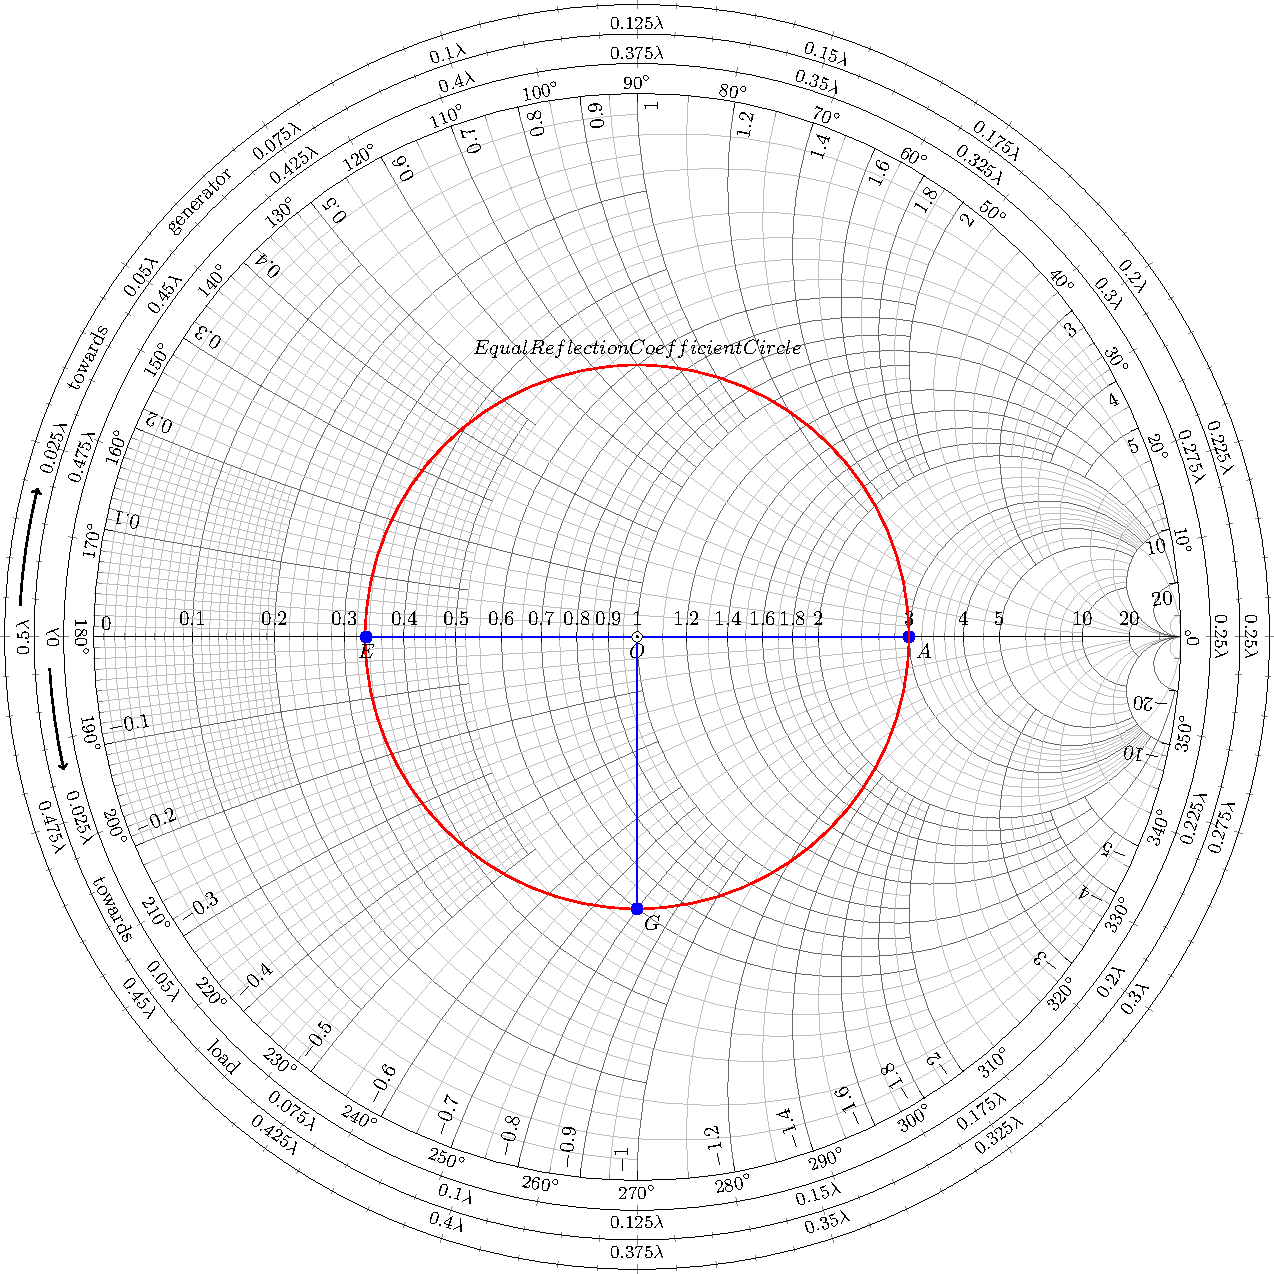
\includegraphics[width=6.5cm]{Cha4//fig4-16-3.pdf}
    \end{column}
  \end{columns}
\end{frame}

\begin{frame}{Smith圆图的应用}
  \begin{columns}
    \begin{column}{0.4\linewidth}
      2)\quad 第一个最小值点处反射波相位为$-\pi$,对应$E$点,延长$OE$,与单位圆交于点$H$,由$H$点向负载(逆时针)转动$\dfrac{d_{\mathrm{min}}}{\lambda}=\dfrac{1}{8}$刻度,得到点$F$。等反射系数圆与$OF$的交点
      为$G$点。由$G$点读出的即为归一化负载阻抗$0.6-\mathrm{j}0.8$,进行反归一化,得到负载阻抗为$(0.6-\mathrm{j}0.8)\times 50=30-\mathrm{j}40$\\
      3)\quad 由$G$点读出反射系数为:
      \begin{flalign*}
        \Gamma_L=-\mathrm{j}0.5
      \end{flalign*}
    \end{column}
    \begin{column}{0.6\linewidth}
      \includegraphics[width=6.5cm]{Cha4//fig4-16-4.pdf}
    \end{column}
  \end{columns}
\end{frame}

\begin{frame}{Smith圆图的应用}
  例6 \quad 已知一无耗传输线的特征阻抗为$50\Omega$,端接负载阻抗$Z_L$,驻波电压最大值和最小值分别为$V_{\mathrm{max}}=2.5V$和$V_{\mathrm{min}}=1V$,相邻两个电压最小值点距离为$0.05m$。当负载处由接纯电阻$R(R<Z_0)$
  改为接负载$Z_L$时,电压最小值向源方向移动$1.25cm$,求负载阻抗$Z_L$。
  \begin{columns}
    \begin{column}{0.4\linewidth}
      1)\quad 驻波比
      \begin{flalign*}
        \rho=\lvert V_{\mathrm{max}}\rvert/\lvert V_{\mathrm{min}}\rvert=2.5
      \end{flalign*}
      2)\quad 相邻两个电压最小值点的距离为0.05m,即半波长$\lambda/2=0.05m$,即$\lambda=0.1m$,从而移动$1.25cm$为$\lambda/8$。\\
      3)\quad 当负载处由纯电阻换为接负载$Z_L$时,电压最小值向源方向移动$\lambda/8$,相当于纯电阻点向源移动$\lambda/8$\\
    \end{column}
    \begin{column}{0.6\linewidth}
      \includegraphics[width=6cm]{Cha4//fig4-17-1.pdf}
    \end{column}
  \end{columns}
\end{frame}

\begin{frame}{Smith圆图的应用}
  \begin{columns}
    \begin{column}{0.4\linewidth}
      4)\quad 端接负载$Z_L$的传输系统的$A$点输入阻抗为$R$,由$\rho=2.5=r$可以确定等反射系数圆$\lvert\Gamma\rvert$\\
      5)\quad 由于端接纯电阻时对应电压最小值,$R$处电压最小,$r=R/Z_0<1$,说明纯电阻点在横轴的负半轴上$E$点,
    \end{column}
    \begin{column}{0.6\linewidth}
      \includegraphics[width=7cm]{Cha4//fig4-17-2.pdf}
    \end{column}
  \end{columns}
\end{frame}

\begin{frame}{Smith圆图的应用}
  \begin{columns}
    \begin{column}{0.4\linewidth}
      4)\quad 端接负载$Z_L$的传输系统的$A$点输入阻抗为$R$,由$\rho=2.5=r$可以确定等反射系数圆$\lvert\Gamma\rvert$\\
      5)\quad 由于端接纯电阻时对应电压最小值,$R$处电压最小,$r=R/Z_0<1$,说明纯电阻点在横轴的负半轴上$E$点,
    \end{column}
    \begin{column}{0.6\linewidth}
      \includegraphics[width=7cm]{Cha4//fig4-17-3.pdf}
    \end{column}
  \end{columns}
\end{frame}

\begin{frame}{Smith圆图的应用}
  \begin{columns}
    \begin{column}{0.4\linewidth}
      4)\quad 端接负载$Z_L$的传输系统的$A$点输入阻抗为$R$,由$\rho=2.5=r$可以确定等反射系数圆$\lvert\Gamma\rvert$\\
      5)\quad 由于端接纯电阻时对应电压最小值,$R$处电压最小,$r=R/Z_0<1$,说明纯电阻点在横轴的负半轴上$E$点,
    \end{column}
    \begin{column}{0.6\linewidth}
      \includegraphics[width=7cm]{Cha4//fig4-17-4.pdf}
    \end{column}
  \end{columns}
\end{frame}

\begin{frame}{Smith圆图的应用}
  \begin{columns}
    \begin{column}{0.4\linewidth}
      4)\quad 端接负载$Z_L$的传输系统的$A$点输入阻抗为$R$,由$\rho=2.5=r$可以确定等反射系数圆$\lvert\Gamma\rvert$\\
      5)\quad 由于端接纯电阻时对应电压最小值,$R$处电压最小,$r=R/Z_0<1$,说明纯电阻点在横轴的负半轴上$E$点,
    \end{column}
    \begin{column}{0.6\linewidth}
      \includegraphics[width=7cm]{Cha4//fig4-17-5.pdf}
    \end{column}
  \end{columns}
\end{frame}

\begin{frame}{Smith圆图的应用}
  \begin{columns}
    \begin{column}{0.4\linewidth}
      4)\quad 端接负载$Z_L$的传输系统的$A$点输入阻抗为$R$,由$\rho=2.5=r$可以确定等反射系数圆$\lvert\Gamma\rvert$\\
      5)\quad 由于端接纯电阻时对应电压最小值,$R$处电压最小,$r=R/Z_0<1$,说明纯电阻点在横轴的负半轴上$E$点,
    \end{column}
    \begin{column}{0.6\linewidth}
      \includegraphics[width=7cm]{Cha4//fig4-17-6.pdf}
    \end{column}
  \end{columns}
\end{frame}

\begin{frame}{Smith圆图的应用}
  \begin{columns}
    \begin{column}{0.4\linewidth}
      6)\quad 对于端接负载$Z_L$的传输系统,对应圆图上点$E$向负载逆时针旋转$\lambda/8$到点$G$,即得到$Z_L$。从圆图上读出归一化阻抗为
      $0.69-\mathrm{j}0.72$,所以负载阻抗为
      \begin{flalign*}
        Z_L & =0.69-\mathrm{j}0.72\times 50 \\
            & =(34.5-\mathrm{j}36)\Omega
      \end{flalign*}
      7)\quad 导纳为(对应F点)
      \begin{flalign*}
        Y_L=1/Z_L=0.02006\angle 46.23^{\circ} S
      \end{flalign*}
    \end{column}
    \begin{column}{0.6\linewidth}
      \includegraphics[width=7cm]{Cha4//fig4-17-7.pdf}
    \end{column}
  \end{columns}
\end{frame}

\begin{frame}{Smith圆图的应用}
  \begin{columns}
    \begin{column}{0.4\linewidth}
      6)\quad 对于端接负载$Z_L$的传输系统,对应圆图上点$E$向负载逆时针旋转$\lambda/8$到点$G$,即得到$Z_L$。从圆图上读出归一化阻抗为
      $0.69-\mathrm{j}0.72$,所以负载阻抗为
      \begin{flalign*}
        Z_L & =0.69-\mathrm{j}0.72\times 50 \\
            & =(34.5-\mathrm{j}36)\Omega
      \end{flalign*}
      7)\quad 导纳为(对应F点)
      \begin{flalign*}
        Y_L=1/Z_L=0.02006\angle 46.23^{\circ} S
      \end{flalign*}
    \end{column}
    \begin{column}{0.6\linewidth}
      \includegraphics[width=7cm]{Cha4//fig4-17-8.pdf}
    \end{column}
  \end{columns}
\end{frame}

\begin{frame}{Smith圆图的应用}
  \begin{columns}
    \begin{column}{0.4\linewidth}
      6)\quad 对于端接负载$Z_L$的传输系统,对应圆图上点$E$向负载逆时针旋转$\lambda/8$到点$G$,即得到$Z_L$。从圆图上读出归一化阻抗为
      $0.69-\mathrm{j}0.72$,所以负载阻抗为
      \begin{flalign*}
        Z_L & =0.69-\mathrm{j}0.72\times 50 \\
            & =(34.5-\mathrm{j}36)\Omega
      \end{flalign*}
      7)\quad 导纳为(对应F点)
      \begin{flalign*}
        Y_L=1/Z_L=0.02006\angle 46.23^{\circ} S
      \end{flalign*}
    \end{column}
    \begin{column}{0.6\linewidth}
      \includegraphics[width=7cm]{Cha4//fig4-17-9.pdf}
    \end{column}
  \end{columns}
\end{frame}

\begin{frame}{Smith圆图的应用}
  \begin{columns}
    \begin{column}{0.4\linewidth}
      6)\quad 对于端接负载$Z_L$的传输系统,对应圆图上点$E$向负载逆时针旋转$\lambda/8$到点$G$,即得到$Z_L$。从圆图上读出归一化阻抗为
      $0.69-\mathrm{j}0.72$,所以负载阻抗为
      \begin{flalign*}
        Z_L & =0.69-\mathrm{j}0.72\times 50 \\
            & =(34.5-\mathrm{j}36)\Omega
      \end{flalign*}
      7)\quad 导纳为(对应F点)
      \begin{flalign*}
        Y_L=1/Z_L=0.02006\angle 46.23^{\circ} S
      \end{flalign*}
    \end{column}
    \begin{column}{0.6\linewidth}
      \includegraphics[width=7cm]{Cha4//fig4-17-10.pdf}
    \end{column}
  \end{columns}
\end{frame}

\begin{frame}{Smith圆图的应用}
  \begin{columns}
    \begin{column}{0.4\linewidth}
      6)\quad 对于端接负载$Z_L$的传输系统,对应圆图上点$E$向负载逆时针旋转$\lambda/8$到点$G$,即得到$Z_L$。从圆图上读出归一化阻抗为
      $0.69-\mathrm{j}0.72$,所以负载阻抗为
      \begin{flalign*}
        Z_L & =0.69-\mathrm{j}0.72\times 50 \\
            & =(34.5-\mathrm{j}36)\Omega
      \end{flalign*}
      7)\quad 导纳为(对应F点)
      \begin{flalign*}
        Y_L=1/Z_L=0.02006\angle 46.23^{\circ} S
      \end{flalign*}
    \end{column}
    \begin{column}{0.6\linewidth}
      \includegraphics[width=7cm]{Cha4//fig4-17-11.pdf}
    \end{column}
  \end{columns}
\end{frame}

\begin{frame}{Smith导纳圆图}
  导纳情况:
  \begin{align*}
    y_L=\frac{1-\Gamma}{1+\Gamma}=\frac{1+\Gamma^{'}}{1-\Gamma^{'}} \quad \Gamma^{'}=-\Gamma
  \end{align*}
  令$y_L=g+\mathrm{j}b$,完全类似可导出电导圆方程
  \begin{align*}
    \left(\Gamma_r^{'}-\frac{g}{1+g}\right)^2+\Gamma_i^{'2}=\left(\frac{1}{1+g}\right)^2
  \end{align*}
  其中,圆心坐标是$(\frac{g}{1+g},0)$,半径为$\frac{1}{1+g}$。
  \begin{align*}
    \frac{g}{1+g}+\frac{1}{1+g}\equiv 1
  \end{align*}
  等电导圆与直线$\Gamma_r^{'}=1$相切。
\end{frame}

\begin{frame}{Smith导纳圆图}
  \begin{columns}
    \begin{column}{0.5\linewidth}
      \includegraphics[width=6cm]{Cha4//equal_G_circle1.png}
    \end{column}
    \begin{column}{0.5\linewidth}
      \includegraphics[width=6cm]{Cha4//equal_G_circle2.png}
    \end{column}
  \end{columns}
  
  
\end{frame}

\begin{frame}{Smith导纳圆图}
  同理,电纳圆方程为
  \begin{align*}
    (\Gamma_r^{'}-1)^2+\left(\Gamma_i^{'}-\frac{1}{b}\right)^2=\left(\frac{1}{b}\right)^2
  \end{align*}
  \begin{columns}
    \begin{column}{0.5\linewidth}
      \includegraphics[width=6cm]{Cha4//equal_B_circle1.png}
    \end{column}
    \begin{column}{0.5\linewidth}
      \includegraphics[width=6cm]{Cha4//equal_B_circle2.png}
    \end{column}
  \end{columns}

\end{frame}

\begin{frame}{Smith导纳圆图}
  在很多实际计算时,我们要用到导纳(特别是对于并联支节)。对比阻抗和导纳,在归一化情况下:
  \begin{align*}
    l=\frac{\lambda}{4} \quad Z_{in}=\lim_{\beta\cdot l\to \frac{\pi}{2}}\left(Z_0\cdot\frac{Z_L+\mathrm{j}Z_0\cdot\tan(\beta\cdot l)}{Z_0+\mathrm{j}Z_L\cdot\tan(\beta\cdot l)}\right)=Z_0^2\cdot\frac{1}{Z_L}
  \end{align*}
  非归一情况:$Y_L=\dfrac{Z_0^2}{Z_L}$ \\
  归一情况:$y_l=\dfrac{1}{z_l}$\\
  对应$\frac{\lambda_g}{4}$阻抗变换:$Z_{in}=\dfrac{1}{z_l}$
\end{frame}

\begin{frame}{Smith导纳圆图}
  \begin{itemize}
    \item 导纳圆图
  \end{itemize}
  \centering
  \begin{table}
    \caption{阻抗原图与导纳圆图对应关系}
    \begin{tabular}{|c|c|}
      \hline
      \textbf{阻抗圆图} & \textbf{导纳圆图} \\ \hline
      $r$           & $g$           \\ \hline
      $x$           & $b$           \\ \hline
      $\Gamma(z)$   & $\Gamma_I(z)$ \\ \hline
      电压振幅值腹点       & 电流振幅值腹点       \\ \hline
      电压振幅值节点       & 电流振幅值节点       \\ \hline
      开路点           & 短路点           \\ \hline
      短路点           & 开路点           \\
      \hline
    \end{tabular}
  \end{table}
\end{frame}

\begin{frame}{Smith导纳圆图}
  例7 \quad 负载$Z_L=100+\mathrm{j}50\Omega$,端接$50\Omega$传输线,传输线长$0.15\lambda$,用Smith圆图求解负载导纳及输入导纳。
  \begin{columns}
    \begin{column}{0.4\linewidth}

      1)\quad 负载归一化:
      \begin{flalign*}
        z_L=\frac{Z_L}{Z_0}=2+\mathrm{j}1
      \end{flalign*}

      2)\quad 利用Smith阻抗圆图,定位A点,旋转$180^{\circ}$,得B点,阻抗圆图中读出的是归一化阻抗数值,这个数值即为负载归一化导纳:
      \begin{flalign*}
        y_L=0.4-\mathrm{j}0.2=\frac{1}{2+\mathrm{j}1}=\frac{1}{z_L}
      \end{flalign*}

    \end{column}
    \begin{column}{0.6\linewidth}
      \only<1>{\includegraphics[width=7cm]{Cha4//fig4-22-1.pdf}}
      \only<2>{\includegraphics[width=7cm]{Cha4//fig4-22-2.pdf}}
      \only<3>{\includegraphics[width=7cm]{Cha4//fig4-22-3.pdf}}
      \only<4>{\includegraphics[width=7cm]{Cha4//fig4-22-4.pdf}}
      \only<5>{\includegraphics[width=7cm]{Cha4//fig4-22-5.pdf}}
      \only<6>{\includegraphics[width=7cm]{Cha4//fig4-22-6.pdf}}
      \only<7>{\includegraphics[width=7cm]{Cha4//fig4-22-7.pdf}}
    \end{column}
  \end{columns}
\end{frame}

\begin{frame}{Smith导纳圆图}
  \begin{columns}
    \begin{column}{0.4\linewidth}
      3)\quad 用导纳圆图求归一化输入导纳(反射系数为电流反射系数,形状读数不变),在导纳圆图中找到负载归一化导纳点$y_L=0.4-\mathrm{j}0.2$,顺时针旋转$0.15\lambda$,得归一化输入导纳$y_{in}=0.61+\mathrm{j}0.66$,
      反归一化得到输入导纳
      \begin{flalign*}
        Y_{in} & =y_{in}/Z_0                \\
               & =(0.61+\mathrm{j}0.66)/50  \\
               & =0.0122+\mathrm{j}0.0132 S
      \end{flalign*}
    \end{column}
    \begin{column}{0.6\linewidth}
      \only<1>{\includegraphics[width=7cm]{Cha4//fig4-22-8.pdf}}
    \end{column}
  \end{columns}
\end{frame}

\subsection{阻抗匹配}
\begin{frame}{阻抗匹配}
  \begin{flalign*}
     & Z_{in}=R_{in}+\mathrm{j}X_{in}=Z_0\cdot \frac{Z_L+\mathrm{j}Z_0\cdot\tan (\beta l)}{Z_0+\mathrm{j}Z_L\cdot\tan (\beta l)}                                                                                           \\
     & P =\frac{1}{2}Re(V_{in}I_{in}^*)=\frac{1}{2}\lvert V_{in}\rvert^2Re\left(\frac{1}{Z_{in}}\right)=\frac{1}{2}\lvert V_{S}\rvert^2 \left\lvert\frac{Z_{in}}{Z_{in}+Z_S}\right\rvert^2 Re\left(\frac{1}{Z_{in}}\right)
  \end{flalign*}
  令$Z_S=R_S+\mathrm{j}X_S,Z_{in}=R_{in}+\mathrm{j}X_{in}$
  上式简化为
  \begin{flalign*}
    \color{blue}{P=\frac{1}{2}\lvert V_S\rvert^2\frac{R_{in}}{(R_{in}+R_{S})^2+(X_{in}+X_S)^2}} &  &
  \end{flalign*}

  \begin{figure}
    \flushright
    \includegraphics[width=6cm]{Cha4//fig4-24.pdf}
  \end{figure}
\end{frame}

\begin{frame}{阻抗匹配}
  \begin{enumerate}
    \item 负载与传输线匹配$Z_L=Z_0$
          \saveenum
  \end{enumerate}
  \begin{align*}
    \Gamma_L=\frac{Z_L-Z_0}{Z_L+Z_0}=0 \quad Z_{in}=Z_0\cdot \frac{Z_L+\mathrm{j}Z_0\cdot \tan(\beta l)}{Z_0+\mathrm{j}Z_L\cdot \tan(\beta l)}=Z_0
  \end{align*}
  传递至负载的功率为
  \begin{align*}
    P_{L1}=\frac{1}{2}\lvert V_S \rvert^2\frac{Z_0}{(Z_0+R_S)^2+X_S^2}
  \end{align*}

  \begin{flalign*}
    \color{blue}{P=\frac{1}{2}\lvert V_S\rvert^2\frac{R_{in}}{(R_{in}+R_{S})^2+(X_{in}+X_S)^2}} &  &
  \end{flalign*}
  \begin{figure}
    \flushright
    \includegraphics[width=5.5cm]{Cha4//fig4-24.pdf}
  \end{figure}
\end{frame}

\begin{frame}{阻抗匹配}
  \begin{enumerate}
    \resume
    \item 源与带载传输线匹配$Z_S=Z_{in}$
          \saveenum
  \end{enumerate}
  \begin{align*}
    \Gamma_{in}=\frac{Z_{in}-Z_S}{Z_{in}+Z_S}=0
  \end{align*}
  传递至负载的功率为
  \begin{align*}
    P_{L2}=\frac{1}{2}\lvert V_S \rvert^2\frac{R_S}{4(R_S^2+X_S^2)}
  \end{align*}

  \begin{flalign*}
    \color{blue}{P=\frac{1}{2}\lvert V_S\rvert^2\frac{R_{in}}{(R_{in}+R_{S})^2+(X_{in}+X_S)^2}} &  &
  \end{flalign*}
  \begin{figure}
    \flushright
    \includegraphics[width=5.5cm]{Cha4//fig4-24.pdf}
  \end{figure}
\end{frame}

\begin{frame}{阻抗匹配}
  \begin{enumerate}
    \resume
    \item 共轭匹配
  \end{enumerate}
  $$\color{blue}{P=\frac{1}{2}\lvert V_S\rvert^2\frac{R_{in}}{(R_{in}+R_{S})^2+(X_{in}+X_S)^2}}$$
  \begin{align*}
     & \frac{\partial P}{\partial R_{in}}=0 \quad \Longrightarrow                                               \\
     & \frac{1}{(R_{in}+R_S)^2+(X_{in}+X_S)^2}+\frac{-2R_{in}(R_{in}+R_S)}{[(R_{in}+R_S)^2+(X_{in}+X_S)^2]^2}=0 \\
     & R_S^2-R_{in}^2+(X_{in}+X_S)^2=0                                                                          \\
    \\
     & \frac{\partial P}{\partial X_{in}}=0 \quad \Longrightarrow                                               \\
     & \frac{-2R_{in}(X_{in}+X_S)}{[(R_{in}+R_S)^2+(X_{in}+X_S)^2]^2}=0                                         \\
     & X_{in}(X_{in}+X_S)=0
  \end{align*}
\end{frame}

\begin{frame}{阻抗匹配}
  \begin{align*}
    R_S=R_{in} \quad X_S=-X_{in}
  \end{align*}
  $$\downarrow$$
  \begin{empheq}[box=\widefbox]{align*}
    Z_{in} = Z_S^*
  \end{empheq}
  传递至负载的功率:
  \begin{align*}
    P_{L3}=\frac{1}{2}\lvert V_S\rvert^2\frac{1}{4R_S} \\
    P_{L3}\geqslant P_{L1},P_{L3}\geqslant P_{L2}
  \end{align*}
  若源阻抗为实数 $P_{L3}=P_{L2}$
\end{frame}

\begin{frame}{阻抗匹配}
  \begin{itemize}
    \item 匹配的意义
          \begin{itemize}
            \item 传输线的功率容量最大\\
                  行波状态时传输线的功率容量最大,因为不匹配时的驻波场,在波腹处的电场比传输同样功率的行波电场大得多,故而容易发生击穿,使功率容量降低
            \item 微波源工作稳定\\
                  行波状态时,对信号源无影响,使微波源工作稳定
          \end{itemize}
    \item 匹配器
          \begin{itemize}
            \item 人为引入新的不均匀性以造成新的反射去抵消(或大大削弱)失配所引起的反射
            \item 匹配器的主要目的是为了使负载能得到最大功率,故匹配器本身不能有损耗,它应由\uline{纯无功元件}构成
            \item 理想的匹配,反射系数为0;实际工程中,在指定的频率范围内反射系数小于规定的值
            \item 阻抗匹配器类型 \\
                  窄带,宽带\\
                  支节匹配器:单支节、双支节\\
                  四分之一波长阻抗变换器,渐变变换器\\
                  ……
          \end{itemize}
  \end{itemize}
\end{frame}

\subsection{支节匹配器}
\begin{frame}{支节匹配器}
  \begin{itemize}
    \item 并联单支节匹配
  \end{itemize}
  \centering
  \begin{figure}
    \includegraphics[width=12cm]{Cha4//fig4-23.pdf}
  \end{figure}
\end{frame}

\begin{frame}{支节匹配器}
  $$Y_A=Y_{stub}+Y(d_{stub})=Y_0=\frac{1}{Z_0}$$
  \begin{columns}
    \begin{column}{0.5\linewidth}
      $Y_{stub}$:支节线引入的输入导纳\\
      \includegraphics[width=5cm]{Cha4//fig4-25.pdf}
    \end{column}
    \begin{column}{0.5\linewidth}
      $Y(d_{stub})$:在支节引入处支节未引入时的导纳\\
      \includegraphics[width=6cm]{Cha4//fig4-26.pdf}
    \end{column}
  \end{columns}
\end{frame}

\begin{frame}{支节匹配器}
  解析法:
  \begin{itemize}
    \item $y_L$为纯电阻负载,即$y_L=g_L$
  \end{itemize}
  支节接入位置$d$的输入导纳$y^{'}$可从下面的方程中解
  $$y^{'}=1+\mathrm{j}b^{'}=\frac{g_L+\mathrm{j}\tan(\beta d)}{1+\mathrm{j}g_L\tan(\beta d)}$$
  上式移项后比较等式两边实部、虚部,得
  \begin{align}
    1-b^{'}g_L\tan(\beta d)=g_L \\
    g_L\tan(\beta d)+b^{'}=\tan(\beta d) \label{eqn4-1}
  \end{align}
  消去$b^{'}$,可得
  \begin{align}
    \tan^2(\beta d)=1/g_L \label{eqn4-2}
  \end{align}
  利用$\tan^2(\beta d)=(1-\cos^2(\beta d))/\cos^2(\beta d)$,可得
  $$\cos^2(\beta d)=g_L/(g_L+1)$$
\end{frame}

\begin{frame}{支节匹配器}
  再利用$\cos^2(\beta d)=(1+\cos(2\beta d))/2$,可得
  $$\cos(2\beta d)=(g_L-1)/(g_L+1)$$
  因此,
  \begin{align}
    d=\frac{\lambda}{4\pi}\arccos\left(\frac{g_L-1}{g_L+1}\right) \label{eqn4-3}
  \end{align}
  若$d_1$是上式的一个解,则$\lambda/2+d$是另一个解,$d$的一般解为$d_1\pm n\lambda/2$。由于周期性,传输线每一波腹、波节之间都有解,可取尽量靠近负载的解且$d$取正值。\\
  接下来求支节长度$l$。取短路支节,支节输入端导纳为
  \begin{align}
    y_{stub}=\mathrm{j}b=-\mathrm{j}\cot(\beta l) \label{eqn4-4}
  \end{align}
  根据(\ref{eqn4-1})得
  $$b^{'}=(1-g_L)\tan(\beta d)$$
  再利用(\ref{eqn4-2})
\end{frame}

\begin{frame}{支节匹配器}
  有$$b^{'}=\pm(1-g_L)/\sqrt{g_L}$$
  为了在支节匹配点消除电纳$b^{'}$,可使$b=b^{'}$,考虑式(\ref{eqn4-4}),得
  $$\cot(\beta l)=\pm (1-g_L)/\sqrt{g_L}$$
  所以
  \begin{align}
    l=\frac{\lambda}{2\pi}\arctan\left(\frac{\pm\sqrt{g_L}}{1-g_L}\right) \label{eqn4-5}
  \end{align}
  
\end{frame}

\begin{frame}{支节匹配器}
  \begin{itemize}
    \item $y_L=g_L+\mathrm{j}b_L$为复数
  \end{itemize}
  \begin{columns}
    \begin{column}{0.5\linewidth}
      \includegraphics[width=6cm]{Cha4//fig4-28true.pdf}
    \end{column}
    \begin{column}{0.5\linewidth}
      直接利用(\ref{eqn4-3})和(\ref{eqn4-5}),且两式中的$g_L$用$\rho$代替。设支节接入位置到电压波节点的距离为$d_0$,可得
      \begin{align*}
        &d_0=\frac{\lambda}{4\pi}\arccos\left(\frac{\rho-1}{\rho+1}\right)\\
        &d=l_{min}+d_0=l_{min}+\frac{\lambda}{4\pi}\arccos\left(\frac{\rho-1}{\rho+1}\right)\\
        &l=\frac{\lambda}{2\pi}\arccos\left(\frac{\pm\sqrt{\rho}}{1-\rho}\right)
      \end{align*}
    \end{column}
  \end{columns}
\end{frame}

\begin{frame}{支节匹配器}
  \begin{columns}
    \begin{column}{0.4\linewidth}
      
    \end{column}
    \begin{column}{0.6\linewidth}
      \only<1>{\includegraphics[width=7cm]{Cha4//fig4-30true-1.pdf}}
      \only<2>{\includegraphics[width=7cm]{Cha4//fig4-30true-2.pdf}}
      \only<3>{\includegraphics[width=7cm]{Cha4//fig4-30true-3.pdf}}
      \only<4>{\includegraphics[width=7cm]{Cha4//fig4-30true-4.pdf}}
      \only<5>{\includegraphics[width=7cm]{Cha4//fig4-30true-5.pdf}}
      \only<6>{\includegraphics[width=7cm]{Cha4//fig4-30true-6.pdf}}
      \only<7>{\includegraphics[width=7cm]{Cha4//fig4-30true-7.pdf}}
      \only<8>{\includegraphics[width=7cm]{Cha4//fig4-30true-8.pdf}}
      \only<9>{\includegraphics[width=7cm]{Cha4//fig4-30true-9.pdf}}
      \only<10>{\includegraphics[width=7cm]{Cha4//fig4-30true-10.pdf}}
      \only<11>{\includegraphics[width=7cm]{Cha4//fig4-30true-11.pdf}}
      \only<12>{\includegraphics[width=7cm]{Cha4//fig4-30true-12.pdf}}
      \only<13>{\includegraphics[width=7cm]{Cha4//fig4-30true-13.pdf}}
      \only<14>{\includegraphics[width=7cm]{Cha4//fig4-30true-14.pdf}}
      \only<15>{\includegraphics[width=7cm]{Cha4//fig4-30true-15.pdf}}
      \only<16>{\includegraphics[width=7cm]{Cha4//fig4-30true-16.pdf}}
    \end{column}
  \end{columns}
\end{frame}

\begin{frame}{支节匹配器}
  \begin{itemize}
    \item 并联双支节匹配
  \end{itemize}
  \centering
  \begin{figure}
    \includegraphics[width=8cm]{Cha4//fig4-36.pdf}
  \end{figure}
\end{frame}

\begin{frame}{支节匹配器}
  
  \centering
  \begin{figure}
    \includegraphics[width=8cm]{Cha4//fig4-37.pdf}
  \end{figure}
\end{frame}

\begin{frame}{支节匹配器}
  \begin{columns}
    \begin{column}{0.4\linewidth}
      
    \end{column}
    \begin{column}{0.6\linewidth}
      \only<1>{\includegraphics[width=7cm]{Cha4//fig4-39-1.pdf}}
      \only<2>{\includegraphics[width=7cm]{Cha4//fig4-39-2.pdf}}
      \only<3>{\includegraphics[width=7cm]{Cha4//fig4-39-3.pdf}}
      \only<4>{\includegraphics[width=7cm]{Cha4//fig4-39-4.pdf}}
      \only<5>{\includegraphics[width=7cm]{Cha4//fig4-39-5.pdf}}
      \only<6>{\includegraphics[width=7cm]{Cha4//fig4-39-6.pdf}}
      \only<7>{\includegraphics[width=7cm]{Cha4//fig4-39-7.pdf}}
      \only<8>{\includegraphics[width=7cm]{Cha4//fig4-39-8.pdf}}
      \only<9>{\includegraphics[width=7cm]{Cha4//fig4-39-9.pdf}}
      \only<10>{\includegraphics[width=7cm]{Cha4//fig4-39-10.pdf}}
      \only<11>{\includegraphics[width=7cm]{Cha4//fig4-39-11.pdf}}
      \only<12>{\includegraphics[width=7cm]{Cha4//fig4-39-12.pdf}}
      \only<13>{\includegraphics[width=7cm]{Cha4//fig4-39-13.pdf}}
      \only<14>{\includegraphics[width=7cm]{Cha4//fig4-39-14.pdf}}
      \only<15>{\includegraphics[width=7cm]{Cha4//fig4-39-15.pdf}}
      \only<16>{\includegraphics[width=7cm]{Cha4//fig4-39-16.pdf}}
      \only<17>{\includegraphics[width=7cm]{Cha4//fig4-39-17.pdf}}
      \only<18>{\includegraphics[width=7cm]{Cha4//fig4-39-18.pdf}}
      \only<19>{\includegraphics[width=7cm]{Cha4//fig4-39-19.pdf}}
      \only<20>{\includegraphics[width=7cm]{Cha4//fig4-39-20.pdf}}
    \end{column}
  \end{columns}
\end{frame}

\subsection{$\lambda/4$ 阻抗变换器}
\begin{frame}{$\lambda/4$ 阻抗变换器}
  \begin{itemize}
    \item 实数负载阻抗
  \end{itemize}
  \centering
  \includegraphics[width=8cm]{Cha4//fig4-27.pdf}
  \begin{align*}
     & Z_{in}=\lim_{\tan(\beta l)\to\infty}Z_0\frac{Z_A+\mathrm{j}Z_0\tan(\beta l)}{\mathrm{j}Z_A\tan(\beta l)+Z_0}=\frac{Z_0^2}{Z_A} \\
     & Z_B=\frac{Z_{02}^2}{R_L}=Z_{01}\quad \Rightarrow Z_{02}=\sqrt{Z_{01}R_L}=\sqrt{50\cdot 100}\approx 70.71\Omega
  \end{align*}
\end{frame}

\begin{frame}{$\lambda/4$ 阻抗变换器}
  \begin{itemize}
    \item 实数负载阻抗
  \end{itemize}
  \centering
  \includegraphics[width=8cm]{Cha4//fig4-28.pdf}
  \begin{align*}
     & Z_A=\frac{Z_{01}^2}{R_L}=\frac{75^2}{300}=18.75\Omega                                                    \\
     & Z_B=\frac{Z_{02}^2}{Z_A}=Z_{01}\quad \Rightarrow Z_{02}=\sqrt{Z_{01}Z_A}=\sqrt{75\cdot 18.75}=37.5\Omega
  \end{align*}
\end{frame}

\begin{frame}{$\lambda/4$ 阻抗变换器}
  \begin{itemize}
    \item 复数负载阻抗
  \end{itemize}
  \centering
  \includegraphics[width=8cm]{Cha4//fig4-29.pdf}
  \begin{align*}
     & \lvert \Gamma_L \rvert = \left\lvert \frac{100+\mathrm{j}100-50}{100+\mathrm{j}100+50}\right\rvert \approx 0.62 \\
     & Z_A=Z_0 \frac{1+\lvert \Gamma_L\rvert}{1-\lvert \Gamma_L\rvert}\approx 213.28\Omega \\
     & Z_{02}=\sqrt{Z_{01}Z_A}=\sqrt{50\cdot 213.28}=103.27\Omega
  \end{align*}
\end{frame}

\begin{frame}{$\lambda/4$ 阻抗变换器}
  \begin{itemize}
    \item 复数负载阻抗
  \end{itemize}
  \centering
  \includegraphics[width=8cm]{Cha4//fig4-30.pdf}
  \begin{align*}
     & \lvert \Gamma_L \rvert = \left\lvert \frac{100+\mathrm{j}100-50}{100+\mathrm{j}100+50}\right\rvert \approx 0.62 \\
     & Z_A=Z_0 \frac{1-\lvert \Gamma_L\rvert}{1+\lvert \Gamma_L\rvert}\approx 11.72\Omega \\
     & Z_{02}=\sqrt{Z_{01}Z_A}=\sqrt{50\cdot 11.72}=24.21\Omega
  \end{align*}
\end{frame}

\begin{frame}{$\lambda/4$ 阻抗变换器}
  \begin{itemize}
    \item 任意长度传输线实现阻抗匹配
  \end{itemize}
  \centering
  \includegraphics[width=8cm]{Cha4//fig4-31.pdf}
  \begin{align*}
     & Z_{01}=Z_A=Z_{02}\frac{R_L+\mathrm{j}X_L+\mathrm{j}Z_{02}\tan(\beta L)}{Z_{02}+\mathrm{j}(R_L+\mathrm{j}X_L)\tan(\beta L)} \\
     & Z_{02}(Z_{01}-R_L)=Z_{01}X_L\tan(\beta L) \text{实部}\\
     & \tan(\beta L)=\frac{Z_{02}X_L}{Z_{01}R_L-Z_{02}^2} \text{虚部}
  \end{align*}
\end{frame}

\begin{frame}{$\lambda/4$ 阻抗变换器}
  \begin{itemize}
    \item 任意长度传输线实现阻抗匹配
  \end{itemize}
   \begin{align*}
     & Z_{02}=\frac{\sqrt{Z_{01}R_L-R_L^2-X_L^2}}{\sqrt{1-R_L/Z_{01}}}\\
     & \tan(\beta L)=\frac{\sqrt{(1-R_L/Z_{01})(Z_{01}R_L-R_L^2-X_L^2)}}{X_L} 
  \end{align*}
  \textbf{只要$Z_{02}$为实数,可以实现}
\end{frame}

\begin{frame}{$\lambda/4$ 阻抗变换器幅频特性}
  已知:在频率$f_0$时匹配
  \begin{columns}
    \begin{column}{0.5\linewidth}
      \begin{flalign*}
        &\color{blue}{Z_{in}=Z_m\cdot\frac{Z_L+\mathrm{j}Z_m\tan\theta}{Z_m+\mathrm{j}Z_L\tan\theta}}                                  \\
        &\color{blue}{\theta=\beta\cdot l=\frac{\pi}{2}\cdot\left(\frac{f}{f_0}\right)} \quad \color{blue}{Z_m=\sqrt{Z_L\cdot Z_0}}   
      \end{flalign*}
    \end{column}
    \begin{column}{0.5\linewidth}
      \includegraphics[width=6cm]{Cha4//fig4-32.pdf}
    \end{column}
  \end{columns}
  \begin{align*}
    \Gamma &=\frac{Z_{in}-Z_0}{Z_{in}+Z_0}=\frac{Z_m(Z_L-Z_0)+\mathrm{j}\tan\theta(Z_m^2-Z_0Z_L)}{Z_m(Z_L+Z_0)+\mathrm{j}\tan\theta(Z_m^2+Z_0Z_L)}\\
           &=\frac{Z_L-Z_0}{Z_L+Z_0+\mathrm{j}2\tan\theta\sqrt{Z_0Z_L}}
  \end{align*}
\end{frame}

\begin{frame}{$\lambda/4$ 阻抗变换器幅频特性}
  \begin{align*}
    \lvert\Gamma\rvert&=\left\lvert\frac{Z_{in}-Z_0}{Z_{in}+Z_0}\right\rvert=\left\lvert\frac{Z_m(Z_L-Z_0)+\mathrm{j}\tan\theta(Z_m^2-Z_0Z_L)}{Z_m(Z_L+Z_0)+\mathrm{j}\tan\theta(Z_m^2+Z_0Z_L)}\right\rvert\\
                      &=\frac{\lvert Z_L-Z_0\rvert}{[(Z_L+Z_0)^2+4\tan ^2\theta Z_0Z_L] ^{1/2}}\\
                      &=\frac{1}{\left[\frac{(Z_L+Z_0)^2}{(Z_L-Z_0)^2}+\frac{4\tan ^2\theta Z_0Z_L}{(Z_L-Z_0)^2}\right]^{1/2}}\\
                      &=\frac{1}{\left[1+\frac{4Z_LZ_0}{(Z_L-Z_0)^2}+\frac{4\tan^2\theta Z_0Z_L}{(Z_L-Z_0)^2}\right]^{1/2}}\\
                      &=\frac{1}{\left[1+\frac{4\sec^2\theta Z_0Z_L}{(Z_L-Z_0)^2}\right]^{1/2}}\\
                      &\theta \approx \frac{\pi}{2} \rightarrow \sec^2\theta \gg 1 \qquad 
                      \lvert\Gamma\rvert \approx \frac{\lvert Z_L-Z_0\rvert}{2\sqrt{Z_0\cdot Z_L}}\cdot \lvert\cos\theta\rvert
  \end{align*}
\end{frame}

\begin{frame}{$\lambda/4$ 阻抗变换器幅频特性}
  \begin{columns}
    \begin{column}{0.5\linewidth}
      \begin{figure}
        \includegraphics[width=6cm]{Cha4//fig4-33.pdf}
      \end{figure}
      
    \end{column}
    \begin{column}{0.5\linewidth}
      匹配变换器的带宽
      \begin{flalign*}
        \color{blue}{\Delta \theta =2\left(\frac{\pi}{2}-\theta_m\right)} &&
      \end{flalign*}
    \end{column}
  \end{columns}
  \begin{empheq}[box=\widefbox]{align*}
    &\frac{1}{\Gamma_m^2}=1+\left(\frac{2\sqrt{Z_0\cdot Z_L}}{\lvert Z_L-Z_0\rvert}\cdot\tan\theta_m\right)^2\\
    &\cos\theta_m=\frac{\Gamma_m^2}{\sqrt[2]{1-\Gamma_m^2}}\frac{2\sqrt[]{Z_0\cdot Z_L}}{\lvert Z_L-Z_0\rvert}
  \end{empheq}
\end{frame}

\begin{frame}{$\lambda/4$ 阻抗变换器幅频特性}
  假定采用$TEM$传输线 
  $$\theta=\beta l=\frac{2\pi f}{v_p}\frac{v_p}{4f_0}=\frac{\pi f}{2f_0}$$
  在$\theta=\theta_m$处,带宽低端的频率是:
  $$f_m=\frac{2\theta_mf_0}{\pi}$$
  分数带宽
  \begin{align*}
    \frac{\Delta f}{f_0} &=\frac{2(f_0-f_m)}{f_0}=2-\frac{2f_m}{f_0}=2-\frac{4\theta_m}{\pi}\\
                         &=2-\frac{4}{\pi}\arccos\left[\frac{\Gamma_m}{\sqrt[]{1-\Gamma_m^2}}\frac{2\sqrt[]{Z_0\cdot Z_L}}{\lvert Z_L-Z_0\rvert}\right]
  \end{align*}
\end{frame}

\subsection{小反射理论}
\begin{frame}{小反射理论}

\end{frame}

\subsection{二项式(最大平坦特性)多节阻抗变换器}
\begin{frame}{二项式(最大平坦特性)多节阻抗变换器}

\end{frame}

\subsection{切比雪夫(等波纹特性)多节阻抗变换器}
\begin{frame}{切比雪夫(等波纹特性)多节阻抗变换器}

\end{frame}

\subsection{渐变传输线}
\begin{frame}{渐变传输线}

\end{frame}
